\documentclass[twoside]{book}

% Packages required by doxygen
\usepackage{calc}
\usepackage{doxygen}
\usepackage{graphicx}
\usepackage[utf8]{inputenc}
\usepackage{makeidx}
\usepackage{multicol}
\usepackage{multirow}
\usepackage{textcomp}
\usepackage[table]{xcolor}

% Font selection
\usepackage[T1]{fontenc}
\usepackage{mathptmx}
\usepackage[scaled=.90]{helvet}
\usepackage{courier}
\usepackage{amssymb}
\usepackage{sectsty}
\renewcommand{\familydefault}{\sfdefault}
\allsectionsfont{%
  \fontseries{bc}\selectfont%
  \color{darkgray}%
}
\renewcommand{\DoxyLabelFont}{%
  \fontseries{bc}\selectfont%
  \color{darkgray}%
}

% Page & text layout
\usepackage{geometry}
\geometry{%
  a4paper,%
  top=2.5cm,%
  bottom=2.5cm,%
  left=2.5cm,%
  right=2.5cm%
}
\tolerance=750
\hfuzz=15pt
\hbadness=750
\setlength{\emergencystretch}{15pt}
\setlength{\parindent}{0cm}
\setlength{\parskip}{0.2cm}
\makeatletter
\renewcommand{\paragraph}{%
  \@startsection{paragraph}{4}{0ex}{-1.0ex}{1.0ex}{%
    \normalfont\normalsize\bfseries\SS@parafont%
  }%
}
\renewcommand{\subparagraph}{%
  \@startsection{subparagraph}{5}{0ex}{-1.0ex}{1.0ex}{%
    \normalfont\normalsize\bfseries\SS@subparafont%
  }%
}
\makeatother

% Headers & footers
\usepackage{fancyhdr}
\pagestyle{fancyplain}
\fancyhead[LE]{\fancyplain{}{\bfseries\thepage}}
\fancyhead[CE]{\fancyplain{}{}}
\fancyhead[RE]{\fancyplain{}{\bfseries\leftmark}}
\fancyhead[LO]{\fancyplain{}{\bfseries\rightmark}}
\fancyhead[CO]{\fancyplain{}{}}
\fancyhead[RO]{\fancyplain{}{\bfseries\thepage}}
\fancyfoot[LE]{\fancyplain{}{}}
\fancyfoot[CE]{\fancyplain{}{}}
\fancyfoot[RE]{\fancyplain{}{\bfseries\scriptsize Generated on Sun Dec 22 2013 15\-:51\-:16 for Translation Company (\-A\-E\-D\-A) by Doxygen }}
\fancyfoot[LO]{\fancyplain{}{\bfseries\scriptsize Generated on Sun Dec 22 2013 15\-:51\-:16 for Translation Company (\-A\-E\-D\-A) by Doxygen }}
\fancyfoot[CO]{\fancyplain{}{}}
\fancyfoot[RO]{\fancyplain{}{}}
\renewcommand{\footrulewidth}{0.4pt}
\renewcommand{\chaptermark}[1]{%
  \markboth{#1}{}%
}
\renewcommand{\sectionmark}[1]{%
  \markright{\thesection\ #1}%
}

% Indices & bibliography
\usepackage{natbib}
\usepackage[titles]{tocloft}
\setcounter{tocdepth}{3}
\setcounter{secnumdepth}{5}
\makeindex

% Hyperlinks (required, but should be loaded last)
\usepackage{ifpdf}
\ifpdf
  \usepackage[pdftex,pagebackref=true]{hyperref}
\else
  \usepackage[ps2pdf,pagebackref=true]{hyperref}
\fi
\hypersetup{%
  colorlinks=true,%
  linkcolor=blue,%
  citecolor=blue,%
  unicode%
}

% Custom commands
\newcommand{\clearemptydoublepage}{%
  \newpage{\pagestyle{empty}\cleardoublepage}%
}


%===== C O N T E N T S =====

\begin{document}

% Titlepage & ToC
\hypersetup{pageanchor=false}
\pagenumbering{roman}
\begin{titlepage}
\vspace*{7cm}
\begin{center}%
{\Large Translation Company (A\-E\-D\-A) }\\
\vspace*{1cm}
{\large Generated by Doxygen 1.8.5}\\
\vspace*{0.5cm}
{\small Sun Dec 22 2013 15:51:16}\\
\end{center}
\end{titlepage}
\clearemptydoublepage
\tableofcontents
\clearemptydoublepage
\pagenumbering{arabic}
\hypersetup{pageanchor=true}

%--- Begin generated contents ---
\chapter{Namespace Index}
\section{Namespace List}
Here is a list of all namespaces with brief descriptions\-:\begin{DoxyCompactList}
\item\contentsline{section}{\hyperlink{namespace_additions}{Additions} \\*\hyperlink{namespace_additions}{Additions} namespace }{\pageref{namespace_additions}}{}
\end{DoxyCompactList}

\chapter{Hierarchical Index}
\section{Class Hierarchy}
This inheritance list is sorted roughly, but not completely, alphabetically\-:\begin{DoxyCompactList}
\item \contentsline{section}{Binary\-Node$<$ Comparable $>$}{\pageref{class_binary_node}}{}
\item \contentsline{section}{B\-S\-T$<$ Comparable $>$}{\pageref{class_b_s_t}}{}
\item \contentsline{section}{B\-S\-T\-Itr\-In$<$ Comparable $>$}{\pageref{class_b_s_t_itr_in}}{}
\item \contentsline{section}{B\-S\-T\-Itr\-Level$<$ Comparable $>$}{\pageref{class_b_s_t_itr_level}}{}
\item \contentsline{section}{B\-S\-T\-Itr\-Post$<$ Comparable $>$}{\pageref{class_b_s_t_itr_post}}{}
\item \contentsline{section}{B\-S\-T\-Itr\-Pre$<$ Comparable $>$}{\pageref{class_b_s_t_itr_pre}}{}
\item \contentsline{section}{Database\-Manager}{\pageref{class_database_manager}}{}
\item \contentsline{section}{Empty\-Query}{\pageref{class_empty_query}}{}
\item \contentsline{section}{Encomenda}{\pageref{class_encomenda}}{}
\item \contentsline{section}{eqcmp}{\pageref{structeqcmp}}{}
\item \contentsline{section}{eqenc}{\pageref{structeqenc}}{}
\item \contentsline{section}{henc}{\pageref{structhenc}}{}
\item \contentsline{section}{Texto}{\pageref{class_texto}}{}
\begin{DoxyCompactList}
\item \contentsline{section}{Texto\-Literario}{\pageref{class_texto_literario}}{}
\item \contentsline{section}{Texto\-Noticioso}{\pageref{class_texto_noticioso}}{}
\item \contentsline{section}{Texto\-Tecnico}{\pageref{class_texto_tecnico}}{}
\end{DoxyCompactList}
\item \contentsline{section}{Tradutor}{\pageref{class_tradutor}}{}
\end{DoxyCompactList}

\chapter{Class Index}
\section{Class List}
Here are the classes, structs, unions and interfaces with brief descriptions\-:\begin{DoxyCompactList}
\item\contentsline{section}{\hyperlink{classsqlite3pp_1_1ext_1_1aggregate}{sqlite3pp\-::ext\-::aggregate} }{\pageref{classsqlite3pp_1_1ext_1_1aggregate}}{}
\item\contentsline{section}{\hyperlink{classsqlite3pp_1_1command_1_1bindstream}{sqlite3pp\-::command\-::bindstream} }{\pageref{classsqlite3pp_1_1command_1_1bindstream}}{}
\item\contentsline{section}{\hyperlink{classsqlite3pp_1_1command}{sqlite3pp\-::command} }{\pageref{classsqlite3pp_1_1command}}{}
\item\contentsline{section}{\hyperlink{classsqlite3pp_1_1ext_1_1context}{sqlite3pp\-::ext\-::context} }{\pageref{classsqlite3pp_1_1ext_1_1context}}{}
\item\contentsline{section}{\hyperlink{classsqlite3pp_1_1database}{sqlite3pp\-::database} }{\pageref{classsqlite3pp_1_1database}}{}
\item\contentsline{section}{\hyperlink{classsqlite3pp_1_1database__error}{sqlite3pp\-::database\-\_\-error} }{\pageref{classsqlite3pp_1_1database__error}}{}
\item\contentsline{section}{\hyperlink{class_database_manager}{Database\-Manager} \\*Database Manager class }{\pageref{class_database_manager}}{}
\item\contentsline{section}{\hyperlink{class_encomenda}{Encomenda} }{\pageref{class_encomenda}}{}
\item\contentsline{section}{\hyperlink{classsqlite3pp_1_1ext_1_1function}{sqlite3pp\-::ext\-::function} }{\pageref{classsqlite3pp_1_1ext_1_1function}}{}
\item\contentsline{section}{\hyperlink{classsqlite3pp_1_1query_1_1rows_1_1getstream}{sqlite3pp\-::query\-::rows\-::getstream} }{\pageref{classsqlite3pp_1_1query_1_1rows_1_1getstream}}{}
\item\contentsline{section}{\hyperlink{classsqlite3pp_1_1null__type}{sqlite3pp\-::null\-\_\-type} }{\pageref{classsqlite3pp_1_1null__type}}{}
\item\contentsline{section}{\hyperlink{classsqlite3pp_1_1query}{sqlite3pp\-::query} }{\pageref{classsqlite3pp_1_1query}}{}
\item\contentsline{section}{\hyperlink{classsqlite3pp_1_1query_1_1query__iterator}{sqlite3pp\-::query\-::query\-\_\-iterator} }{\pageref{classsqlite3pp_1_1query_1_1query__iterator}}{}
\item\contentsline{section}{\hyperlink{classsqlite3pp_1_1query_1_1rows}{sqlite3pp\-::query\-::rows} }{\pageref{classsqlite3pp_1_1query_1_1rows}}{}
\item\contentsline{section}{\hyperlink{classsqlite3pp_1_1statement}{sqlite3pp\-::statement} }{\pageref{classsqlite3pp_1_1statement}}{}
\item\contentsline{section}{\hyperlink{class_texto}{Texto} }{\pageref{class_texto}}{}
\item\contentsline{section}{\hyperlink{class_texto_literario}{Texto\-Literario} }{\pageref{class_texto_literario}}{}
\item\contentsline{section}{\hyperlink{class_texto_noticioso}{Texto\-Noticioso} }{\pageref{class_texto_noticioso}}{}
\item\contentsline{section}{\hyperlink{class_texto_tecnico}{Texto\-Tecnico} }{\pageref{class_texto_tecnico}}{}
\item\contentsline{section}{\hyperlink{class_tradutor}{Tradutor} }{\pageref{class_tradutor}}{}
\item\contentsline{section}{\hyperlink{classsqlite3pp_1_1transaction}{sqlite3pp\-::transaction} }{\pageref{classsqlite3pp_1_1transaction}}{}
\end{DoxyCompactList}

\chapter{File Index}
\section{File List}
Here is a list of all files with brief descriptions\-:\begin{DoxyCompactList}
\item\contentsline{section}{\hyperlink{_additions_8cpp}{Additions.\-cpp} }{\pageref{_additions_8cpp}}{}
\item\contentsline{section}{\hyperlink{_additions_8h}{Additions.\-h} }{\pageref{_additions_8h}}{}
\item\contentsline{section}{\hyperlink{_database_manager_8cpp}{Database\-Manager.\-cpp} }{\pageref{_database_manager_8cpp}}{}
\item\contentsline{section}{\hyperlink{_database_manager_8h}{Database\-Manager.\-h} }{\pageref{_database_manager_8h}}{}
\item\contentsline{section}{\hyperlink{_encomenda_8cpp}{Encomenda.\-cpp} }{\pageref{_encomenda_8cpp}}{}
\item\contentsline{section}{\hyperlink{_encomenda_8h}{Encomenda.\-h} }{\pageref{_encomenda_8h}}{}
\item\contentsline{section}{\hyperlink{main_8cpp}{main.\-cpp} }{\pageref{main_8cpp}}{}
\item\contentsline{section}{\hyperlink{_texto_8cpp}{Texto.\-cpp} }{\pageref{_texto_8cpp}}{}
\item\contentsline{section}{\hyperlink{_texto_8h}{Texto.\-h} }{\pageref{_texto_8h}}{}
\item\contentsline{section}{\hyperlink{_texto_literario_8cpp}{Texto\-Literario.\-cpp} }{\pageref{_texto_literario_8cpp}}{}
\item\contentsline{section}{\hyperlink{_texto_literario_8h}{Texto\-Literario.\-h} }{\pageref{_texto_literario_8h}}{}
\item\contentsline{section}{\hyperlink{_texto_noticioso_8cpp}{Texto\-Noticioso.\-cpp} }{\pageref{_texto_noticioso_8cpp}}{}
\item\contentsline{section}{\hyperlink{_texto_noticioso_8h}{Texto\-Noticioso.\-h} }{\pageref{_texto_noticioso_8h}}{}
\item\contentsline{section}{\hyperlink{_texto_tecnico_8cpp}{Texto\-Tecnico.\-cpp} }{\pageref{_texto_tecnico_8cpp}}{}
\item\contentsline{section}{\hyperlink{_texto_tecnico_8h}{Texto\-Tecnico.\-h} }{\pageref{_texto_tecnico_8h}}{}
\item\contentsline{section}{\hyperlink{_tradutor_8cpp}{Tradutor.\-cpp} }{\pageref{_tradutor_8cpp}}{}
\item\contentsline{section}{\hyperlink{_tradutor_8h}{Tradutor.\-h} }{\pageref{_tradutor_8h}}{}
\end{DoxyCompactList}

\chapter{Namespace Documentation}
\hypertarget{namespace_additions}{\section{Additions Namespace Reference}
\label{namespace_additions}\index{Additions@{Additions}}
}


\hyperlink{namespace_additions}{Additions} namespace.  


\subsection*{Functions}
\begin{DoxyCompactItemize}
\item 
void \hyperlink{namespace_additions_a05946b8c576a8237b5b447f70e55a79d}{wait\-For\-Return} ()
\begin{DoxyCompactList}\small\item\em Waits until the return key is pressed. \end{DoxyCompactList}\item 
std\-::vector$<$ std\-::string $>$ \hyperlink{namespace_additions_a1abf6964ffd9abf97c743c514c2f401a}{explode} (const std\-::string \&delimiter, const std\-::string \&str)
\begin{DoxyCompactList}\small\item\em Converts a demlimiter-\/separated string into a vector. \end{DoxyCompactList}\item 
std\-::string \hyperlink{namespace_additions_aa81067806f9cd7e83231a302d0e4ab08}{get\-\_\-file\-\_\-contents} (const char $\ast$filename)
\begin{DoxyCompactList}\small\item\em Reads the content of a given file. \end{DoxyCompactList}\item 
bool \hyperlink{namespace_additions_a5dfbe44598a91e2e617b6afc56dbf6fa}{got\-E\-S\-C} (std\-::string str)
\begin{DoxyCompactList}\small\item\em Checks if the E\-S\-C key was pressed during a \hyperlink{namespace_additions_a9adf5327d4aa6631c5395cd58ab88237}{getline()} input. \end{DoxyCompactList}\item 
std\-::string \hyperlink{namespace_additions_a9adf5327d4aa6631c5395cd58ab88237}{getline} ()
\begin{DoxyCompactList}\small\item\em Reads the input from the standard input. \end{DoxyCompactList}\item 
bool \hyperlink{namespace_additions_a5b3d2c5561dcb114fbd92abc7acadc4d}{check\-For\-Only\-Numeric} (std\-::string str)
\begin{DoxyCompactList}\small\item\em Checks if a given string consists of numeric characters only. \end{DoxyCompactList}\item 
void \hyperlink{namespace_additions_af13c3c94d99ca27753ac564159b625d3}{clear\-Console} ()
\begin{DoxyCompactList}\small\item\em Clears the console. \end{DoxyCompactList}\item 
unsigned int \hyperlink{namespace_additions_a58d17107bba40cd0b819f7e595a4dd4e}{current\-Timestamp} ()
\begin{DoxyCompactList}\small\item\em Returns the current U\-N\-I\-X timestamp. \end{DoxyCompactList}\item 
std\-::string \hyperlink{namespace_additions_a902a81e9c6d0e2ffdd28a1f6a9d9304a}{timestamp\-To\-String} (const long timestamp)
\begin{DoxyCompactList}\small\item\em Converts an U\-N\-I\-X timestamp to an user-\/readable string. \end{DoxyCompactList}\end{DoxyCompactItemize}


\subsection{Detailed Description}
\hyperlink{namespace_additions}{Additions} namespace. Contains a lot of useful functions, in C and C++. This file was initially created for use on E\-I\-C0012 (P\-R\-O\-G). 

\subsection{Function Documentation}
\hypertarget{namespace_additions_a5b3d2c5561dcb114fbd92abc7acadc4d}{\index{Additions@{Additions}!check\-For\-Only\-Numeric@{check\-For\-Only\-Numeric}}
\index{check\-For\-Only\-Numeric@{check\-For\-Only\-Numeric}!Additions@{Additions}}
\subsubsection[{check\-For\-Only\-Numeric}]{\setlength{\rightskip}{0pt plus 5cm}bool Additions\-::check\-For\-Only\-Numeric (
\begin{DoxyParamCaption}
\item[{std\-::string}]{str}
\end{DoxyParamCaption}
)}}\label{namespace_additions_a5b3d2c5561dcb114fbd92abc7acadc4d}


Checks if a given string consists of numeric characters only. 


\begin{DoxyParams}{Parameters}
{\em str} & The string to test against. \\
\hline
\end{DoxyParams}
\begin{DoxyReturn}{Returns}
true or false, depending on the result. 
\end{DoxyReturn}
\hypertarget{namespace_additions_af13c3c94d99ca27753ac564159b625d3}{\index{Additions@{Additions}!clear\-Console@{clear\-Console}}
\index{clear\-Console@{clear\-Console}!Additions@{Additions}}
\subsubsection[{clear\-Console}]{\setlength{\rightskip}{0pt plus 5cm}void Additions\-::clear\-Console (
\begin{DoxyParamCaption}
{}
\end{DoxyParamCaption}
)}}\label{namespace_additions_af13c3c94d99ca27753ac564159b625d3}


Clears the console. 

\hypertarget{namespace_additions_a58d17107bba40cd0b819f7e595a4dd4e}{\index{Additions@{Additions}!current\-Timestamp@{current\-Timestamp}}
\index{current\-Timestamp@{current\-Timestamp}!Additions@{Additions}}
\subsubsection[{current\-Timestamp}]{\setlength{\rightskip}{0pt plus 5cm}unsigned int Additions\-::current\-Timestamp (
\begin{DoxyParamCaption}
{}
\end{DoxyParamCaption}
)}}\label{namespace_additions_a58d17107bba40cd0b819f7e595a4dd4e}


Returns the current U\-N\-I\-X timestamp. 

\begin{DoxyReturn}{Returns}
The U\-N\-I\-X timestamp. 
\end{DoxyReturn}
\hypertarget{namespace_additions_a1abf6964ffd9abf97c743c514c2f401a}{\index{Additions@{Additions}!explode@{explode}}
\index{explode@{explode}!Additions@{Additions}}
\subsubsection[{explode}]{\setlength{\rightskip}{0pt plus 5cm}std\-::vector$<$ std\-::string $>$ Additions\-::explode (
\begin{DoxyParamCaption}
\item[{const std\-::string \&}]{delimiter, }
\item[{const std\-::string \&}]{str}
\end{DoxyParamCaption}
)}}\label{namespace_additions_a1abf6964ffd9abf97c743c514c2f401a}


Converts a demlimiter-\/separated string into a vector. 


\begin{DoxyParams}{Parameters}
{\em delimiter} & The delimiter. \\
\hline
{\em str} & The string to work with. \\
\hline
\end{DoxyParams}
\begin{DoxyReturn}{Returns}
An array with the \char`\"{}exploded\char`\"{} string. 
\end{DoxyReturn}
\hypertarget{namespace_additions_aa81067806f9cd7e83231a302d0e4ab08}{\index{Additions@{Additions}!get\-\_\-file\-\_\-contents@{get\-\_\-file\-\_\-contents}}
\index{get\-\_\-file\-\_\-contents@{get\-\_\-file\-\_\-contents}!Additions@{Additions}}
\subsubsection[{get\-\_\-file\-\_\-contents}]{\setlength{\rightskip}{0pt plus 5cm}std\-::string Additions\-::get\-\_\-file\-\_\-contents (
\begin{DoxyParamCaption}
\item[{const char $\ast$}]{filename}
\end{DoxyParamCaption}
)}}\label{namespace_additions_aa81067806f9cd7e83231a302d0e4ab08}


Reads the content of a given file. 


\begin{DoxyParams}{Parameters}
{\em filename} & The path to the file. \\
\hline
\end{DoxyParams}
\begin{DoxyReturn}{Returns}
The file contents.. 
\end{DoxyReturn}
\hypertarget{namespace_additions_a9adf5327d4aa6631c5395cd58ab88237}{\index{Additions@{Additions}!getline@{getline}}
\index{getline@{getline}!Additions@{Additions}}
\subsubsection[{getline}]{\setlength{\rightskip}{0pt plus 5cm}std\-::string Additions\-::getline (
\begin{DoxyParamCaption}
{}
\end{DoxyParamCaption}
)}}\label{namespace_additions_a9adf5327d4aa6631c5395cd58ab88237}


Reads the input from the standard input. 

\begin{DoxyReturn}{Returns}
The input, as a string. 
\end{DoxyReturn}
\hypertarget{namespace_additions_a5dfbe44598a91e2e617b6afc56dbf6fa}{\index{Additions@{Additions}!got\-E\-S\-C@{got\-E\-S\-C}}
\index{got\-E\-S\-C@{got\-E\-S\-C}!Additions@{Additions}}
\subsubsection[{got\-E\-S\-C}]{\setlength{\rightskip}{0pt plus 5cm}bool Additions\-::got\-E\-S\-C (
\begin{DoxyParamCaption}
\item[{std\-::string}]{str}
\end{DoxyParamCaption}
)}}\label{namespace_additions_a5dfbe44598a91e2e617b6afc56dbf6fa}


Checks if the E\-S\-C key was pressed during a \hyperlink{namespace_additions_a9adf5327d4aa6631c5395cd58ab88237}{getline()} input. 


\begin{DoxyParams}{Parameters}
{\em str} & The \hyperlink{namespace_additions_a9adf5327d4aa6631c5395cd58ab88237}{getline()} input result. \\
\hline
\end{DoxyParams}
\begin{DoxyReturn}{Returns}
true or false, depending on the result. 
\end{DoxyReturn}
\hypertarget{namespace_additions_a902a81e9c6d0e2ffdd28a1f6a9d9304a}{\index{Additions@{Additions}!timestamp\-To\-String@{timestamp\-To\-String}}
\index{timestamp\-To\-String@{timestamp\-To\-String}!Additions@{Additions}}
\subsubsection[{timestamp\-To\-String}]{\setlength{\rightskip}{0pt plus 5cm}std\-::string Additions\-::timestamp\-To\-String (
\begin{DoxyParamCaption}
\item[{const long}]{timestamp}
\end{DoxyParamCaption}
)}}\label{namespace_additions_a902a81e9c6d0e2ffdd28a1f6a9d9304a}


Converts an U\-N\-I\-X timestamp to an user-\/readable string. 


\begin{DoxyParams}{Parameters}
{\em timestamp} & An U\-N\-I\-X timestamp. \\
\hline
\end{DoxyParams}
\begin{DoxyReturn}{Returns}
An user-\/readable string representation. 
\end{DoxyReturn}
\hypertarget{namespace_additions_a05946b8c576a8237b5b447f70e55a79d}{\index{Additions@{Additions}!wait\-For\-Return@{wait\-For\-Return}}
\index{wait\-For\-Return@{wait\-For\-Return}!Additions@{Additions}}
\subsubsection[{wait\-For\-Return}]{\setlength{\rightskip}{0pt plus 5cm}void Additions\-::wait\-For\-Return (
\begin{DoxyParamCaption}
{}
\end{DoxyParamCaption}
)}}\label{namespace_additions_a05946b8c576a8237b5b447f70e55a79d}


Waits until the return key is pressed. 


\chapter{Class Documentation}
\hypertarget{class_database_manager}{\section{Database\-Manager Class Reference}
\label{class_database_manager}\index{Database\-Manager@{Database\-Manager}}
}


Database Manager class.  




{\ttfamily \#include $<$Database\-Manager.\-h$>$}

\subsection*{Public Member Functions}
\begin{DoxyCompactItemize}
\item 
\hyperlink{class_database_manager_a24e3c3701ce01fdac96cc170b334aeba}{Database\-Manager} (std\-::string filepath)
\begin{DoxyCompactList}\small\item\em Class Constructor. \end{DoxyCompactList}\item 
\hyperlink{class_database_manager_ae9b3a5da1e04fbb00faf8a034da1d063}{$\sim$\-Database\-Manager} ()
\begin{DoxyCompactList}\small\item\em Class Destructor. \end{DoxyCompactList}\item 
std\-::vector$<$ \hyperlink{class_texto}{Texto} $\ast$ $>$ \hyperlink{class_database_manager_a362dc9fb3beb6cd0ca9cb1d42703ec03}{get\-\_\-textos} ()
\begin{DoxyCompactList}\small\item\em The getter for the texts. \end{DoxyCompactList}\item 
void \hyperlink{class_database_manager_a3ea3390feb2069715c7af51ebb41a26c}{get\-\_\-textos\-\_\-by\-\_\-type} (std\-::vector$<$ \hyperlink{class_texto_tecnico}{Texto\-Tecnico} $\ast$ $>$ \&textos\-\_\-tecnicos, std\-::vector$<$ \hyperlink{class_texto_literario}{Texto\-Literario} $\ast$ $>$ \&textos\-\_\-literarios, std\-::vector$<$ \hyperlink{class_texto_noticioso}{Texto\-Noticioso} $\ast$ $>$ \&textos\-\_\-noticiosos)
\begin{DoxyCompactList}\small\item\em A getter for the texts, separated by type vectors. \end{DoxyCompactList}\item 
std\-::vector$<$ \hyperlink{class_tradutor}{Tradutor} $\ast$ $>$ \hyperlink{class_database_manager_ad0f509067821ad15a9b25d86d2b515a4}{get\-\_\-tradutores} ()
\begin{DoxyCompactList}\small\item\em The getter for the translators. \end{DoxyCompactList}\item 
std\-::vector$<$ \hyperlink{class_encomenda}{Encomenda} $\ast$ $>$ \hyperlink{class_database_manager_a5c2b2ad77ee83de5b1fb2f07cdfc6736}{get\-\_\-encomendas} ()
\begin{DoxyCompactList}\small\item\em The getter for the orders. \end{DoxyCompactList}\item 
bool \hyperlink{class_database_manager_a10e0b6e056bcc0b669e272b839ae92fe}{create\-\_\-update\-\_\-record} (\hyperlink{class_texto}{Texto} $\ast$texto)
\begin{DoxyCompactList}\small\item\em Creates a new record or updates an existing one. \end{DoxyCompactList}\item 
bool \hyperlink{class_database_manager_aedc255310da21463f3297f3333898605}{delete\-\_\-record} (\hyperlink{class_texto}{Texto} $\ast$texto)
\begin{DoxyCompactList}\small\item\em Deletes an existing record. \end{DoxyCompactList}\item 
bool \hyperlink{class_database_manager_a587389f45912fee630df72658a4d09b0}{create\-\_\-update\-\_\-record} (\hyperlink{class_tradutor}{Tradutor} $\ast$tradutor)
\begin{DoxyCompactList}\small\item\em Creates a new record or updates an existing one. \end{DoxyCompactList}\item 
bool \hyperlink{class_database_manager_a861c8ab275b7d9e100ebb71889578c40}{delete\-\_\-record} (\hyperlink{class_tradutor}{Tradutor} $\ast$tradutor)
\begin{DoxyCompactList}\small\item\em Deletes an existing record. \end{DoxyCompactList}\item 
bool \hyperlink{class_database_manager_a10fd54af873e6902a3a6ee45f71eb42c}{create\-\_\-update\-\_\-record} (\hyperlink{class_encomenda}{Encomenda} $\ast$encomenda)
\begin{DoxyCompactList}\small\item\em Creates a new record or updates an existing one. \end{DoxyCompactList}\item 
bool \hyperlink{class_database_manager_aa78e5396d0be88098a97703f31fb72ec}{delete\-\_\-record} (\hyperlink{class_encomenda}{Encomenda} $\ast$encomenda)
\begin{DoxyCompactList}\small\item\em Deletes an existing record. \end{DoxyCompactList}\item 
unsigned int \hyperlink{class_database_manager_a5af3db3952fc2af64a43fd0403138c04}{get\-\_\-maior\-\_\-id} (\hyperlink{_database_manager_8h_ad36b2b2507c9846942e0b412d07e5438}{k\-Class} asker)
\begin{DoxyCompactList}\small\item\em Returns the biggest I\-D record for a class type. \end{DoxyCompactList}\end{DoxyCompactItemize}


\subsection{Detailed Description}
Database Manager class. 

This class handles all the I\-O to the database (with some helper functions). 

\subsection{Constructor \& Destructor Documentation}
\hypertarget{class_database_manager_a24e3c3701ce01fdac96cc170b334aeba}{\index{Database\-Manager@{Database\-Manager}!Database\-Manager@{Database\-Manager}}
\index{Database\-Manager@{Database\-Manager}!DatabaseManager@{Database\-Manager}}
\subsubsection[{Database\-Manager}]{\setlength{\rightskip}{0pt plus 5cm}Database\-Manager\-::\-Database\-Manager (
\begin{DoxyParamCaption}
\item[{std\-::string}]{filepath}
\end{DoxyParamCaption}
)}}\label{class_database_manager_a24e3c3701ce01fdac96cc170b334aeba}


Class Constructor. 


\begin{DoxyParams}{Parameters}
{\em filepath} & The path for the sqlite3 database file. If a file doesn't exist at target, a new one will be created and initialized. \\
\hline
\end{DoxyParams}
\hypertarget{class_database_manager_ae9b3a5da1e04fbb00faf8a034da1d063}{\index{Database\-Manager@{Database\-Manager}!$\sim$\-Database\-Manager@{$\sim$\-Database\-Manager}}
\index{$\sim$\-Database\-Manager@{$\sim$\-Database\-Manager}!DatabaseManager@{Database\-Manager}}
\subsubsection[{$\sim$\-Database\-Manager}]{\setlength{\rightskip}{0pt plus 5cm}Database\-Manager\-::$\sim$\-Database\-Manager (
\begin{DoxyParamCaption}
{}
\end{DoxyParamCaption}
)}}\label{class_database_manager_ae9b3a5da1e04fbb00faf8a034da1d063}


Class Destructor. 



\subsection{Member Function Documentation}
\hypertarget{class_database_manager_a10e0b6e056bcc0b669e272b839ae92fe}{\index{Database\-Manager@{Database\-Manager}!create\-\_\-update\-\_\-record@{create\-\_\-update\-\_\-record}}
\index{create\-\_\-update\-\_\-record@{create\-\_\-update\-\_\-record}!DatabaseManager@{Database\-Manager}}
\subsubsection[{create\-\_\-update\-\_\-record}]{\setlength{\rightskip}{0pt plus 5cm}bool Database\-Manager\-::create\-\_\-update\-\_\-record (
\begin{DoxyParamCaption}
\item[{{\bf Texto} $\ast$}]{texto}
\end{DoxyParamCaption}
)}}\label{class_database_manager_a10e0b6e056bcc0b669e272b839ae92fe}


Creates a new record or updates an existing one. 


\begin{DoxyParams}{Parameters}
{\em texto} & The text to be saved. \\
\hline
\end{DoxyParams}
\begin{DoxyReturn}{Returns}
true on success, false on error. 
\end{DoxyReturn}
\hypertarget{class_database_manager_a587389f45912fee630df72658a4d09b0}{\index{Database\-Manager@{Database\-Manager}!create\-\_\-update\-\_\-record@{create\-\_\-update\-\_\-record}}
\index{create\-\_\-update\-\_\-record@{create\-\_\-update\-\_\-record}!DatabaseManager@{Database\-Manager}}
\subsubsection[{create\-\_\-update\-\_\-record}]{\setlength{\rightskip}{0pt plus 5cm}bool Database\-Manager\-::create\-\_\-update\-\_\-record (
\begin{DoxyParamCaption}
\item[{{\bf Tradutor} $\ast$}]{tradutor}
\end{DoxyParamCaption}
)}}\label{class_database_manager_a587389f45912fee630df72658a4d09b0}


Creates a new record or updates an existing one. 


\begin{DoxyParams}{Parameters}
{\em tradutor} & The translator to be saved. \\
\hline
\end{DoxyParams}
\begin{DoxyReturn}{Returns}
true on success, false on error. 
\end{DoxyReturn}
\hypertarget{class_database_manager_a10fd54af873e6902a3a6ee45f71eb42c}{\index{Database\-Manager@{Database\-Manager}!create\-\_\-update\-\_\-record@{create\-\_\-update\-\_\-record}}
\index{create\-\_\-update\-\_\-record@{create\-\_\-update\-\_\-record}!DatabaseManager@{Database\-Manager}}
\subsubsection[{create\-\_\-update\-\_\-record}]{\setlength{\rightskip}{0pt plus 5cm}bool Database\-Manager\-::create\-\_\-update\-\_\-record (
\begin{DoxyParamCaption}
\item[{{\bf Encomenda} $\ast$}]{encomenda}
\end{DoxyParamCaption}
)}}\label{class_database_manager_a10fd54af873e6902a3a6ee45f71eb42c}


Creates a new record or updates an existing one. 


\begin{DoxyParams}{Parameters}
{\em encomenda} & The order to be saved. \\
\hline
\end{DoxyParams}
\begin{DoxyReturn}{Returns}
true on success, false on error. 
\end{DoxyReturn}
\hypertarget{class_database_manager_aedc255310da21463f3297f3333898605}{\index{Database\-Manager@{Database\-Manager}!delete\-\_\-record@{delete\-\_\-record}}
\index{delete\-\_\-record@{delete\-\_\-record}!DatabaseManager@{Database\-Manager}}
\subsubsection[{delete\-\_\-record}]{\setlength{\rightskip}{0pt plus 5cm}bool Database\-Manager\-::delete\-\_\-record (
\begin{DoxyParamCaption}
\item[{{\bf Texto} $\ast$}]{texto}
\end{DoxyParamCaption}
)}}\label{class_database_manager_aedc255310da21463f3297f3333898605}


Deletes an existing record. 


\begin{DoxyParams}{Parameters}
{\em texto} & The text to be deleted. \\
\hline
\end{DoxyParams}
\begin{DoxyReturn}{Returns}
true on success, false on error. 
\end{DoxyReturn}
\hypertarget{class_database_manager_a861c8ab275b7d9e100ebb71889578c40}{\index{Database\-Manager@{Database\-Manager}!delete\-\_\-record@{delete\-\_\-record}}
\index{delete\-\_\-record@{delete\-\_\-record}!DatabaseManager@{Database\-Manager}}
\subsubsection[{delete\-\_\-record}]{\setlength{\rightskip}{0pt plus 5cm}bool Database\-Manager\-::delete\-\_\-record (
\begin{DoxyParamCaption}
\item[{{\bf Tradutor} $\ast$}]{tradutor}
\end{DoxyParamCaption}
)}}\label{class_database_manager_a861c8ab275b7d9e100ebb71889578c40}


Deletes an existing record. 


\begin{DoxyParams}{Parameters}
{\em tradutor} & The translator to be deleted. \\
\hline
\end{DoxyParams}
\begin{DoxyReturn}{Returns}
true on success, false on error. 
\end{DoxyReturn}
\hypertarget{class_database_manager_aa78e5396d0be88098a97703f31fb72ec}{\index{Database\-Manager@{Database\-Manager}!delete\-\_\-record@{delete\-\_\-record}}
\index{delete\-\_\-record@{delete\-\_\-record}!DatabaseManager@{Database\-Manager}}
\subsubsection[{delete\-\_\-record}]{\setlength{\rightskip}{0pt plus 5cm}bool Database\-Manager\-::delete\-\_\-record (
\begin{DoxyParamCaption}
\item[{{\bf Encomenda} $\ast$}]{encomenda}
\end{DoxyParamCaption}
)}}\label{class_database_manager_aa78e5396d0be88098a97703f31fb72ec}


Deletes an existing record. 


\begin{DoxyParams}{Parameters}
{\em encomenda} & The order to be deleted. \\
\hline
\end{DoxyParams}
\begin{DoxyReturn}{Returns}
true on success, false on error. 
\end{DoxyReturn}
\hypertarget{class_database_manager_a5c2b2ad77ee83de5b1fb2f07cdfc6736}{\index{Database\-Manager@{Database\-Manager}!get\-\_\-encomendas@{get\-\_\-encomendas}}
\index{get\-\_\-encomendas@{get\-\_\-encomendas}!DatabaseManager@{Database\-Manager}}
\subsubsection[{get\-\_\-encomendas}]{\setlength{\rightskip}{0pt plus 5cm}std\-::vector$<$ {\bf Encomenda} $\ast$ $>$ Database\-Manager\-::get\-\_\-encomendas (
\begin{DoxyParamCaption}
{}
\end{DoxyParamCaption}
)}}\label{class_database_manager_a5c2b2ad77ee83de5b1fb2f07cdfc6736}


The getter for the orders. 

\begin{DoxyReturn}{Returns}
A vector with all the orders (as \hyperlink{class_encomenda}{Encomenda} object pointers). 
\end{DoxyReturn}
\hypertarget{class_database_manager_a5af3db3952fc2af64a43fd0403138c04}{\index{Database\-Manager@{Database\-Manager}!get\-\_\-maior\-\_\-id@{get\-\_\-maior\-\_\-id}}
\index{get\-\_\-maior\-\_\-id@{get\-\_\-maior\-\_\-id}!DatabaseManager@{Database\-Manager}}
\subsubsection[{get\-\_\-maior\-\_\-id}]{\setlength{\rightskip}{0pt plus 5cm}unsigned int Database\-Manager\-::get\-\_\-maior\-\_\-id (
\begin{DoxyParamCaption}
\item[{{\bf k\-Class}}]{asker}
\end{DoxyParamCaption}
)}}\label{class_database_manager_a5af3db3952fc2af64a43fd0403138c04}


Returns the biggest I\-D record for a class type. 


\begin{DoxyParams}{Parameters}
{\em k\-Class} & The class as defined on the Class enum. \\
\hline
\end{DoxyParams}
\begin{DoxySeeAlso}{See Also}
Class enum 
\end{DoxySeeAlso}
\begin{DoxyReturn}{Returns}
The requested I\-D. 
\end{DoxyReturn}
\hypertarget{class_database_manager_a362dc9fb3beb6cd0ca9cb1d42703ec03}{\index{Database\-Manager@{Database\-Manager}!get\-\_\-textos@{get\-\_\-textos}}
\index{get\-\_\-textos@{get\-\_\-textos}!DatabaseManager@{Database\-Manager}}
\subsubsection[{get\-\_\-textos}]{\setlength{\rightskip}{0pt plus 5cm}std\-::vector$<$ {\bf Texto} $\ast$ $>$ Database\-Manager\-::get\-\_\-textos (
\begin{DoxyParamCaption}
{}
\end{DoxyParamCaption}
)}}\label{class_database_manager_a362dc9fb3beb6cd0ca9cb1d42703ec03}


The getter for the texts. 

\begin{DoxyReturn}{Returns}
A vector with all the texts (as \hyperlink{class_texto}{Texto} object pointers). 
\end{DoxyReturn}
\hypertarget{class_database_manager_a3ea3390feb2069715c7af51ebb41a26c}{\index{Database\-Manager@{Database\-Manager}!get\-\_\-textos\-\_\-by\-\_\-type@{get\-\_\-textos\-\_\-by\-\_\-type}}
\index{get\-\_\-textos\-\_\-by\-\_\-type@{get\-\_\-textos\-\_\-by\-\_\-type}!DatabaseManager@{Database\-Manager}}
\subsubsection[{get\-\_\-textos\-\_\-by\-\_\-type}]{\setlength{\rightskip}{0pt plus 5cm}void Database\-Manager\-::get\-\_\-textos\-\_\-by\-\_\-type (
\begin{DoxyParamCaption}
\item[{std\-::vector$<$ {\bf Texto\-Tecnico} $\ast$ $>$ \&}]{textos\-\_\-tecnicos, }
\item[{std\-::vector$<$ {\bf Texto\-Literario} $\ast$ $>$ \&}]{textos\-\_\-literarios, }
\item[{std\-::vector$<$ {\bf Texto\-Noticioso} $\ast$ $>$ \&}]{textos\-\_\-noticiosos}
\end{DoxyParamCaption}
)}}\label{class_database_manager_a3ea3390feb2069715c7af51ebb41a26c}


A getter for the texts, separated by type vectors. 


\begin{DoxyParams}{Parameters}
{\em textos\-\_\-tecnicos} & The variable that will hold the technical texts. \\
\hline
{\em textos\-\_\-literarios} & The variable that will hold the literary texts. \\
\hline
{\em textos\-\_\-noticiosos} & The variable that will hold the news texts. \\
\hline
\end{DoxyParams}
\begin{DoxySeeAlso}{See Also}
\hyperlink{class_database_manager_a362dc9fb3beb6cd0ca9cb1d42703ec03}{get\-\_\-textos()} 
\end{DoxySeeAlso}
\hypertarget{class_database_manager_ad0f509067821ad15a9b25d86d2b515a4}{\index{Database\-Manager@{Database\-Manager}!get\-\_\-tradutores@{get\-\_\-tradutores}}
\index{get\-\_\-tradutores@{get\-\_\-tradutores}!DatabaseManager@{Database\-Manager}}
\subsubsection[{get\-\_\-tradutores}]{\setlength{\rightskip}{0pt plus 5cm}std\-::vector$<$ {\bf Tradutor} $\ast$ $>$ Database\-Manager\-::get\-\_\-tradutores (
\begin{DoxyParamCaption}
{}
\end{DoxyParamCaption}
)}}\label{class_database_manager_ad0f509067821ad15a9b25d86d2b515a4}


The getter for the translators. 

\begin{DoxyReturn}{Returns}
A vector with all the translators. (as \hyperlink{class_tradutor}{Tradutor} object pointers). 
\end{DoxyReturn}


The documentation for this class was generated from the following files\-:\begin{DoxyCompactItemize}
\item 
\hyperlink{_database_manager_8h}{Database\-Manager.\-h}\item 
\hyperlink{_database_manager_8cpp}{Database\-Manager.\-cpp}\end{DoxyCompactItemize}

\hypertarget{class_empty_query}{\section{Empty\-Query Class Reference}
\label{class_empty_query}\index{Empty\-Query@{Empty\-Query}}
}


Empty Query class.  




{\ttfamily \#include $<$Database\-Manager.\-h$>$}



Collaboration diagram for Empty\-Query\-:
\nopagebreak
\begin{figure}[H]
\begin{center}
\leavevmode
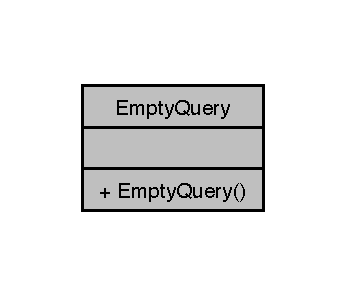
\includegraphics[width=166pt]{class_empty_query__coll__graph}
\end{center}
\end{figure}
\subsection*{Public Member Functions}
\begin{DoxyCompactItemize}
\item 
\hyperlink{class_empty_query_af0f6401966d5bb6d2ff706974bb918b5}{Empty\-Query} (std\-::string query)
\end{DoxyCompactItemize}


\subsection{Detailed Description}
Empty Query class. 

This class defines the Empty Query exception. 

\subsection{Constructor \& Destructor Documentation}
\hypertarget{class_empty_query_af0f6401966d5bb6d2ff706974bb918b5}{\index{Empty\-Query@{Empty\-Query}!Empty\-Query@{Empty\-Query}}
\index{Empty\-Query@{Empty\-Query}!EmptyQuery@{Empty\-Query}}
\subsubsection[{Empty\-Query}]{\setlength{\rightskip}{0pt plus 5cm}Empty\-Query\-::\-Empty\-Query (
\begin{DoxyParamCaption}
\item[{std\-::string}]{query}
\end{DoxyParamCaption}
)\hspace{0.3cm}{\ttfamily [inline]}}}\label{class_empty_query_af0f6401966d5bb6d2ff706974bb918b5}


The documentation for this class was generated from the following file\-:\begin{DoxyCompactItemize}
\item 
\hyperlink{_database_manager_8h}{Database\-Manager.\-h}\end{DoxyCompactItemize}

\hypertarget{class_encomenda}{\section{Encomenda Class Reference}
\label{class_encomenda}\index{Encomenda@{Encomenda}}
}
\subsection*{Public Member Functions}
\begin{DoxyCompactItemize}
\item 
\hypertarget{class_encomenda_acd872b2d444252423746ee7529b48ae8}{{\bfseries Encomenda} (unsigned int id, \hyperlink{class_texto}{Texto} $\ast$texto, std\-::string lingua\-\_\-destino, unsigned int duracao\-\_\-max\-\_\-dias)}\label{class_encomenda_acd872b2d444252423746ee7529b48ae8}

\item 
\hypertarget{class_encomenda_a5009ce207f856836a16e93a6454e93b8}{{\bfseries Encomenda} (unsigned int id, \hyperlink{class_texto}{Texto} $\ast$texto, std\-::string lingua\-\_\-destino, unsigned int duracao\-\_\-max\-\_\-dias, \hyperlink{class_tradutor}{Tradutor} $\ast$tradutor, uint64\-\_\-t timestamp\-\_\-entrega)}\label{class_encomenda_a5009ce207f856836a16e93a6454e93b8}

\item 
\hypertarget{class_encomenda_a600345853bc2238c189de0afcd1c8d09}{unsigned int {\bfseries get\-\_\-id} ()}\label{class_encomenda_a600345853bc2238c189de0afcd1c8d09}

\item 
\hypertarget{class_encomenda_a179dcd8d6ccaa8de0bf87a922c5ce2f8}{unsigned int {\bfseries get\-\_\-duracao\-\_\-max\-\_\-dias} ()}\label{class_encomenda_a179dcd8d6ccaa8de0bf87a922c5ce2f8}

\item 
\hypertarget{class_encomenda_ab3b5fc8fdde834b5c80f42ff0a2bf88b}{void {\bfseries set\-\_\-duracao\-\_\-max\-\_\-dias} (unsigned int dias)}\label{class_encomenda_ab3b5fc8fdde834b5c80f42ff0a2bf88b}

\item 
\hypertarget{class_encomenda_a0a31fd2124968159893d3257b9cadd15}{\hyperlink{class_texto}{Texto} $\ast$ {\bfseries get\-\_\-texto} () const }\label{class_encomenda_a0a31fd2124968159893d3257b9cadd15}

\item 
\hypertarget{class_encomenda_a82f5685295900da96914a1969e3a454f}{void {\bfseries set\-\_\-texto} (\hyperlink{class_texto}{Texto} $\ast$)}\label{class_encomenda_a82f5685295900da96914a1969e3a454f}

\item 
\hypertarget{class_encomenda_a50c1aefd950ca5852e93beec8882db70}{\hyperlink{class_tradutor}{Tradutor} $\ast$ {\bfseries get\-\_\-tradutor} () const }\label{class_encomenda_a50c1aefd950ca5852e93beec8882db70}

\item 
\hypertarget{class_encomenda_af70d8f2344fbae033ed079dfb7350b5a}{void {\bfseries set\-\_\-tradutor} (\hyperlink{class_tradutor}{Tradutor} $\ast$)}\label{class_encomenda_af70d8f2344fbae033ed079dfb7350b5a}

\item 
\hypertarget{class_encomenda_a3b9689429c6ae78580421a96742f9687}{std\-::string {\bfseries get\-\_\-lingua\-\_\-destino} ()}\label{class_encomenda_a3b9689429c6ae78580421a96742f9687}

\item 
\hypertarget{class_encomenda_af8b12f8fba9c65a937f60ed81f9e0770}{void {\bfseries set\-\_\-lingua\-\_\-destino} (std\-::string lingua)}\label{class_encomenda_af8b12f8fba9c65a937f60ed81f9e0770}

\item 
\hypertarget{class_encomenda_a14dd37345213a30a428457f9b5df874d}{uint64\-\_\-t {\bfseries get\-\_\-timestamp\-\_\-entrega} ()}\label{class_encomenda_a14dd37345213a30a428457f9b5df874d}

\item 
\hypertarget{class_encomenda_a894c2ddbe25e0fa49f19fe35134ce3ba}{void {\bfseries set\-\_\-timestamp\-\_\-entrega} (uint64\-\_\-t timestamp\-\_\-entrega)}\label{class_encomenda_a894c2ddbe25e0fa49f19fe35134ce3ba}

\end{DoxyCompactItemize}
\subsection*{Static Public Member Functions}
\begin{DoxyCompactItemize}
\item 
\hypertarget{class_encomenda_a94777b2fe00d586c409b81167e6ee808}{static unsigned int {\bfseries get\-\_\-maior\-\_\-id} ()}\label{class_encomenda_a94777b2fe00d586c409b81167e6ee808}

\end{DoxyCompactItemize}


The documentation for this class was generated from the following files\-:\begin{DoxyCompactItemize}
\item 
Encomenda.\-h\item 
Encomenda.\-cpp\end{DoxyCompactItemize}

\hypertarget{structeqenc}{\section{eqenc Struct Reference}
\label{structeqenc}\index{eqenc@{eqenc}}
}


{\ttfamily \#include $<$Database\-Manager.\-h$>$}



Collaboration diagram for eqenc\-:
\nopagebreak
\begin{figure}[H]
\begin{center}
\leavevmode
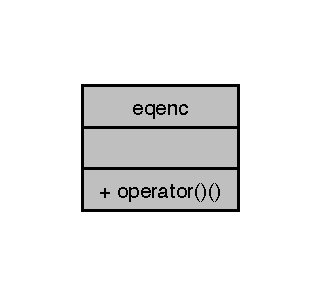
\includegraphics[width=154pt]{structeqenc__coll__graph}
\end{center}
\end{figure}
\subsection*{Public Member Functions}
\begin{DoxyCompactItemize}
\item 
bool \hyperlink{structeqenc_a78ede342f8b12c29786403969e46b426}{operator()} (const \hyperlink{class_encomenda}{Encomenda} \&e1, const \hyperlink{class_encomenda}{Encomenda} \&e2) const 
\end{DoxyCompactItemize}


\subsection{Member Function Documentation}
\hypertarget{structeqenc_a78ede342f8b12c29786403969e46b426}{\index{eqenc@{eqenc}!operator()@{operator()}}
\index{operator()@{operator()}!eqenc@{eqenc}}
\subsubsection[{operator()}]{\setlength{\rightskip}{0pt plus 5cm}bool eqenc\-::operator() (
\begin{DoxyParamCaption}
\item[{const {\bf Encomenda} \&}]{e1, }
\item[{const {\bf Encomenda} \&}]{e2}
\end{DoxyParamCaption}
) const\hspace{0.3cm}{\ttfamily [inline]}}}\label{structeqenc_a78ede342f8b12c29786403969e46b426}


The documentation for this struct was generated from the following file\-:\begin{DoxyCompactItemize}
\item 
\hyperlink{_database_manager_8h}{Database\-Manager.\-h}\end{DoxyCompactItemize}

\hypertarget{structhenc}{\section{henc Struct Reference}
\label{structhenc}\index{henc@{henc}}
}


\hyperlink{class_encomenda}{Encomenda} Hashes.  




{\ttfamily \#include $<$Database\-Manager.\-h$>$}



Collaboration diagram for henc\-:
\nopagebreak
\begin{figure}[H]
\begin{center}
\leavevmode
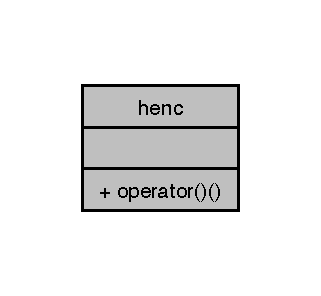
\includegraphics[width=154pt]{structhenc__coll__graph}
\end{center}
\end{figure}
\subsection*{Public Member Functions}
\begin{DoxyCompactItemize}
\item 
int \hyperlink{structhenc_a6facb97d07a25d29092eecaa3ffe4de6}{operator()} (const \hyperlink{class_encomenda}{Encomenda} \&e1) const 
\end{DoxyCompactItemize}


\subsection{Detailed Description}
\hyperlink{class_encomenda}{Encomenda} Hashes. 

This structure defines the hash of an order, for usage with an unordered set. 

\subsection{Member Function Documentation}
\hypertarget{structhenc_a6facb97d07a25d29092eecaa3ffe4de6}{\index{henc@{henc}!operator()@{operator()}}
\index{operator()@{operator()}!henc@{henc}}
\subsubsection[{operator()}]{\setlength{\rightskip}{0pt plus 5cm}int henc\-::operator() (
\begin{DoxyParamCaption}
\item[{const {\bf Encomenda} \&}]{e1}
\end{DoxyParamCaption}
) const\hspace{0.3cm}{\ttfamily [inline]}}}\label{structhenc_a6facb97d07a25d29092eecaa3ffe4de6}


The documentation for this struct was generated from the following file\-:\begin{DoxyCompactItemize}
\item 
\hyperlink{_database_manager_8h}{Database\-Manager.\-h}\end{DoxyCompactItemize}

\hypertarget{class_texto}{\section{Texto Class Reference}
\label{class_texto}\index{Texto@{Texto}}
}


\hyperlink{class_texto}{Texto} /abstract/ class.  




{\ttfamily \#include $<$Texto.\-h$>$}



Inheritance diagram for Texto\-:
\nopagebreak
\begin{figure}[H]
\begin{center}
\leavevmode
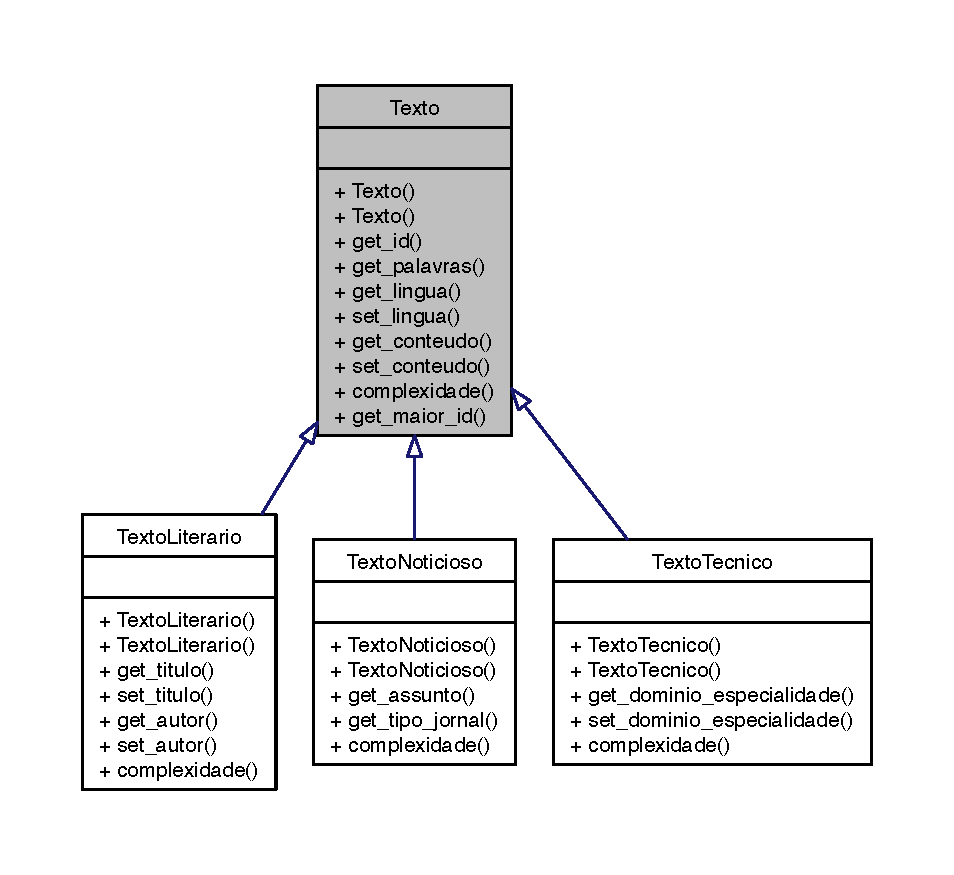
\includegraphics[width=350pt]{class_texto__inherit__graph}
\end{center}
\end{figure}


Collaboration diagram for Texto\-:
\nopagebreak
\begin{figure}[H]
\begin{center}
\leavevmode
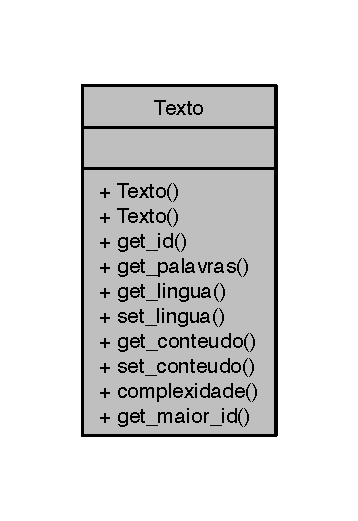
\includegraphics[width=172pt]{class_texto__coll__graph}
\end{center}
\end{figure}
\subsection*{Public Member Functions}
\begin{DoxyCompactItemize}
\item 
\hyperlink{class_texto_a7034548c1e8e2007b0825ef3a01b1b88}{Texto} (unsigned int id, std\-::string lingua, std\-::string conteudo)
\begin{DoxyCompactList}\small\item\em Class Constructor. \end{DoxyCompactList}\item 
\hyperlink{class_texto_a3ccc9eb8eb980eda5e5f6583cbb60425}{Texto} (unsigned int id, std\-::string lingua, unsigned long palavras, std\-::string conteudo)
\begin{DoxyCompactList}\small\item\em Class Constructor. \end{DoxyCompactList}\item 
unsigned int \hyperlink{class_texto_a4e1b7a020c3b1cffe4518937cdd6f565}{get\-\_\-id} ()
\begin{DoxyCompactList}\small\item\em Getter for the I\-D of the text. \end{DoxyCompactList}\item 
unsigned long \hyperlink{class_texto_a35e3a0a47350f735a2e46380eafde1e0}{get\-\_\-palavras} () const 
\begin{DoxyCompactList}\small\item\em Getter for the word count of the text content. \end{DoxyCompactList}\item 
std\-::string \hyperlink{class_texto_adfaca963b37bef9a739def84e2c810b6}{get\-\_\-lingua} ()
\begin{DoxyCompactList}\small\item\em Getter for the language of the text. \end{DoxyCompactList}\item 
void \hyperlink{class_texto_a297021cc2780c0bf398119bf0e4977e0}{set\-\_\-lingua} (std\-::string lingua)
\begin{DoxyCompactList}\small\item\em Setter for the language of the text. \end{DoxyCompactList}\item 
std\-::string \hyperlink{class_texto_a01a9590011195b1a258e2d3bd247ceb0}{get\-\_\-conteudo} ()
\begin{DoxyCompactList}\small\item\em Getter for the text content. \end{DoxyCompactList}\item 
void \hyperlink{class_texto_a94ae33fe47a0ef32a5761a12e097910d}{set\-\_\-conteudo} (std\-::string conteudo)
\begin{DoxyCompactList}\small\item\em Setter for the text content. \end{DoxyCompactList}\item 
virtual unsigned int \hyperlink{class_texto_a92e0fb258179999bc6df2a9da1713a1d}{complexidade} ()=0
\begin{DoxyCompactList}\small\item\em Calculates the complexity of the text. \end{DoxyCompactList}\end{DoxyCompactItemize}
\subsection*{Static Public Member Functions}
\begin{DoxyCompactItemize}
\item 
static unsigned int \hyperlink{class_texto_a674eed23fb437d4f07634f9d6559d325}{get\-\_\-maior\-\_\-id} ()
\begin{DoxyCompactList}\small\item\em Getter for the biggest I\-D of the known text objects. \end{DoxyCompactList}\end{DoxyCompactItemize}


\subsection{Detailed Description}
\hyperlink{class_texto}{Texto} /abstract/ class. 

You should not (alas, can not, most compilers won't even allow it) use this class directly. Please use one of the subclasses (\hyperlink{class_texto_tecnico}{Texto\-Tecnico}, \hyperlink{class_texto_literario}{Texto\-Literario} or \hyperlink{class_texto_noticioso}{Texto\-Noticioso}). 

\subsection{Constructor \& Destructor Documentation}
\hypertarget{class_texto_a7034548c1e8e2007b0825ef3a01b1b88}{\index{Texto@{Texto}!Texto@{Texto}}
\index{Texto@{Texto}!Texto@{Texto}}
\subsubsection[{Texto}]{\setlength{\rightskip}{0pt plus 5cm}Texto\-::\-Texto (
\begin{DoxyParamCaption}
\item[{unsigned int}]{id, }
\item[{std\-::string}]{lingua, }
\item[{std\-::string}]{conteudo}
\end{DoxyParamCaption}
)}}\label{class_texto_a7034548c1e8e2007b0825ef3a01b1b88}


Class Constructor. 


\begin{DoxyParams}{Parameters}
{\em id} & The object I\-D. \\
\hline
{\em lingua} & The language the text is written in. \\
\hline
{\em conteudo} & The plain text contents of the text. \\
\hline
\end{DoxyParams}
\hypertarget{class_texto_a3ccc9eb8eb980eda5e5f6583cbb60425}{\index{Texto@{Texto}!Texto@{Texto}}
\index{Texto@{Texto}!Texto@{Texto}}
\subsubsection[{Texto}]{\setlength{\rightskip}{0pt plus 5cm}Texto\-::\-Texto (
\begin{DoxyParamCaption}
\item[{unsigned int}]{id, }
\item[{std\-::string}]{lingua, }
\item[{unsigned long}]{palavras, }
\item[{std\-::string}]{conteudo}
\end{DoxyParamCaption}
)}}\label{class_texto_a3ccc9eb8eb980eda5e5f6583cbb60425}


Class Constructor. 


\begin{DoxyParams}{Parameters}
{\em id} & The object I\-D. \\
\hline
{\em lingua} & The language the text is written in. \\
\hline
{\em palavras} & The word count of conteudo. \\
\hline
{\em conteudo} & The plain text contents of the text. \\
\hline
\end{DoxyParams}


\subsection{Member Function Documentation}
\hypertarget{class_texto_a92e0fb258179999bc6df2a9da1713a1d}{\index{Texto@{Texto}!complexidade@{complexidade}}
\index{complexidade@{complexidade}!Texto@{Texto}}
\subsubsection[{complexidade}]{\setlength{\rightskip}{0pt plus 5cm}unsigned int Texto\-::complexidade (
\begin{DoxyParamCaption}
{}
\end{DoxyParamCaption}
)\hspace{0.3cm}{\ttfamily [pure virtual]}}}\label{class_texto_a92e0fb258179999bc6df2a9da1713a1d}


Calculates the complexity of the text. 

\begin{DoxyReturn}{Returns}
Complexity value. 
\end{DoxyReturn}


Implemented in \hyperlink{class_texto_literario_a286c1693b71a45d4d577dcd15871892c}{Texto\-Literario}, \hyperlink{class_texto_noticioso_a1db491d92e2a467d258f0f470f994981}{Texto\-Noticioso}, and \hyperlink{class_texto_tecnico_aeeeff7367e226e4fc0f0d4cdb692e85d}{Texto\-Tecnico}.

\hypertarget{class_texto_a01a9590011195b1a258e2d3bd247ceb0}{\index{Texto@{Texto}!get\-\_\-conteudo@{get\-\_\-conteudo}}
\index{get\-\_\-conteudo@{get\-\_\-conteudo}!Texto@{Texto}}
\subsubsection[{get\-\_\-conteudo}]{\setlength{\rightskip}{0pt plus 5cm}std\-::string Texto\-::get\-\_\-conteudo (
\begin{DoxyParamCaption}
{}
\end{DoxyParamCaption}
)}}\label{class_texto_a01a9590011195b1a258e2d3bd247ceb0}


Getter for the text content. 

\begin{DoxyReturn}{Returns}
Text Content (in plain text). 
\end{DoxyReturn}
\hypertarget{class_texto_a4e1b7a020c3b1cffe4518937cdd6f565}{\index{Texto@{Texto}!get\-\_\-id@{get\-\_\-id}}
\index{get\-\_\-id@{get\-\_\-id}!Texto@{Texto}}
\subsubsection[{get\-\_\-id}]{\setlength{\rightskip}{0pt plus 5cm}unsigned int Texto\-::get\-\_\-id (
\begin{DoxyParamCaption}
{}
\end{DoxyParamCaption}
)}}\label{class_texto_a4e1b7a020c3b1cffe4518937cdd6f565}


Getter for the I\-D of the text. 

\begin{DoxyReturn}{Returns}
The I\-D. 
\end{DoxyReturn}
\hypertarget{class_texto_adfaca963b37bef9a739def84e2c810b6}{\index{Texto@{Texto}!get\-\_\-lingua@{get\-\_\-lingua}}
\index{get\-\_\-lingua@{get\-\_\-lingua}!Texto@{Texto}}
\subsubsection[{get\-\_\-lingua}]{\setlength{\rightskip}{0pt plus 5cm}std\-::string Texto\-::get\-\_\-lingua (
\begin{DoxyParamCaption}
{}
\end{DoxyParamCaption}
)}}\label{class_texto_adfaca963b37bef9a739def84e2c810b6}


Getter for the language of the text. 

\begin{DoxyReturn}{Returns}
Language of the text. 
\end{DoxyReturn}
\hypertarget{class_texto_a674eed23fb437d4f07634f9d6559d325}{\index{Texto@{Texto}!get\-\_\-maior\-\_\-id@{get\-\_\-maior\-\_\-id}}
\index{get\-\_\-maior\-\_\-id@{get\-\_\-maior\-\_\-id}!Texto@{Texto}}
\subsubsection[{get\-\_\-maior\-\_\-id}]{\setlength{\rightskip}{0pt plus 5cm}unsigned int Texto\-::get\-\_\-maior\-\_\-id (
\begin{DoxyParamCaption}
{}
\end{DoxyParamCaption}
)\hspace{0.3cm}{\ttfamily [static]}}}\label{class_texto_a674eed23fb437d4f07634f9d6559d325}


Getter for the biggest I\-D of the known text objects. 

\begin{DoxyReturn}{Returns}
The biggest known I\-D. 
\end{DoxyReturn}
\hypertarget{class_texto_a35e3a0a47350f735a2e46380eafde1e0}{\index{Texto@{Texto}!get\-\_\-palavras@{get\-\_\-palavras}}
\index{get\-\_\-palavras@{get\-\_\-palavras}!Texto@{Texto}}
\subsubsection[{get\-\_\-palavras}]{\setlength{\rightskip}{0pt plus 5cm}unsigned long Texto\-::get\-\_\-palavras (
\begin{DoxyParamCaption}
{}
\end{DoxyParamCaption}
) const}}\label{class_texto_a35e3a0a47350f735a2e46380eafde1e0}


Getter for the word count of the text content. 

\begin{DoxyReturn}{Returns}
Word Count of the text content. 
\end{DoxyReturn}
\hypertarget{class_texto_a94ae33fe47a0ef32a5761a12e097910d}{\index{Texto@{Texto}!set\-\_\-conteudo@{set\-\_\-conteudo}}
\index{set\-\_\-conteudo@{set\-\_\-conteudo}!Texto@{Texto}}
\subsubsection[{set\-\_\-conteudo}]{\setlength{\rightskip}{0pt plus 5cm}void Texto\-::set\-\_\-conteudo (
\begin{DoxyParamCaption}
\item[{std\-::string}]{conteudo}
\end{DoxyParamCaption}
)}}\label{class_texto_a94ae33fe47a0ef32a5761a12e097910d}


Setter for the text content. 

\begin{DoxyReturn}{Returns}
Text Content (in plain text). 
\end{DoxyReturn}
\hypertarget{class_texto_a297021cc2780c0bf398119bf0e4977e0}{\index{Texto@{Texto}!set\-\_\-lingua@{set\-\_\-lingua}}
\index{set\-\_\-lingua@{set\-\_\-lingua}!Texto@{Texto}}
\subsubsection[{set\-\_\-lingua}]{\setlength{\rightskip}{0pt plus 5cm}void Texto\-::set\-\_\-lingua (
\begin{DoxyParamCaption}
\item[{std\-::string}]{lingua}
\end{DoxyParamCaption}
)}}\label{class_texto_a297021cc2780c0bf398119bf0e4977e0}


Setter for the language of the text. 


\begin{DoxyParams}{Parameters}
{\em lingua} & Language of the text. \\
\hline
\end{DoxyParams}


The documentation for this class was generated from the following files\-:\begin{DoxyCompactItemize}
\item 
\hyperlink{_texto_8h}{Texto.\-h}\item 
\hyperlink{_texto_8cpp}{Texto.\-cpp}\end{DoxyCompactItemize}

\hypertarget{class_texto_literario}{\section{Texto\-Literario Class Reference}
\label{class_texto_literario}\index{Texto\-Literario@{Texto\-Literario}}
}


\hyperlink{class_texto}{Texto} Literario class.  




{\ttfamily \#include $<$Texto\-Literario.\-h$>$}



Inheritance diagram for Texto\-Literario\-:
\nopagebreak
\begin{figure}[H]
\begin{center}
\leavevmode
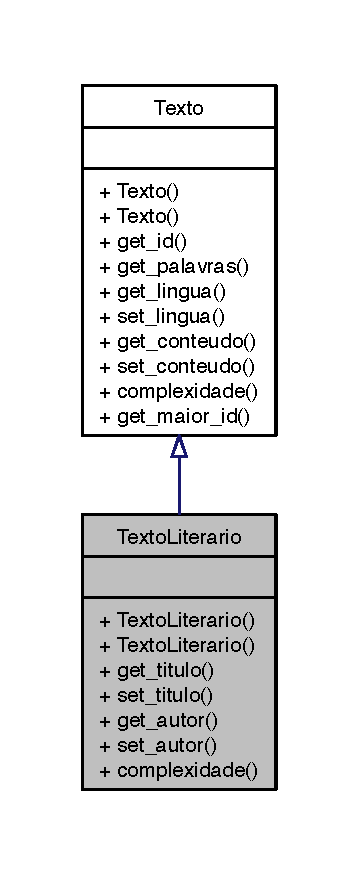
\includegraphics[width=172pt]{class_texto_literario__inherit__graph}
\end{center}
\end{figure}


Collaboration diagram for Texto\-Literario\-:
\nopagebreak
\begin{figure}[H]
\begin{center}
\leavevmode
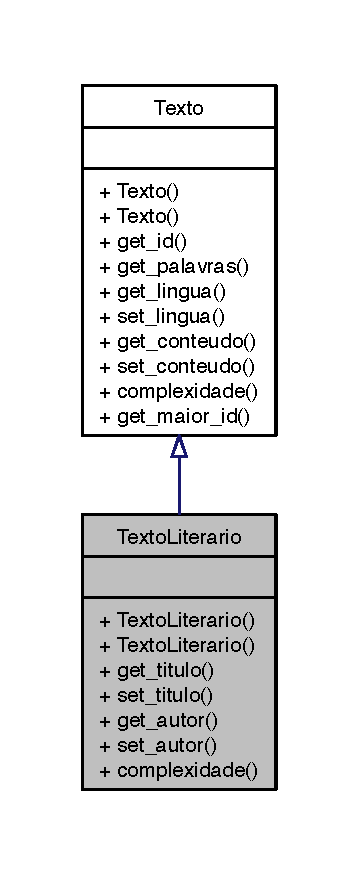
\includegraphics[width=172pt]{class_texto_literario__coll__graph}
\end{center}
\end{figure}
\subsection*{Public Member Functions}
\begin{DoxyCompactItemize}
\item 
\hyperlink{class_texto_literario_addeb2b30770693455c5395a4a3fb941c}{Texto\-Literario} (unsigned int id, std\-::string lingua, std\-::string conteudo, std\-::string titulo, std\-::string autor)
\begin{DoxyCompactList}\small\item\em Class Constructor. \end{DoxyCompactList}\item 
\hyperlink{class_texto_literario_ac8484056631c263a653243b80065114b}{Texto\-Literario} (unsigned int id, std\-::string lingua, unsigned long palavras, std\-::string conteudo, std\-::string titulo, std\-::string autor)
\begin{DoxyCompactList}\small\item\em Class Constructor. \end{DoxyCompactList}\item 
std\-::string \hyperlink{class_texto_literario_adca504c785afdb9e77542b2bdca90a37}{get\-\_\-titulo} ()
\begin{DoxyCompactList}\small\item\em Getter for the title of the text. \end{DoxyCompactList}\item 
void \hyperlink{class_texto_literario_acfb7945b3d45250c316a3b6dc688383c}{set\-\_\-titulo} (std\-::string titulo)
\begin{DoxyCompactList}\small\item\em Setter for the title of the text. \end{DoxyCompactList}\item 
std\-::string \hyperlink{class_texto_literario_acb31c6be6750cea439dde8636bf960ff}{get\-\_\-autor} ()
\begin{DoxyCompactList}\small\item\em Getter for the author of the text. \end{DoxyCompactList}\item 
void \hyperlink{class_texto_literario_a859bcc3c015ebcced7b4691990d3ec2a}{set\-\_\-autor} (std\-::string autor)
\begin{DoxyCompactList}\small\item\em Setter for the author of the text. \end{DoxyCompactList}\item 
unsigned int \hyperlink{class_texto_literario_a286c1693b71a45d4d577dcd15871892c}{complexidade} ()
\begin{DoxyCompactList}\small\item\em Calculates the complexity of the text. \end{DoxyCompactList}\end{DoxyCompactItemize}
\subsection*{Additional Inherited Members}


\subsection{Detailed Description}
\hyperlink{class_texto}{Texto} Literario class. 

Subclass of \hyperlink{class_texto}{Texto}, this handles a specific type of Text (Literary Text). 

\subsection{Constructor \& Destructor Documentation}
\hypertarget{class_texto_literario_addeb2b30770693455c5395a4a3fb941c}{\index{Texto\-Literario@{Texto\-Literario}!Texto\-Literario@{Texto\-Literario}}
\index{Texto\-Literario@{Texto\-Literario}!TextoLiterario@{Texto\-Literario}}
\subsubsection[{Texto\-Literario}]{\setlength{\rightskip}{0pt plus 5cm}Texto\-Literario\-::\-Texto\-Literario (
\begin{DoxyParamCaption}
\item[{unsigned int}]{id, }
\item[{std\-::string}]{lingua, }
\item[{std\-::string}]{conteudo, }
\item[{std\-::string}]{titulo, }
\item[{std\-::string}]{autor}
\end{DoxyParamCaption}
)}}\label{class_texto_literario_addeb2b30770693455c5395a4a3fb941c}


Class Constructor. 


\begin{DoxyParams}{Parameters}
{\em id} & The object I\-D. \\
\hline
{\em lingua} & The language the text is written in. \\
\hline
{\em conteudo} & The plain text contents of the text. \\
\hline
{\em titulo} & The title of the text. \\
\hline
{\em autor} & The author of the text. \\
\hline
\end{DoxyParams}
\hypertarget{class_texto_literario_ac8484056631c263a653243b80065114b}{\index{Texto\-Literario@{Texto\-Literario}!Texto\-Literario@{Texto\-Literario}}
\index{Texto\-Literario@{Texto\-Literario}!TextoLiterario@{Texto\-Literario}}
\subsubsection[{Texto\-Literario}]{\setlength{\rightskip}{0pt plus 5cm}Texto\-Literario\-::\-Texto\-Literario (
\begin{DoxyParamCaption}
\item[{unsigned int}]{id, }
\item[{std\-::string}]{lingua, }
\item[{unsigned long}]{palavras, }
\item[{std\-::string}]{conteudo, }
\item[{std\-::string}]{titulo, }
\item[{std\-::string}]{autor}
\end{DoxyParamCaption}
)}}\label{class_texto_literario_ac8484056631c263a653243b80065114b}


Class Constructor. 


\begin{DoxyParams}{Parameters}
{\em id} & The object I\-D. \\
\hline
{\em lingua} & The language the text is written in. \\
\hline
{\em palavras} & The word coint of conteudo. \\
\hline
{\em conteudo} & The plain text contents of the text. \\
\hline
{\em titulo} & The title of the text. \\
\hline
{\em autor} & The author of the text. \\
\hline
\end{DoxyParams}


\subsection{Member Function Documentation}
\hypertarget{class_texto_literario_a286c1693b71a45d4d577dcd15871892c}{\index{Texto\-Literario@{Texto\-Literario}!complexidade@{complexidade}}
\index{complexidade@{complexidade}!TextoLiterario@{Texto\-Literario}}
\subsubsection[{complexidade}]{\setlength{\rightskip}{0pt plus 5cm}unsigned int Texto\-Literario\-::complexidade (
\begin{DoxyParamCaption}
{}
\end{DoxyParamCaption}
)\hspace{0.3cm}{\ttfamily [virtual]}}}\label{class_texto_literario_a286c1693b71a45d4d577dcd15871892c}


Calculates the complexity of the text. 

\begin{DoxyReturn}{Returns}
Complexity value. 
\end{DoxyReturn}


Reimplemented from \hyperlink{class_texto_a9b397139df00ed907e1e6a1c29e2429b}{Texto}.

\hypertarget{class_texto_literario_acb31c6be6750cea439dde8636bf960ff}{\index{Texto\-Literario@{Texto\-Literario}!get\-\_\-autor@{get\-\_\-autor}}
\index{get\-\_\-autor@{get\-\_\-autor}!TextoLiterario@{Texto\-Literario}}
\subsubsection[{get\-\_\-autor}]{\setlength{\rightskip}{0pt plus 5cm}std\-::string Texto\-Literario\-::get\-\_\-autor (
\begin{DoxyParamCaption}
{}
\end{DoxyParamCaption}
)}}\label{class_texto_literario_acb31c6be6750cea439dde8636bf960ff}


Getter for the author of the text. 

\begin{DoxyReturn}{Returns}
The author of the text. 
\end{DoxyReturn}
\hypertarget{class_texto_literario_adca504c785afdb9e77542b2bdca90a37}{\index{Texto\-Literario@{Texto\-Literario}!get\-\_\-titulo@{get\-\_\-titulo}}
\index{get\-\_\-titulo@{get\-\_\-titulo}!TextoLiterario@{Texto\-Literario}}
\subsubsection[{get\-\_\-titulo}]{\setlength{\rightskip}{0pt plus 5cm}std\-::string Texto\-Literario\-::get\-\_\-titulo (
\begin{DoxyParamCaption}
{}
\end{DoxyParamCaption}
)}}\label{class_texto_literario_adca504c785afdb9e77542b2bdca90a37}


Getter for the title of the text. 

\begin{DoxyReturn}{Returns}
The title of the text. 
\end{DoxyReturn}
\hypertarget{class_texto_literario_a859bcc3c015ebcced7b4691990d3ec2a}{\index{Texto\-Literario@{Texto\-Literario}!set\-\_\-autor@{set\-\_\-autor}}
\index{set\-\_\-autor@{set\-\_\-autor}!TextoLiterario@{Texto\-Literario}}
\subsubsection[{set\-\_\-autor}]{\setlength{\rightskip}{0pt plus 5cm}void Texto\-Literario\-::set\-\_\-autor (
\begin{DoxyParamCaption}
\item[{std\-::string}]{autor}
\end{DoxyParamCaption}
)}}\label{class_texto_literario_a859bcc3c015ebcced7b4691990d3ec2a}


Setter for the author of the text. 

\begin{DoxyReturn}{Returns}
The author of the text. 
\end{DoxyReturn}
\hypertarget{class_texto_literario_acfb7945b3d45250c316a3b6dc688383c}{\index{Texto\-Literario@{Texto\-Literario}!set\-\_\-titulo@{set\-\_\-titulo}}
\index{set\-\_\-titulo@{set\-\_\-titulo}!TextoLiterario@{Texto\-Literario}}
\subsubsection[{set\-\_\-titulo}]{\setlength{\rightskip}{0pt plus 5cm}void Texto\-Literario\-::set\-\_\-titulo (
\begin{DoxyParamCaption}
\item[{std\-::string}]{titulo}
\end{DoxyParamCaption}
)}}\label{class_texto_literario_acfb7945b3d45250c316a3b6dc688383c}


Setter for the title of the text. 

\begin{DoxyReturn}{Returns}
The title of the text. 
\end{DoxyReturn}


The documentation for this class was generated from the following files\-:\begin{DoxyCompactItemize}
\item 
\hyperlink{_texto_literario_8h}{Texto\-Literario.\-h}\item 
\hyperlink{_texto_literario_8cpp}{Texto\-Literario.\-cpp}\end{DoxyCompactItemize}

\hypertarget{class_texto_noticioso}{\section{Texto\-Noticioso Class Reference}
\label{class_texto_noticioso}\index{Texto\-Noticioso@{Texto\-Noticioso}}
}
Inheritance diagram for Texto\-Noticioso\-:\begin{figure}[H]
\begin{center}
\leavevmode
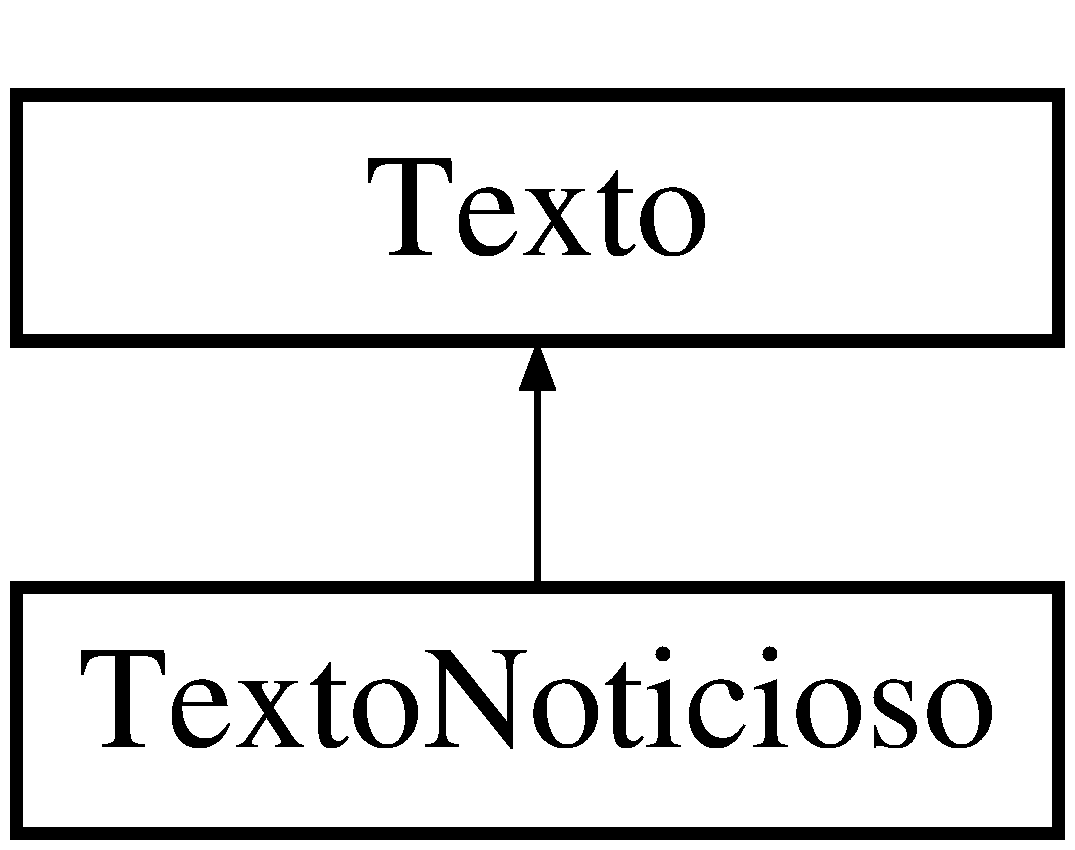
\includegraphics[height=2.000000cm]{class_texto_noticioso}
\end{center}
\end{figure}
\subsection*{Public Member Functions}
\begin{DoxyCompactItemize}
\item 
\hypertarget{class_texto_noticioso_a74a984b14609c5ad38a32cefcc5c9da7}{{\bfseries Texto\-Noticioso} (unsigned int id, std\-::string lingua, std\-::string conteudo, std\-::string assunto, tipo\-\_\-jornal tipo)}\label{class_texto_noticioso_a74a984b14609c5ad38a32cefcc5c9da7}

\item 
\hypertarget{class_texto_noticioso_a9b82b7cd28537c9aa6c214d3439ab6f5}{{\bfseries Texto\-Noticioso} (unsigned int id, std\-::string lingua, unsigned long palavras, std\-::string conteudo, std\-::string assunto, tipo\-\_\-jornal tipo)}\label{class_texto_noticioso_a9b82b7cd28537c9aa6c214d3439ab6f5}

\item 
\hypertarget{class_texto_noticioso_afd686397a10b9e6afa8eb9f1aaf5d21e}{std\-::string {\bfseries get\-\_\-assunto} ()}\label{class_texto_noticioso_afd686397a10b9e6afa8eb9f1aaf5d21e}

\item 
\hypertarget{class_texto_noticioso_ac0edd9121ef61cb4adc360faabecd62b}{tipo\-\_\-jornal {\bfseries get\-\_\-tipo\-\_\-jornal} ()}\label{class_texto_noticioso_ac0edd9121ef61cb4adc360faabecd62b}

\item 
\hypertarget{class_texto_noticioso_a5179276c932815f134aa1e70a6840d64}{unsigned int {\bfseries get\-\_\-complexidade} ()}\label{class_texto_noticioso_a5179276c932815f134aa1e70a6840d64}

\end{DoxyCompactItemize}
\subsection*{Additional Inherited Members}


The documentation for this class was generated from the following files\-:\begin{DoxyCompactItemize}
\item 
Texto\-Noticioso.\-h\item 
Texto\-Noticioso.\-cpp\end{DoxyCompactItemize}

\hypertarget{class_texto_tecnico}{\section{Texto\-Tecnico Class Reference}
\label{class_texto_tecnico}\index{Texto\-Tecnico@{Texto\-Tecnico}}
}


\hyperlink{class_texto}{Texto} Tecnico class.  




{\ttfamily \#include $<$Texto\-Tecnico.\-h$>$}



Inheritance diagram for Texto\-Tecnico\-:
\nopagebreak
\begin{figure}[H]
\begin{center}
\leavevmode
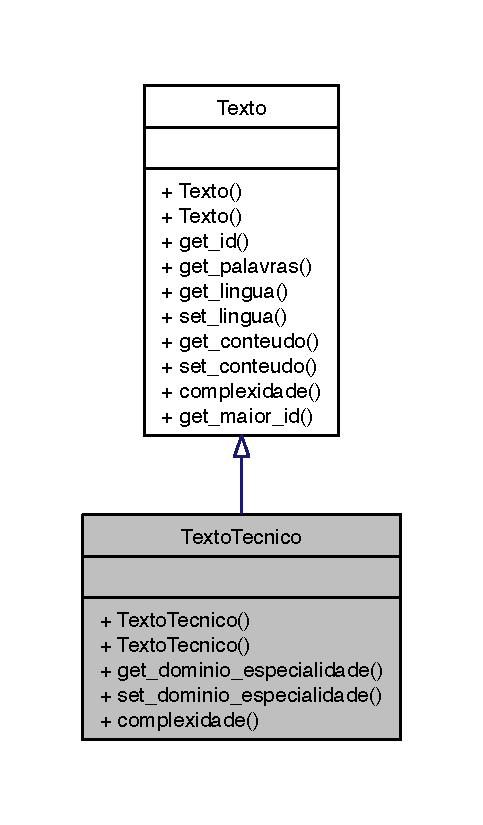
\includegraphics[width=232pt]{class_texto_tecnico__inherit__graph}
\end{center}
\end{figure}
\subsection*{Public Member Functions}
\begin{DoxyCompactItemize}
\item 
\hyperlink{class_texto_tecnico_a4c770469d3a65f750b4551bef18629a9}{Texto\-Tecnico} (unsigned int id, std\-::string lingua, std\-::string conteudo, std\-::string dominio\-\_\-especialidade)
\begin{DoxyCompactList}\small\item\em Class Constructor. \end{DoxyCompactList}\item 
\hyperlink{class_texto_tecnico_adc11a5c4366f90c1f22fc986c4bc2131}{Texto\-Tecnico} (unsigned int id, std\-::string lingua, unsigned long palavras, std\-::string conteudo, std\-::string dominio\-\_\-especialidade)
\begin{DoxyCompactList}\small\item\em Class Constructor. \end{DoxyCompactList}\item 
std\-::string \hyperlink{class_texto_tecnico_af0541bfc3a8fc861eb13abba28a6768d}{get\-\_\-dominio\-\_\-especialidade} ()
\begin{DoxyCompactList}\small\item\em Getter for the text domain. \end{DoxyCompactList}\item 
void \hyperlink{class_texto_tecnico_af66d0b574c0e3316870fb8fdc3223c74}{set\-\_\-dominio\-\_\-especialidade} (std\-::string dominio)
\begin{DoxyCompactList}\small\item\em Setter for the text domain. \end{DoxyCompactList}\item 
unsigned int \hyperlink{class_texto_tecnico_aeeeff7367e226e4fc0f0d4cdb692e85d}{complexidade} ()
\begin{DoxyCompactList}\small\item\em Calculates the complexity of the text. \end{DoxyCompactList}\end{DoxyCompactItemize}
\subsection*{Additional Inherited Members}


\subsection{Detailed Description}
\hyperlink{class_texto}{Texto} Tecnico class. 

Subclass of \hyperlink{class_texto}{Texto}, this handles a specific type of Text (Technical Text). 

\subsection{Constructor \& Destructor Documentation}
\hypertarget{class_texto_tecnico_a4c770469d3a65f750b4551bef18629a9}{\index{Texto\-Tecnico@{Texto\-Tecnico}!Texto\-Tecnico@{Texto\-Tecnico}}
\index{Texto\-Tecnico@{Texto\-Tecnico}!TextoTecnico@{Texto\-Tecnico}}
\subsubsection[{Texto\-Tecnico}]{\setlength{\rightskip}{0pt plus 5cm}Texto\-Tecnico\-::\-Texto\-Tecnico (
\begin{DoxyParamCaption}
\item[{unsigned int}]{id, }
\item[{std\-::string}]{lingua, }
\item[{std\-::string}]{conteudo, }
\item[{std\-::string}]{dominio\-\_\-especialidade}
\end{DoxyParamCaption}
)}}\label{class_texto_tecnico_a4c770469d3a65f750b4551bef18629a9}


Class Constructor. 


\begin{DoxyParams}{Parameters}
{\em id} & The object I\-D. \\
\hline
{\em lingua} & The language the text is written in. \\
\hline
{\em conteudo} & The plain text contents of the text. \\
\hline
{\em dominio\-\_\-especialidade} & The domain of the contents of the text. \\
\hline
\end{DoxyParams}
\hypertarget{class_texto_tecnico_adc11a5c4366f90c1f22fc986c4bc2131}{\index{Texto\-Tecnico@{Texto\-Tecnico}!Texto\-Tecnico@{Texto\-Tecnico}}
\index{Texto\-Tecnico@{Texto\-Tecnico}!TextoTecnico@{Texto\-Tecnico}}
\subsubsection[{Texto\-Tecnico}]{\setlength{\rightskip}{0pt plus 5cm}Texto\-Tecnico\-::\-Texto\-Tecnico (
\begin{DoxyParamCaption}
\item[{unsigned int}]{id, }
\item[{std\-::string}]{lingua, }
\item[{unsigned long}]{palavras, }
\item[{std\-::string}]{conteudo, }
\item[{std\-::string}]{dominio\-\_\-especialidade}
\end{DoxyParamCaption}
)}}\label{class_texto_tecnico_adc11a5c4366f90c1f22fc986c4bc2131}


Class Constructor. 


\begin{DoxyParams}{Parameters}
{\em id} & The object I\-D. \\
\hline
{\em lingua} & The language the text is written in. \\
\hline
{\em palavras} & The word coint of conteudo. \\
\hline
{\em conteudo} & The plain text contents of the text. \\
\hline
{\em dominio\-\_\-especialidade} & The domain of the contents of the text. \\
\hline
\end{DoxyParams}


\subsection{Member Function Documentation}
\hypertarget{class_texto_tecnico_aeeeff7367e226e4fc0f0d4cdb692e85d}{\index{Texto\-Tecnico@{Texto\-Tecnico}!complexidade@{complexidade}}
\index{complexidade@{complexidade}!TextoTecnico@{Texto\-Tecnico}}
\subsubsection[{complexidade}]{\setlength{\rightskip}{0pt plus 5cm}unsigned int Texto\-Tecnico\-::complexidade (
\begin{DoxyParamCaption}
{}
\end{DoxyParamCaption}
)\hspace{0.3cm}{\ttfamily [virtual]}}}\label{class_texto_tecnico_aeeeff7367e226e4fc0f0d4cdb692e85d}


Calculates the complexity of the text. 

\begin{DoxyReturn}{Returns}
Complexity value. 
\end{DoxyReturn}


Reimplemented from \hyperlink{class_texto_a9b397139df00ed907e1e6a1c29e2429b}{Texto}.

\hypertarget{class_texto_tecnico_af0541bfc3a8fc861eb13abba28a6768d}{\index{Texto\-Tecnico@{Texto\-Tecnico}!get\-\_\-dominio\-\_\-especialidade@{get\-\_\-dominio\-\_\-especialidade}}
\index{get\-\_\-dominio\-\_\-especialidade@{get\-\_\-dominio\-\_\-especialidade}!TextoTecnico@{Texto\-Tecnico}}
\subsubsection[{get\-\_\-dominio\-\_\-especialidade}]{\setlength{\rightskip}{0pt plus 5cm}std\-::string Texto\-Tecnico\-::get\-\_\-dominio\-\_\-especialidade (
\begin{DoxyParamCaption}
{}
\end{DoxyParamCaption}
)}}\label{class_texto_tecnico_af0541bfc3a8fc861eb13abba28a6768d}


Getter for the text domain. 

\begin{DoxyReturn}{Returns}
The domain of the text. 
\end{DoxyReturn}
\hypertarget{class_texto_tecnico_af66d0b574c0e3316870fb8fdc3223c74}{\index{Texto\-Tecnico@{Texto\-Tecnico}!set\-\_\-dominio\-\_\-especialidade@{set\-\_\-dominio\-\_\-especialidade}}
\index{set\-\_\-dominio\-\_\-especialidade@{set\-\_\-dominio\-\_\-especialidade}!TextoTecnico@{Texto\-Tecnico}}
\subsubsection[{set\-\_\-dominio\-\_\-especialidade}]{\setlength{\rightskip}{0pt plus 5cm}void Texto\-Tecnico\-::set\-\_\-dominio\-\_\-especialidade (
\begin{DoxyParamCaption}
\item[{std\-::string}]{dominio}
\end{DoxyParamCaption}
)}}\label{class_texto_tecnico_af66d0b574c0e3316870fb8fdc3223c74}


Setter for the text domain. 


\begin{DoxyParams}{Parameters}
{\em dominio} & The domain of the text. \\
\hline
\end{DoxyParams}


The documentation for this class was generated from the following files\-:\begin{DoxyCompactItemize}
\item 
\hyperlink{_texto_tecnico_8h}{Texto\-Tecnico.\-h}\item 
\hyperlink{_texto_tecnico_8cpp}{Texto\-Tecnico.\-cpp}\end{DoxyCompactItemize}

\hypertarget{class_tradutor}{\section{Tradutor Class Reference}
\label{class_tradutor}\index{Tradutor@{Tradutor}}
}


\hyperlink{class_tradutor}{Tradutor} class.  




{\ttfamily \#include $<$Tradutor.\-h$>$}



Collaboration diagram for Tradutor\-:
\nopagebreak
\begin{figure}[H]
\begin{center}
\leavevmode
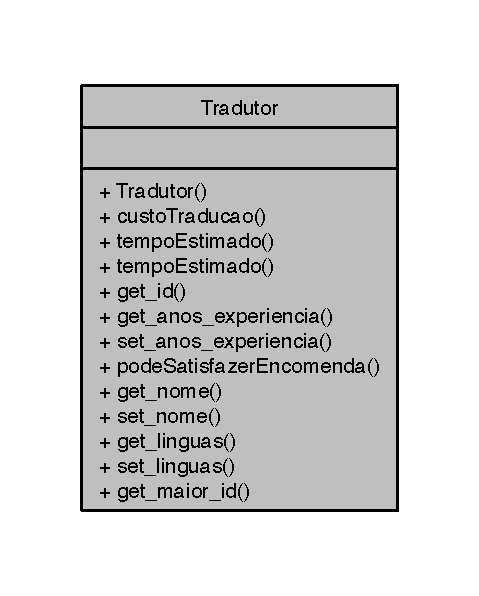
\includegraphics[width=230pt]{class_tradutor__coll__graph}
\end{center}
\end{figure}
\subsection*{Public Member Functions}
\begin{DoxyCompactItemize}
\item 
\hyperlink{class_tradutor_a856f362e6c97ea42d04875e6c9d012e3}{Tradutor} (unsigned int id, std\-::string nome, unsigned int anos\-\_\-experiencia, std\-::vector$<$ std\-::string $>$ linguas)
\begin{DoxyCompactList}\small\item\em Class Constructor. \end{DoxyCompactList}\item 
\hyperlink{class_tradutor_a8b918326e5d4ad49250a87dcab4de424}{Tradutor} (unsigned int id, std\-::string nome, unsigned int anos\-\_\-experiencia, std\-::vector$<$ std\-::string $>$ linguas, bool contratado)
\begin{DoxyCompactList}\small\item\em Class Constructor. \end{DoxyCompactList}\item 
double \hyperlink{class_tradutor_ab55718903fb3e7cc5c1b21b87d64393a}{custo\-Traducao} (\hyperlink{class_texto}{Texto} $\ast$texto)
\begin{DoxyCompactList}\small\item\em Calculates the cost of a given translation. \end{DoxyCompactList}\item 
unsigned int \hyperlink{class_tradutor_a1ca7c608db7e9145e8b9105e19e5900a}{tempo\-Estimado} (\hyperlink{class_texto}{Texto} $\ast$text)
\begin{DoxyCompactList}\small\item\em Calculates the time to fullfill a translation. \end{DoxyCompactList}\item 
unsigned int \hyperlink{class_tradutor_acd53cf00b851be61350100c9aa6ef3c0}{tempo\-Estimado} (\hyperlink{class_encomenda}{Encomenda} $\ast$encomenda)
\begin{DoxyCompactList}\small\item\em Calculates the time to fullfill a given order. \end{DoxyCompactList}\item 
unsigned int \hyperlink{class_tradutor_adc3d4f5ae46ebd92072c644f9fe0e479}{get\-\_\-id} ()
\begin{DoxyCompactList}\small\item\em Getter for the I\-D of the translator. \end{DoxyCompactList}\item 
unsigned int \hyperlink{class_tradutor_a001f11f69661085cb11192d3c6f5d556}{get\-\_\-anos\-\_\-experiencia} ()
\begin{DoxyCompactList}\small\item\em Getter for the years of experience of the translator. \end{DoxyCompactList}\item 
void \hyperlink{class_tradutor_a938cfc1c263b3504fc4d7fbdc939b087}{set\-\_\-anos\-\_\-experiencia} (unsigned int anos\-\_\-exp)
\begin{DoxyCompactList}\small\item\em Setter for the years of experience of the translator. \end{DoxyCompactList}\item 
bool \hyperlink{class_tradutor_a1d22a38c8eaa3753d44b521bb3aab2af}{pode\-Satisfazer\-Encomenda} (\hyperlink{class_encomenda}{Encomenda} $\ast$encomenda)
\begin{DoxyCompactList}\small\item\em Checks if the translator is able to fullfill a given translation. \end{DoxyCompactList}\item 
std\-::string \hyperlink{class_tradutor_aada5c883969bb7903924f2f2ae376026}{get\-\_\-nome} () const 
\begin{DoxyCompactList}\small\item\em Getter for name of the translator. \end{DoxyCompactList}\item 
void \hyperlink{class_tradutor_aa50fdceab0ca03dfe5c2a1639bc5869e}{set\-\_\-nome} (std\-::string nome)
\begin{DoxyCompactList}\small\item\em Setter for name of the translator. \end{DoxyCompactList}\item 
std\-::vector$<$ std\-::string $>$ \hyperlink{class_tradutor_a011b86fa2dae11c6ccdda1cbeb844e94}{get\-\_\-linguas} ()
\begin{DoxyCompactList}\small\item\em Getter for the languages known to the translator. \end{DoxyCompactList}\item 
void \hyperlink{class_tradutor_a83ed5b48e00f3a15c579e209bb01d53f}{set\-\_\-linguas} (std\-::vector$<$ std\-::string $>$ linguas)
\begin{DoxyCompactList}\small\item\em Setter for the languages known to the translator. \end{DoxyCompactList}\item 
bool \hyperlink{class_tradutor_abfd51adb78973d8bbc3bbd35eb5d5b94}{get\-\_\-contratado} ()
\begin{DoxyCompactList}\small\item\em Getter for employment status of the translator. \end{DoxyCompactList}\item 
void \hyperlink{class_tradutor_a00b1ffa1dc1a0eb9fabf6e240a61b94b}{set\-\_\-contratado} (bool cont)
\begin{DoxyCompactList}\small\item\em Setter for employment status of the translator. \end{DoxyCompactList}\item 
bool \hyperlink{class_tradutor_a33f43a54dbef52d8a25796c5ecd6c00a}{operator$<$} (const \hyperlink{class_tradutor}{Tradutor} \&trad) const 
\begin{DoxyCompactList}\small\item\em Overloaded comparision $<$ operator. \end{DoxyCompactList}\end{DoxyCompactItemize}
\subsection*{Static Public Member Functions}
\begin{DoxyCompactItemize}
\item 
static unsigned int \hyperlink{class_tradutor_af2caad7e33c443f238851c5bb2d63930}{get\-\_\-maior\-\_\-id} ()
\begin{DoxyCompactList}\small\item\em Getter for the biggest translator I\-D (of all known translators). \end{DoxyCompactList}\end{DoxyCompactItemize}


\subsection{Detailed Description}
\hyperlink{class_tradutor}{Tradutor} class. 

This class packages the details about a translator and provides some functionality on them. 

\subsection{Constructor \& Destructor Documentation}
\hypertarget{class_tradutor_a856f362e6c97ea42d04875e6c9d012e3}{\index{Tradutor@{Tradutor}!Tradutor@{Tradutor}}
\index{Tradutor@{Tradutor}!Tradutor@{Tradutor}}
\subsubsection[{Tradutor}]{\setlength{\rightskip}{0pt plus 5cm}Tradutor\-::\-Tradutor (
\begin{DoxyParamCaption}
\item[{unsigned int}]{id, }
\item[{std\-::string}]{nome, }
\item[{unsigned int}]{anos\-\_\-experiencia, }
\item[{std\-::vector$<$ std\-::string $>$}]{linguas}
\end{DoxyParamCaption}
)}}\label{class_tradutor_a856f362e6c97ea42d04875e6c9d012e3}


Class Constructor. 


\begin{DoxyParams}{Parameters}
{\em id} & The object I\-D. \\
\hline
{\em nome} & The name of the translator. \\
\hline
{\em anos\-\_\-experiencia} & The experience of the translator, in years. Should be at least 1. \\
\hline
{\em linguas} & The maximum number of days the order should be fullfilled in. \\
\hline
\end{DoxyParams}
\hypertarget{class_tradutor_a8b918326e5d4ad49250a87dcab4de424}{\index{Tradutor@{Tradutor}!Tradutor@{Tradutor}}
\index{Tradutor@{Tradutor}!Tradutor@{Tradutor}}
\subsubsection[{Tradutor}]{\setlength{\rightskip}{0pt plus 5cm}Tradutor\-::\-Tradutor (
\begin{DoxyParamCaption}
\item[{unsigned int}]{id, }
\item[{std\-::string}]{nome, }
\item[{unsigned int}]{anos\-\_\-experiencia, }
\item[{std\-::vector$<$ std\-::string $>$}]{linguas, }
\item[{bool}]{contratado}
\end{DoxyParamCaption}
)}}\label{class_tradutor_a8b918326e5d4ad49250a87dcab4de424}


Class Constructor. 


\begin{DoxyParams}{Parameters}
{\em id} & The object I\-D. \\
\hline
{\em nome} & The name of the translator. \\
\hline
{\em anos\-\_\-experiencia} & The experience of the translator, in years. Should be at least 1. \\
\hline
{\em linguas} & The maximum number of days the order should be fullfilled in. \\
\hline
{\em contratado} & true if the translator is currently hired, false if not. \\
\hline
\end{DoxyParams}


\subsection{Member Function Documentation}
\hypertarget{class_tradutor_ab55718903fb3e7cc5c1b21b87d64393a}{\index{Tradutor@{Tradutor}!custo\-Traducao@{custo\-Traducao}}
\index{custo\-Traducao@{custo\-Traducao}!Tradutor@{Tradutor}}
\subsubsection[{custo\-Traducao}]{\setlength{\rightskip}{0pt plus 5cm}double Tradutor\-::custo\-Traducao (
\begin{DoxyParamCaption}
\item[{{\bf Texto} $\ast$}]{texto}
\end{DoxyParamCaption}
)}}\label{class_tradutor_ab55718903fb3e7cc5c1b21b87d64393a}


Calculates the cost of a given translation. 


\begin{DoxyParams}{Parameters}
{\em texto} & The text to translate. \\
\hline
\end{DoxyParams}
\begin{DoxyReturn}{Returns}
The cost (in euros). 
\end{DoxyReturn}
\hypertarget{class_tradutor_a001f11f69661085cb11192d3c6f5d556}{\index{Tradutor@{Tradutor}!get\-\_\-anos\-\_\-experiencia@{get\-\_\-anos\-\_\-experiencia}}
\index{get\-\_\-anos\-\_\-experiencia@{get\-\_\-anos\-\_\-experiencia}!Tradutor@{Tradutor}}
\subsubsection[{get\-\_\-anos\-\_\-experiencia}]{\setlength{\rightskip}{0pt plus 5cm}unsigned int Tradutor\-::get\-\_\-anos\-\_\-experiencia (
\begin{DoxyParamCaption}
{}
\end{DoxyParamCaption}
)}}\label{class_tradutor_a001f11f69661085cb11192d3c6f5d556}


Getter for the years of experience of the translator. 

\begin{DoxyReturn}{Returns}
The experience of the translator, in years. 
\end{DoxyReturn}
\hypertarget{class_tradutor_abfd51adb78973d8bbc3bbd35eb5d5b94}{\index{Tradutor@{Tradutor}!get\-\_\-contratado@{get\-\_\-contratado}}
\index{get\-\_\-contratado@{get\-\_\-contratado}!Tradutor@{Tradutor}}
\subsubsection[{get\-\_\-contratado}]{\setlength{\rightskip}{0pt plus 5cm}bool Tradutor\-::get\-\_\-contratado (
\begin{DoxyParamCaption}
{}
\end{DoxyParamCaption}
)}}\label{class_tradutor_abfd51adb78973d8bbc3bbd35eb5d5b94}


Getter for employment status of the translator. 

\begin{DoxyReturn}{Returns}
true if employed, false if not. 
\end{DoxyReturn}
\hypertarget{class_tradutor_adc3d4f5ae46ebd92072c644f9fe0e479}{\index{Tradutor@{Tradutor}!get\-\_\-id@{get\-\_\-id}}
\index{get\-\_\-id@{get\-\_\-id}!Tradutor@{Tradutor}}
\subsubsection[{get\-\_\-id}]{\setlength{\rightskip}{0pt plus 5cm}unsigned int Tradutor\-::get\-\_\-id (
\begin{DoxyParamCaption}
{}
\end{DoxyParamCaption}
)}}\label{class_tradutor_adc3d4f5ae46ebd92072c644f9fe0e479}


Getter for the I\-D of the translator. 

\begin{DoxyReturn}{Returns}
The I\-D of the order. 
\end{DoxyReturn}
\hypertarget{class_tradutor_a011b86fa2dae11c6ccdda1cbeb844e94}{\index{Tradutor@{Tradutor}!get\-\_\-linguas@{get\-\_\-linguas}}
\index{get\-\_\-linguas@{get\-\_\-linguas}!Tradutor@{Tradutor}}
\subsubsection[{get\-\_\-linguas}]{\setlength{\rightskip}{0pt plus 5cm}std\-::vector$<$ std\-::string $>$ Tradutor\-::get\-\_\-linguas (
\begin{DoxyParamCaption}
{}
\end{DoxyParamCaption}
)}}\label{class_tradutor_a011b86fa2dae11c6ccdda1cbeb844e94}


Getter for the languages known to the translator. 

\begin{DoxyReturn}{Returns}
A vector containing the languages known to the translator. 
\end{DoxyReturn}
\hypertarget{class_tradutor_af2caad7e33c443f238851c5bb2d63930}{\index{Tradutor@{Tradutor}!get\-\_\-maior\-\_\-id@{get\-\_\-maior\-\_\-id}}
\index{get\-\_\-maior\-\_\-id@{get\-\_\-maior\-\_\-id}!Tradutor@{Tradutor}}
\subsubsection[{get\-\_\-maior\-\_\-id}]{\setlength{\rightskip}{0pt plus 5cm}unsigned int Tradutor\-::get\-\_\-maior\-\_\-id (
\begin{DoxyParamCaption}
{}
\end{DoxyParamCaption}
)\hspace{0.3cm}{\ttfamily [static]}}}\label{class_tradutor_af2caad7e33c443f238851c5bb2d63930}


Getter for the biggest translator I\-D (of all known translators). 

\begin{DoxyReturn}{Returns}
The biggest translator I\-D. 
\end{DoxyReturn}
\hypertarget{class_tradutor_aada5c883969bb7903924f2f2ae376026}{\index{Tradutor@{Tradutor}!get\-\_\-nome@{get\-\_\-nome}}
\index{get\-\_\-nome@{get\-\_\-nome}!Tradutor@{Tradutor}}
\subsubsection[{get\-\_\-nome}]{\setlength{\rightskip}{0pt plus 5cm}std\-::string Tradutor\-::get\-\_\-nome (
\begin{DoxyParamCaption}
{}
\end{DoxyParamCaption}
) const}}\label{class_tradutor_aada5c883969bb7903924f2f2ae376026}


Getter for name of the translator. 

\begin{DoxyReturn}{Returns}
The name of the translator. 
\end{DoxyReturn}
\hypertarget{class_tradutor_a33f43a54dbef52d8a25796c5ecd6c00a}{\index{Tradutor@{Tradutor}!operator$<$@{operator$<$}}
\index{operator$<$@{operator$<$}!Tradutor@{Tradutor}}
\subsubsection[{operator$<$}]{\setlength{\rightskip}{0pt plus 5cm}bool Tradutor\-::operator$<$ (
\begin{DoxyParamCaption}
\item[{const {\bf Tradutor} \&}]{trad}
\end{DoxyParamCaption}
) const\hspace{0.3cm}{\ttfamily [inline]}}}\label{class_tradutor_a33f43a54dbef52d8a25796c5ecd6c00a}


Overloaded comparision $<$ operator. 

Compares the names of two translators. 
\begin{DoxyParams}{Parameters}
{\em trad} & The translator to compare to. \\
\hline
\end{DoxyParams}
\begin{DoxyReturn}{Returns}
The comparision result. 
\end{DoxyReturn}
\hypertarget{class_tradutor_a1d22a38c8eaa3753d44b521bb3aab2af}{\index{Tradutor@{Tradutor}!pode\-Satisfazer\-Encomenda@{pode\-Satisfazer\-Encomenda}}
\index{pode\-Satisfazer\-Encomenda@{pode\-Satisfazer\-Encomenda}!Tradutor@{Tradutor}}
\subsubsection[{pode\-Satisfazer\-Encomenda}]{\setlength{\rightskip}{0pt plus 5cm}bool Tradutor\-::pode\-Satisfazer\-Encomenda (
\begin{DoxyParamCaption}
\item[{{\bf Encomenda} $\ast$}]{encomenda}
\end{DoxyParamCaption}
)}}\label{class_tradutor_a1d22a38c8eaa3753d44b521bb3aab2af}


Checks if the translator is able to fullfill a given translation. 


\begin{DoxyParams}{Parameters}
{\em encomenda} & The order to check against. \\
\hline
\end{DoxyParams}
\begin{DoxyReturn}{Returns}
true or false, depending whether the order can be, or not, fullfilled. 
\end{DoxyReturn}
\hypertarget{class_tradutor_a938cfc1c263b3504fc4d7fbdc939b087}{\index{Tradutor@{Tradutor}!set\-\_\-anos\-\_\-experiencia@{set\-\_\-anos\-\_\-experiencia}}
\index{set\-\_\-anos\-\_\-experiencia@{set\-\_\-anos\-\_\-experiencia}!Tradutor@{Tradutor}}
\subsubsection[{set\-\_\-anos\-\_\-experiencia}]{\setlength{\rightskip}{0pt plus 5cm}void Tradutor\-::set\-\_\-anos\-\_\-experiencia (
\begin{DoxyParamCaption}
\item[{unsigned int}]{anos\-\_\-exp}
\end{DoxyParamCaption}
)}}\label{class_tradutor_a938cfc1c263b3504fc4d7fbdc939b087}


Setter for the years of experience of the translator. 


\begin{DoxyParams}{Parameters}
{\em anos\-\_\-exp} & The experience of the translator, in years. \\
\hline
\end{DoxyParams}
\hypertarget{class_tradutor_a00b1ffa1dc1a0eb9fabf6e240a61b94b}{\index{Tradutor@{Tradutor}!set\-\_\-contratado@{set\-\_\-contratado}}
\index{set\-\_\-contratado@{set\-\_\-contratado}!Tradutor@{Tradutor}}
\subsubsection[{set\-\_\-contratado}]{\setlength{\rightskip}{0pt plus 5cm}void Tradutor\-::set\-\_\-contratado (
\begin{DoxyParamCaption}
\item[{bool}]{cont}
\end{DoxyParamCaption}
)}}\label{class_tradutor_a00b1ffa1dc1a0eb9fabf6e240a61b94b}


Setter for employment status of the translator. 


\begin{DoxyParams}{Parameters}
{\em cont} & true if employed, false if not. \\
\hline
\end{DoxyParams}
\hypertarget{class_tradutor_a83ed5b48e00f3a15c579e209bb01d53f}{\index{Tradutor@{Tradutor}!set\-\_\-linguas@{set\-\_\-linguas}}
\index{set\-\_\-linguas@{set\-\_\-linguas}!Tradutor@{Tradutor}}
\subsubsection[{set\-\_\-linguas}]{\setlength{\rightskip}{0pt plus 5cm}void Tradutor\-::set\-\_\-linguas (
\begin{DoxyParamCaption}
\item[{std\-::vector$<$ std\-::string $>$}]{linguas}
\end{DoxyParamCaption}
)}}\label{class_tradutor_a83ed5b48e00f3a15c579e209bb01d53f}


Setter for the languages known to the translator. 


\begin{DoxyParams}{Parameters}
{\em linguas} & A vector containing the languages known to the translator. \\
\hline
\end{DoxyParams}
\hypertarget{class_tradutor_aa50fdceab0ca03dfe5c2a1639bc5869e}{\index{Tradutor@{Tradutor}!set\-\_\-nome@{set\-\_\-nome}}
\index{set\-\_\-nome@{set\-\_\-nome}!Tradutor@{Tradutor}}
\subsubsection[{set\-\_\-nome}]{\setlength{\rightskip}{0pt plus 5cm}void Tradutor\-::set\-\_\-nome (
\begin{DoxyParamCaption}
\item[{std\-::string}]{nome}
\end{DoxyParamCaption}
)}}\label{class_tradutor_aa50fdceab0ca03dfe5c2a1639bc5869e}


Setter for name of the translator. 


\begin{DoxyParams}{Parameters}
{\em nome} & The name of the translator. \\
\hline
\end{DoxyParams}
\hypertarget{class_tradutor_a1ca7c608db7e9145e8b9105e19e5900a}{\index{Tradutor@{Tradutor}!tempo\-Estimado@{tempo\-Estimado}}
\index{tempo\-Estimado@{tempo\-Estimado}!Tradutor@{Tradutor}}
\subsubsection[{tempo\-Estimado}]{\setlength{\rightskip}{0pt plus 5cm}unsigned int Tradutor\-::tempo\-Estimado (
\begin{DoxyParamCaption}
\item[{{\bf Texto} $\ast$}]{text}
\end{DoxyParamCaption}
)}}\label{class_tradutor_a1ca7c608db7e9145e8b9105e19e5900a}


Calculates the time to fullfill a translation. 

Please note that this function does N\-O\-T take into account other work the translator may have. 
\begin{DoxyParams}{Parameters}
{\em texto} & The text to translate. \\
\hline
\end{DoxyParams}
\begin{DoxyReturn}{Returns}
The time, in seconds. 
\end{DoxyReturn}
\hypertarget{class_tradutor_acd53cf00b851be61350100c9aa6ef3c0}{\index{Tradutor@{Tradutor}!tempo\-Estimado@{tempo\-Estimado}}
\index{tempo\-Estimado@{tempo\-Estimado}!Tradutor@{Tradutor}}
\subsubsection[{tempo\-Estimado}]{\setlength{\rightskip}{0pt plus 5cm}unsigned int Tradutor\-::tempo\-Estimado (
\begin{DoxyParamCaption}
\item[{{\bf Encomenda} $\ast$}]{encomenda}
\end{DoxyParamCaption}
)}}\label{class_tradutor_acd53cf00b851be61350100c9aa6ef3c0}


Calculates the time to fullfill a given order. 


\begin{DoxyParams}{Parameters}
{\em texto} & The text to translate. \\
\hline
\end{DoxyParams}
\begin{DoxyReturn}{Returns}
The time, in seconds. 
\end{DoxyReturn}


The documentation for this class was generated from the following files\-:\begin{DoxyCompactItemize}
\item 
\hyperlink{_tradutor_8h}{Tradutor.\-h}\item 
\hyperlink{_tradutor_8cpp}{Tradutor.\-cpp}\end{DoxyCompactItemize}

\chapter{File Documentation}
\hypertarget{_additions_8cpp}{\section{Additions.\-cpp File Reference}
\label{_additions_8cpp}\index{Additions.\-cpp@{Additions.\-cpp}}
}
{\ttfamily \#include \char`\"{}Additions.\-h\char`\"{}}\\*
{\ttfamily \#include $<$ctime$>$}\\*
{\ttfamily \#include $<$termios.\-h$>$}\\*
{\ttfamily \#include $<$unistd.\-h$>$}\\*
{\ttfamily \#include $<$fcntl.\-h$>$}\\*
Include dependency graph for Additions.\-cpp\-:
\nopagebreak
\begin{figure}[H]
\begin{center}
\leavevmode
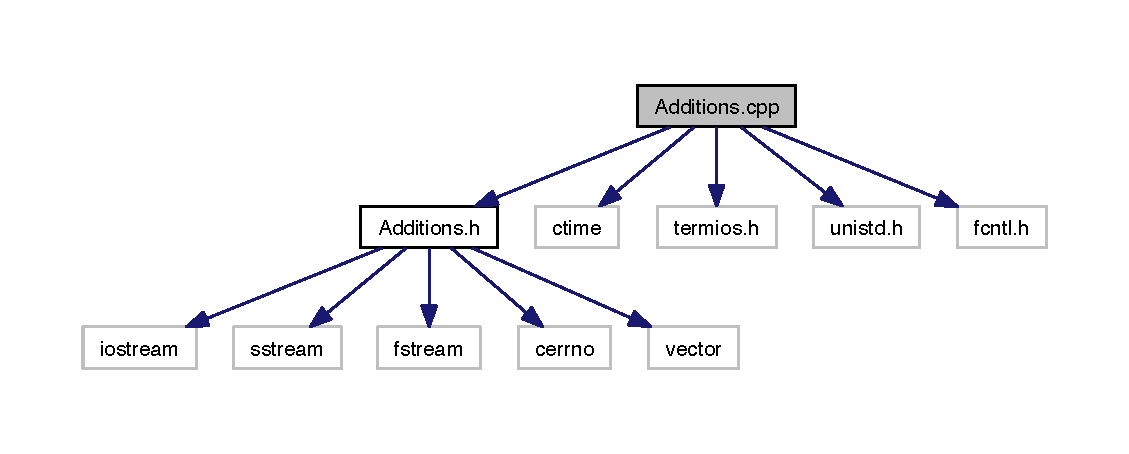
\includegraphics[width=350pt]{_additions_8cpp__incl}
\end{center}
\end{figure}
\subsection*{Namespaces}
\begin{DoxyCompactItemize}
\item 
\hyperlink{namespace_additions}{Additions}
\begin{DoxyCompactList}\small\item\em \hyperlink{namespace_additions}{Additions} namespace. \end{DoxyCompactList}\end{DoxyCompactItemize}
\subsection*{Functions}
\begin{DoxyCompactItemize}
\item 
int \hyperlink{_additions_8cpp_a27d6eaddec69251ee448adf3d7260055}{\-\_\-getch} ()
\begin{DoxyCompactList}\small\item\em Replacement \hyperlink{_additions_8cpp_a27d6eaddec69251ee448adf3d7260055}{\-\_\-getch()} for P\-O\-S\-I\-X systems. \end{DoxyCompactList}\item 
void \hyperlink{namespace_additions_a05946b8c576a8237b5b447f70e55a79d}{Additions\-::wait\-For\-Return} ()
\begin{DoxyCompactList}\small\item\em Waits until the return key is pressed. \end{DoxyCompactList}\item 
std\-::vector$<$ std\-::string $>$ \hyperlink{namespace_additions_a1abf6964ffd9abf97c743c514c2f401a}{Additions\-::explode} (const std\-::string \&delimiter, const std\-::string \&str)
\begin{DoxyCompactList}\small\item\em Converts a demlimiter-\/separated string into a vector. \end{DoxyCompactList}\item 
std\-::string \hyperlink{namespace_additions_aa81067806f9cd7e83231a302d0e4ab08}{Additions\-::get\-\_\-file\-\_\-contents} (const char $\ast$filename)
\begin{DoxyCompactList}\small\item\em Reads the content of a given file. \end{DoxyCompactList}\item 
bool \hyperlink{namespace_additions_a5dfbe44598a91e2e617b6afc56dbf6fa}{Additions\-::got\-E\-S\-C} (std\-::string str)
\begin{DoxyCompactList}\small\item\em Checks if the E\-S\-C key was pressed during a \hyperlink{namespace_additions_a9adf5327d4aa6631c5395cd58ab88237}{getline()} input. \end{DoxyCompactList}\item 
std\-::string \hyperlink{namespace_additions_a9adf5327d4aa6631c5395cd58ab88237}{Additions\-::getline} ()
\begin{DoxyCompactList}\small\item\em Reads the input from the standard input. \end{DoxyCompactList}\item 
bool \hyperlink{namespace_additions_a5b3d2c5561dcb114fbd92abc7acadc4d}{Additions\-::check\-For\-Only\-Numeric} (std\-::string str)
\begin{DoxyCompactList}\small\item\em Checks if a given string consists of numeric characters only. \end{DoxyCompactList}\item 
void \hyperlink{namespace_additions_af13c3c94d99ca27753ac564159b625d3}{Additions\-::clear\-Console} ()
\begin{DoxyCompactList}\small\item\em Clears the console. \end{DoxyCompactList}\item 
unsigned int \hyperlink{namespace_additions_a58d17107bba40cd0b819f7e595a4dd4e}{Additions\-::current\-Timestamp} ()
\begin{DoxyCompactList}\small\item\em Returns the current U\-N\-I\-X timestamp. \end{DoxyCompactList}\item 
std\-::string \hyperlink{namespace_additions_a902a81e9c6d0e2ffdd28a1f6a9d9304a}{Additions\-::timestamp\-To\-String} (const long timestamp)
\begin{DoxyCompactList}\small\item\em Converts an U\-N\-I\-X timestamp to an user-\/readable string. \end{DoxyCompactList}\end{DoxyCompactItemize}


\subsection{Function Documentation}
\hypertarget{_additions_8cpp_a27d6eaddec69251ee448adf3d7260055}{\index{Additions.\-cpp@{Additions.\-cpp}!\-\_\-getch@{\-\_\-getch}}
\index{\-\_\-getch@{\-\_\-getch}!Additions.cpp@{Additions.\-cpp}}
\subsubsection[{\-\_\-getch}]{\setlength{\rightskip}{0pt plus 5cm}int \-\_\-getch (
\begin{DoxyParamCaption}
{}
\end{DoxyParamCaption}
)}}\label{_additions_8cpp_a27d6eaddec69251ee448adf3d7260055}


Replacement \hyperlink{_additions_8cpp_a27d6eaddec69251ee448adf3d7260055}{\-\_\-getch()} for P\-O\-S\-I\-X systems. 

\begin{DoxyReturn}{Returns}
The pressed key. 
\end{DoxyReturn}

\hypertarget{_additions_8h}{\section{Additions.\-h File Reference}
\label{_additions_8h}\index{Additions.\-h@{Additions.\-h}}
}
{\ttfamily \#include $<$iostream$>$}\\*
{\ttfamily \#include $<$sstream$>$}\\*
{\ttfamily \#include $<$fstream$>$}\\*
{\ttfamily \#include $<$cerrno$>$}\\*
{\ttfamily \#include $<$vector$>$}\\*
Include dependency graph for Additions.\-h\-:
\nopagebreak
\begin{figure}[H]
\begin{center}
\leavevmode
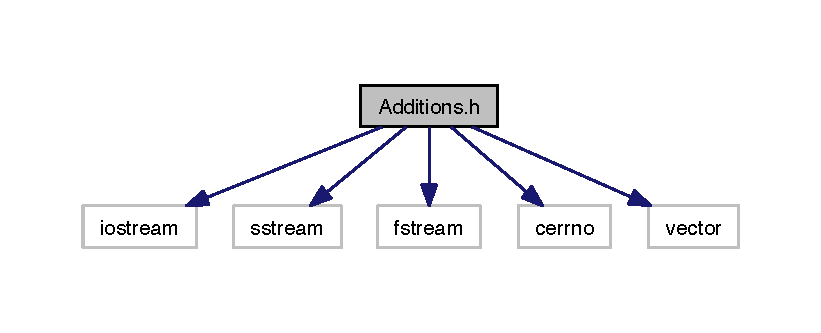
\includegraphics[width=350pt]{_additions_8h__incl}
\end{center}
\end{figure}
This graph shows which files directly or indirectly include this file\-:
\nopagebreak
\begin{figure}[H]
\begin{center}
\leavevmode
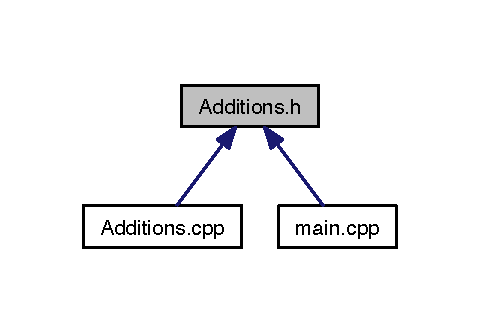
\includegraphics[width=230pt]{_additions_8h__dep__incl}
\end{center}
\end{figure}
\subsection*{Namespaces}
\begin{DoxyCompactItemize}
\item 
\hyperlink{namespace_additions}{Additions}
\begin{DoxyCompactList}\small\item\em \hyperlink{namespace_additions}{Additions} namespace. \end{DoxyCompactList}\end{DoxyCompactItemize}
\subsection*{Functions}
\begin{DoxyCompactItemize}
\item 
int \hyperlink{_additions_8h_a27d6eaddec69251ee448adf3d7260055}{\-\_\-getch} ()
\begin{DoxyCompactList}\small\item\em Replacement \hyperlink{_additions_8cpp_a27d6eaddec69251ee448adf3d7260055}{\-\_\-getch()} for P\-O\-S\-I\-X systems. \end{DoxyCompactList}\item 
std\-::vector$<$ std\-::string $>$ \hyperlink{namespace_additions_a1abf6964ffd9abf97c743c514c2f401a}{Additions\-::explode} (const std\-::string \&delimiter, const std\-::string \&str)
\begin{DoxyCompactList}\small\item\em Converts a demlimiter-\/separated string into a vector. \end{DoxyCompactList}\item 
std\-::string \hyperlink{namespace_additions_aa81067806f9cd7e83231a302d0e4ab08}{Additions\-::get\-\_\-file\-\_\-contents} (const char $\ast$filename)
\begin{DoxyCompactList}\small\item\em Reads the content of a given file. \end{DoxyCompactList}\item 
std\-::string \hyperlink{namespace_additions_a9adf5327d4aa6631c5395cd58ab88237}{Additions\-::getline} ()
\begin{DoxyCompactList}\small\item\em Reads the input from the standard input. \end{DoxyCompactList}\item 
bool \hyperlink{namespace_additions_a5b3d2c5561dcb114fbd92abc7acadc4d}{Additions\-::check\-For\-Only\-Numeric} (std\-::string str)
\begin{DoxyCompactList}\small\item\em Checks if a given string consists of numeric characters only. \end{DoxyCompactList}\item 
bool \hyperlink{namespace_additions_a5dfbe44598a91e2e617b6afc56dbf6fa}{Additions\-::got\-E\-S\-C} (std\-::string str)
\begin{DoxyCompactList}\small\item\em Checks if the E\-S\-C key was pressed during a \hyperlink{namespace_additions_a9adf5327d4aa6631c5395cd58ab88237}{getline()} input. \end{DoxyCompactList}\item 
void \hyperlink{namespace_additions_af13c3c94d99ca27753ac564159b625d3}{Additions\-::clear\-Console} ()
\begin{DoxyCompactList}\small\item\em Clears the console. \end{DoxyCompactList}\item 
void \hyperlink{namespace_additions_a05946b8c576a8237b5b447f70e55a79d}{Additions\-::wait\-For\-Return} ()
\begin{DoxyCompactList}\small\item\em Waits until the return key is pressed. \end{DoxyCompactList}\item 
unsigned int \hyperlink{namespace_additions_a58d17107bba40cd0b819f7e595a4dd4e}{Additions\-::current\-Timestamp} ()
\begin{DoxyCompactList}\small\item\em Returns the current U\-N\-I\-X timestamp. \end{DoxyCompactList}\item 
std\-::string \hyperlink{namespace_additions_a902a81e9c6d0e2ffdd28a1f6a9d9304a}{Additions\-::timestamp\-To\-String} (const long timestamp)
\begin{DoxyCompactList}\small\item\em Converts an U\-N\-I\-X timestamp to an user-\/readable string. \end{DoxyCompactList}\end{DoxyCompactItemize}


\subsection{Function Documentation}
\hypertarget{_additions_8h_a27d6eaddec69251ee448adf3d7260055}{\index{Additions.\-h@{Additions.\-h}!\-\_\-getch@{\-\_\-getch}}
\index{\-\_\-getch@{\-\_\-getch}!Additions.h@{Additions.\-h}}
\subsubsection[{\-\_\-getch}]{\setlength{\rightskip}{0pt plus 5cm}int \-\_\-getch (
\begin{DoxyParamCaption}
{}
\end{DoxyParamCaption}
)}}\label{_additions_8h_a27d6eaddec69251ee448adf3d7260055}


Replacement \hyperlink{_additions_8cpp_a27d6eaddec69251ee448adf3d7260055}{\-\_\-getch()} for P\-O\-S\-I\-X systems. 

\begin{DoxyReturn}{Returns}
The pressed key. 
\end{DoxyReturn}

\hypertarget{_database_manager_8cpp}{\section{Database\-Manager.\-cpp File Reference}
\label{_database_manager_8cpp}\index{Database\-Manager.\-cpp@{Database\-Manager.\-cpp}}
}
{\ttfamily \#include $<$fstream$>$}\\*
{\ttfamily \#include $<$boost/lexical\-\_\-cast.\-hpp$>$}\\*
{\ttfamily \#include $<$boost/algorithm/string.\-hpp$>$}\\*
{\ttfamily \#include \char`\"{}Database\-Manager.\-h\char`\"{}}\\*
{\ttfamily \#include \char`\"{}Additions.\-h\char`\"{}}\\*
Include dependency graph for Database\-Manager.\-cpp\-:
\nopagebreak
\begin{figure}[H]
\begin{center}
\leavevmode
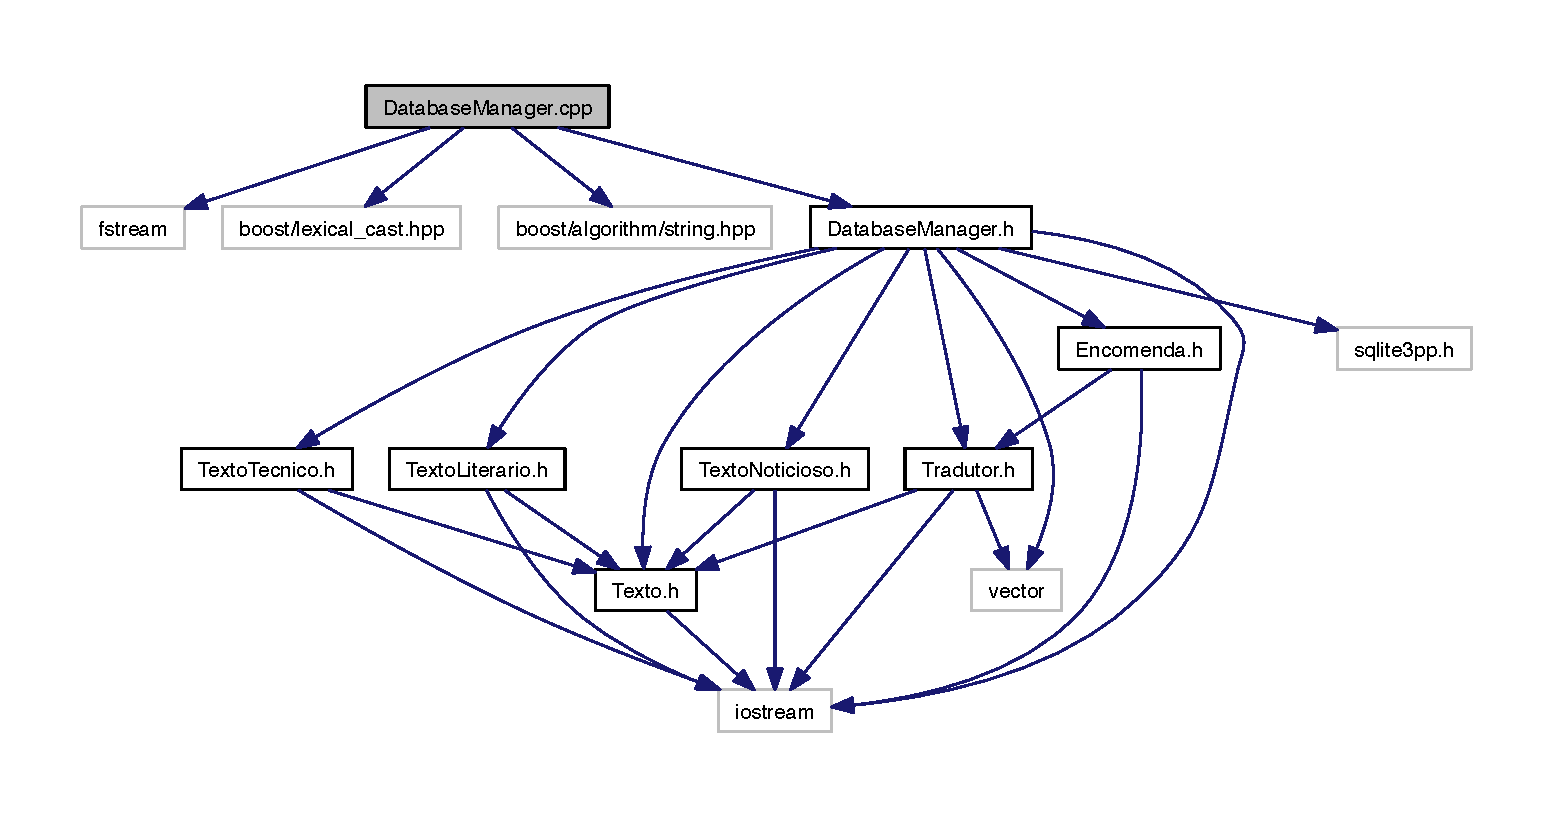
\includegraphics[width=350pt]{_database_manager_8cpp__incl}
\end{center}
\end{figure}
\subsection*{Macros}
\begin{DoxyCompactItemize}
\item 
\#define \hyperlink{_database_manager_8cpp_ad6f45b5277e7bb783bcfaed8f19388cb}{init\-\_\-db}(var)~database var(\-\_\-dbfp.\-c\-\_\-str())
\item 
\#define \hyperlink{_database_manager_8cpp_ad310b004d92e4d009daa379555ec5810}{delete\-\_\-record\-\_\-wild}(\-\_\-\-\_\-\-T\-A\-B\-L\-E\-\_\-\-N\-A\-M\-E\-\_\-\-\_\-, \-\_\-\-\_\-\-O\-B\-J\-\_\-\-N\-A\-M\-E\-\_\-\-\_\-)
\end{DoxyCompactItemize}


\subsection{Macro Definition Documentation}
\hypertarget{_database_manager_8cpp_ad310b004d92e4d009daa379555ec5810}{\index{Database\-Manager.\-cpp@{Database\-Manager.\-cpp}!delete\-\_\-record\-\_\-wild@{delete\-\_\-record\-\_\-wild}}
\index{delete\-\_\-record\-\_\-wild@{delete\-\_\-record\-\_\-wild}!DatabaseManager.cpp@{Database\-Manager.\-cpp}}
\subsubsection[{delete\-\_\-record\-\_\-wild}]{\setlength{\rightskip}{0pt plus 5cm}\#define delete\-\_\-record\-\_\-wild(
\begin{DoxyParamCaption}
\item[{}]{\-\_\-\-\_\-\-T\-A\-B\-L\-E\-\_\-\-N\-A\-M\-E\-\_\-\-\_\-, }
\item[{}]{\-\_\-\-\_\-\-O\-B\-J\-\_\-\-N\-A\-M\-E\-\_\-\-\_\-}
\end{DoxyParamCaption}
)}}\label{_database_manager_8cpp_ad310b004d92e4d009daa379555ec5810}
{\bfseries Value\-:}
\begin{DoxyCode}
\hyperlink{_database_manager_8cpp_ad6f45b5277e7bb783bcfaed8f19388cb}{init\_db}(db); \(\backslash\)
                                                            query qry(db, (std::string(\textcolor{stringliteral}{"SELECT * FROM `"}) +
       \_\_TABLE\_NAME\_\_ + std::string(\textcolor{stringliteral}{"` WHERE id="}) + boost::lexical\_cast<std::string>(\_\_OBJ\_NAME\_\_->get\_id()) + \textcolor{stringliteral}{"
       LIMIT 1"}).c\_str());    \(\backslash\)
                                                            bool exists = \textcolor{keyword}{false};    \(\backslash\)
                                                            for (query::iterator i = qry.begin(); i != qry.
      end(); ++i)  \(\backslash\)
                                                                exists = !exists;   \(\backslash\)
                                                            if (!exists)    \(\backslash\)
                                                                return \textcolor{keyword}{false};   \(\backslash\)
                                                            command cmd(db, (std::string(\textcolor{stringliteral}{"DELETE FROM `"}) +
       \_\_TABLE\_NAME\_\_ + std::string(\textcolor{stringliteral}{"` WHERE id="}) + boost::lexical\_cast<std::string>(\_\_OBJ\_NAME\_\_->get\_id())).
      c\_str());    \(\backslash\)
                                                            if (!cmd.execute()) \(\backslash\)
                                                                \textcolor{keywordflow}{return} \textcolor{keyword}{true};    \(\backslash\)
                                                            return \textcolor{keyword}{false};
\end{DoxyCode}
\hypertarget{_database_manager_8cpp_ad6f45b5277e7bb783bcfaed8f19388cb}{\index{Database\-Manager.\-cpp@{Database\-Manager.\-cpp}!init\-\_\-db@{init\-\_\-db}}
\index{init\-\_\-db@{init\-\_\-db}!DatabaseManager.cpp@{Database\-Manager.\-cpp}}
\subsubsection[{init\-\_\-db}]{\setlength{\rightskip}{0pt plus 5cm}\#define init\-\_\-db(
\begin{DoxyParamCaption}
\item[{}]{var}
\end{DoxyParamCaption}
)~database var(\-\_\-dbfp.\-c\-\_\-str())}}\label{_database_manager_8cpp_ad6f45b5277e7bb783bcfaed8f19388cb}

\hypertarget{_database_manager_8h}{\section{Database\-Manager.\-h File Reference}
\label{_database_manager_8h}\index{Database\-Manager.\-h@{Database\-Manager.\-h}}
}
{\ttfamily \#include $<$iostream$>$}\\*
{\ttfamily \#include $<$vector$>$}\\*
{\ttfamily \#include \char`\"{}sqlite3pp.\-h\char`\"{}}\\*
{\ttfamily \#include \char`\"{}Texto.\-h\char`\"{}}\\*
{\ttfamily \#include \char`\"{}Texto\-Tecnico.\-h\char`\"{}}\\*
{\ttfamily \#include \char`\"{}Texto\-Literario.\-h\char`\"{}}\\*
{\ttfamily \#include \char`\"{}Texto\-Noticioso.\-h\char`\"{}}\\*
{\ttfamily \#include \char`\"{}Tradutor.\-h\char`\"{}}\\*
{\ttfamily \#include \char`\"{}Encomenda.\-h\char`\"{}}\\*
Include dependency graph for Database\-Manager.\-h\-:
\nopagebreak
\begin{figure}[H]
\begin{center}
\leavevmode
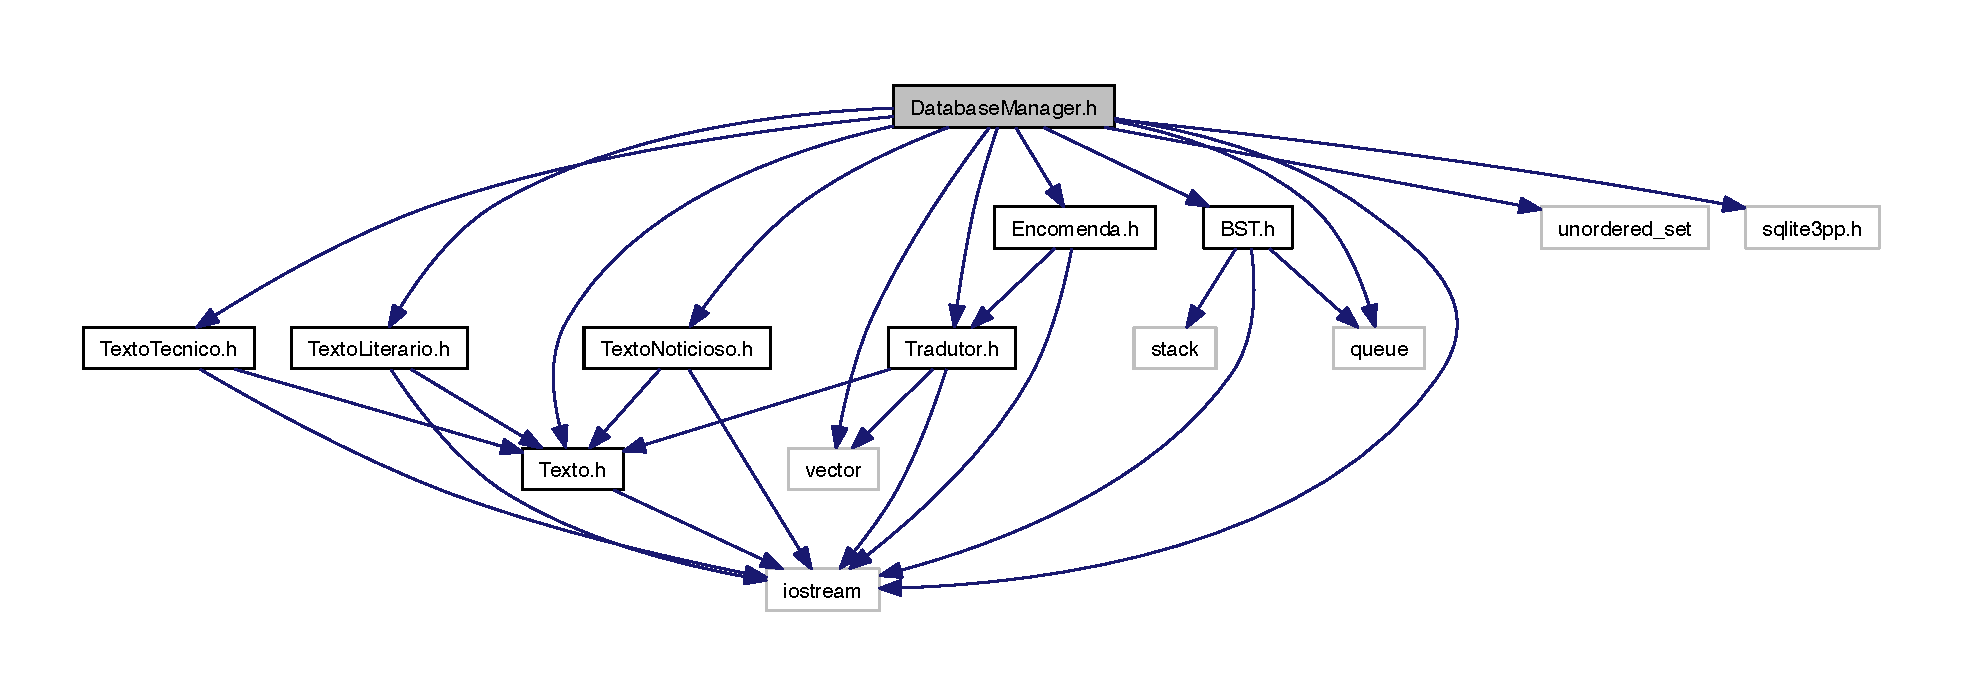
\includegraphics[width=350pt]{_database_manager_8h__incl}
\end{center}
\end{figure}
This graph shows which files directly or indirectly include this file\-:
\nopagebreak
\begin{figure}[H]
\begin{center}
\leavevmode
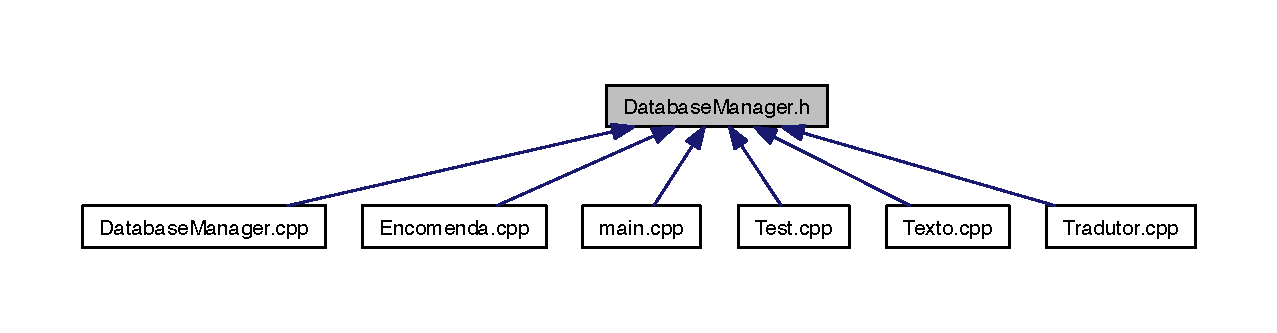
\includegraphics[width=350pt]{_database_manager_8h__dep__incl}
\end{center}
\end{figure}
\subsection*{Classes}
\begin{DoxyCompactItemize}
\item 
class \hyperlink{class_database_manager}{Database\-Manager}
\begin{DoxyCompactList}\small\item\em Database Manager class. \end{DoxyCompactList}\end{DoxyCompactItemize}
\subsection*{Enumerations}
\begin{DoxyCompactItemize}
\item 
enum \hyperlink{_database_manager_8h_afe6eaf25f136cff817dad4241aeadedb}{k\-Texto} \{ \hyperlink{_database_manager_8h_afe6eaf25f136cff817dad4241aeadedba601b6ebeb21416c7aa7e43fcd0c91564}{k\-Texto\-Base}, 
\hyperlink{_database_manager_8h_afe6eaf25f136cff817dad4241aeadedba61858b836751767e8dfd6a03b44352a9}{k\-Texto\-Tecnico}, 
\hyperlink{_database_manager_8h_afe6eaf25f136cff817dad4241aeadedbaa7596c6b206565d6f01ab2a2c60ba459}{k\-Texto\-Literario}, 
\hyperlink{_database_manager_8h_afe6eaf25f136cff817dad4241aeadedbad4c8b73ba2c61ae4e7480a3add76ecc2}{k\-Texto\-Noticioso}
 \}
\begin{DoxyCompactList}\small\item\em Text Types enum. \end{DoxyCompactList}\item 
enum \hyperlink{_database_manager_8h_ad36b2b2507c9846942e0b412d07e5438}{k\-Class} \{ \hyperlink{_database_manager_8h_ad36b2b2507c9846942e0b412d07e5438ad70eda5f7c0bfe5f9b94dcd06bc70ba1}{k\-Class\-Texto}, 
\hyperlink{_database_manager_8h_ad36b2b2507c9846942e0b412d07e5438a905951f6b0f883358810ecbd81358fae}{k\-Class\-Tradutor}, 
\hyperlink{_database_manager_8h_ad36b2b2507c9846942e0b412d07e5438a491a7f9f48558dbd59b5ee204c920bec}{k\-Class\-Encomenda}
 \}
\begin{DoxyCompactList}\small\item\em Class enum. \end{DoxyCompactList}\end{DoxyCompactItemize}


\subsection{Enumeration Type Documentation}
\hypertarget{_database_manager_8h_ad36b2b2507c9846942e0b412d07e5438}{\index{Database\-Manager.\-h@{Database\-Manager.\-h}!k\-Class@{k\-Class}}
\index{k\-Class@{k\-Class}!DatabaseManager.h@{Database\-Manager.\-h}}
\subsubsection[{k\-Class}]{\setlength{\rightskip}{0pt plus 5cm}enum {\bf k\-Class}}}\label{_database_manager_8h_ad36b2b2507c9846942e0b412d07e5438}


Class enum. 

Defines the classes as a typedef (to avoid dirty workarounds). \begin{Desc}
\item[Enumerator]\par
\begin{description}
\index{k\-Class\-Texto@{k\-Class\-Texto}!Database\-Manager.\-h@{Database\-Manager.\-h}}\index{Database\-Manager.\-h@{Database\-Manager.\-h}!k\-Class\-Texto@{k\-Class\-Texto}}\item[{\em 
\hypertarget{_database_manager_8h_ad36b2b2507c9846942e0b412d07e5438ad70eda5f7c0bfe5f9b94dcd06bc70ba1}{k\-Class\-Texto}\label{_database_manager_8h_ad36b2b2507c9846942e0b412d07e5438ad70eda5f7c0bfe5f9b94dcd06bc70ba1}
}]Class \hyperlink{class_texto}{Texto}. \index{k\-Class\-Tradutor@{k\-Class\-Tradutor}!Database\-Manager.\-h@{Database\-Manager.\-h}}\index{Database\-Manager.\-h@{Database\-Manager.\-h}!k\-Class\-Tradutor@{k\-Class\-Tradutor}}\item[{\em 
\hypertarget{_database_manager_8h_ad36b2b2507c9846942e0b412d07e5438a905951f6b0f883358810ecbd81358fae}{k\-Class\-Tradutor}\label{_database_manager_8h_ad36b2b2507c9846942e0b412d07e5438a905951f6b0f883358810ecbd81358fae}
}]Class Translator. \index{k\-Class\-Encomenda@{k\-Class\-Encomenda}!Database\-Manager.\-h@{Database\-Manager.\-h}}\index{Database\-Manager.\-h@{Database\-Manager.\-h}!k\-Class\-Encomenda@{k\-Class\-Encomenda}}\item[{\em 
\hypertarget{_database_manager_8h_ad36b2b2507c9846942e0b412d07e5438a491a7f9f48558dbd59b5ee204c920bec}{k\-Class\-Encomenda}\label{_database_manager_8h_ad36b2b2507c9846942e0b412d07e5438a491a7f9f48558dbd59b5ee204c920bec}
}]Class Order. \end{description}
\end{Desc}
\hypertarget{_database_manager_8h_afe6eaf25f136cff817dad4241aeadedb}{\index{Database\-Manager.\-h@{Database\-Manager.\-h}!k\-Texto@{k\-Texto}}
\index{k\-Texto@{k\-Texto}!DatabaseManager.h@{Database\-Manager.\-h}}
\subsubsection[{k\-Texto}]{\setlength{\rightskip}{0pt plus 5cm}enum {\bf k\-Texto}}}\label{_database_manager_8h_afe6eaf25f136cff817dad4241aeadedb}


Text Types enum. 

Defines the types of the text class as a typedef. \begin{Desc}
\item[Enumerator]\par
\begin{description}
\index{k\-Texto\-Base@{k\-Texto\-Base}!Database\-Manager.\-h@{Database\-Manager.\-h}}\index{Database\-Manager.\-h@{Database\-Manager.\-h}!k\-Texto\-Base@{k\-Texto\-Base}}\item[{\em 
\hypertarget{_database_manager_8h_afe6eaf25f136cff817dad4241aeadedba601b6ebeb21416c7aa7e43fcd0c91564}{k\-Texto\-Base}\label{_database_manager_8h_afe6eaf25f136cff817dad4241aeadedba601b6ebeb21416c7aa7e43fcd0c91564}
}]Base Text. \index{k\-Texto\-Tecnico@{k\-Texto\-Tecnico}!Database\-Manager.\-h@{Database\-Manager.\-h}}\index{Database\-Manager.\-h@{Database\-Manager.\-h}!k\-Texto\-Tecnico@{k\-Texto\-Tecnico}}\item[{\em 
\hypertarget{_database_manager_8h_afe6eaf25f136cff817dad4241aeadedba61858b836751767e8dfd6a03b44352a9}{k\-Texto\-Tecnico}\label{_database_manager_8h_afe6eaf25f136cff817dad4241aeadedba61858b836751767e8dfd6a03b44352a9}
}]Technical Text. \index{k\-Texto\-Literario@{k\-Texto\-Literario}!Database\-Manager.\-h@{Database\-Manager.\-h}}\index{Database\-Manager.\-h@{Database\-Manager.\-h}!k\-Texto\-Literario@{k\-Texto\-Literario}}\item[{\em 
\hypertarget{_database_manager_8h_afe6eaf25f136cff817dad4241aeadedbaa7596c6b206565d6f01ab2a2c60ba459}{k\-Texto\-Literario}\label{_database_manager_8h_afe6eaf25f136cff817dad4241aeadedbaa7596c6b206565d6f01ab2a2c60ba459}
}]Literary Text. \index{k\-Texto\-Noticioso@{k\-Texto\-Noticioso}!Database\-Manager.\-h@{Database\-Manager.\-h}}\index{Database\-Manager.\-h@{Database\-Manager.\-h}!k\-Texto\-Noticioso@{k\-Texto\-Noticioso}}\item[{\em 
\hypertarget{_database_manager_8h_afe6eaf25f136cff817dad4241aeadedbad4c8b73ba2c61ae4e7480a3add76ecc2}{k\-Texto\-Noticioso}\label{_database_manager_8h_afe6eaf25f136cff817dad4241aeadedbad4c8b73ba2c61ae4e7480a3add76ecc2}
}]News Text. \end{description}
\end{Desc}

\hypertarget{_encomenda_8cpp}{\section{Encomenda.\-cpp File Reference}
\label{_encomenda_8cpp}\index{Encomenda.\-cpp@{Encomenda.\-cpp}}
}
{\ttfamily \#include \char`\"{}Encomenda.\-h\char`\"{}}\\*
{\ttfamily \#include \char`\"{}Texto.\-h\char`\"{}}\\*
{\ttfamily \#include \char`\"{}Database\-Manager.\-h\char`\"{}}\\*
{\ttfamily \#include \char`\"{}Additions.\-h\char`\"{}}\\*
Include dependency graph for Encomenda.\-cpp\-:
\nopagebreak
\begin{figure}[H]
\begin{center}
\leavevmode
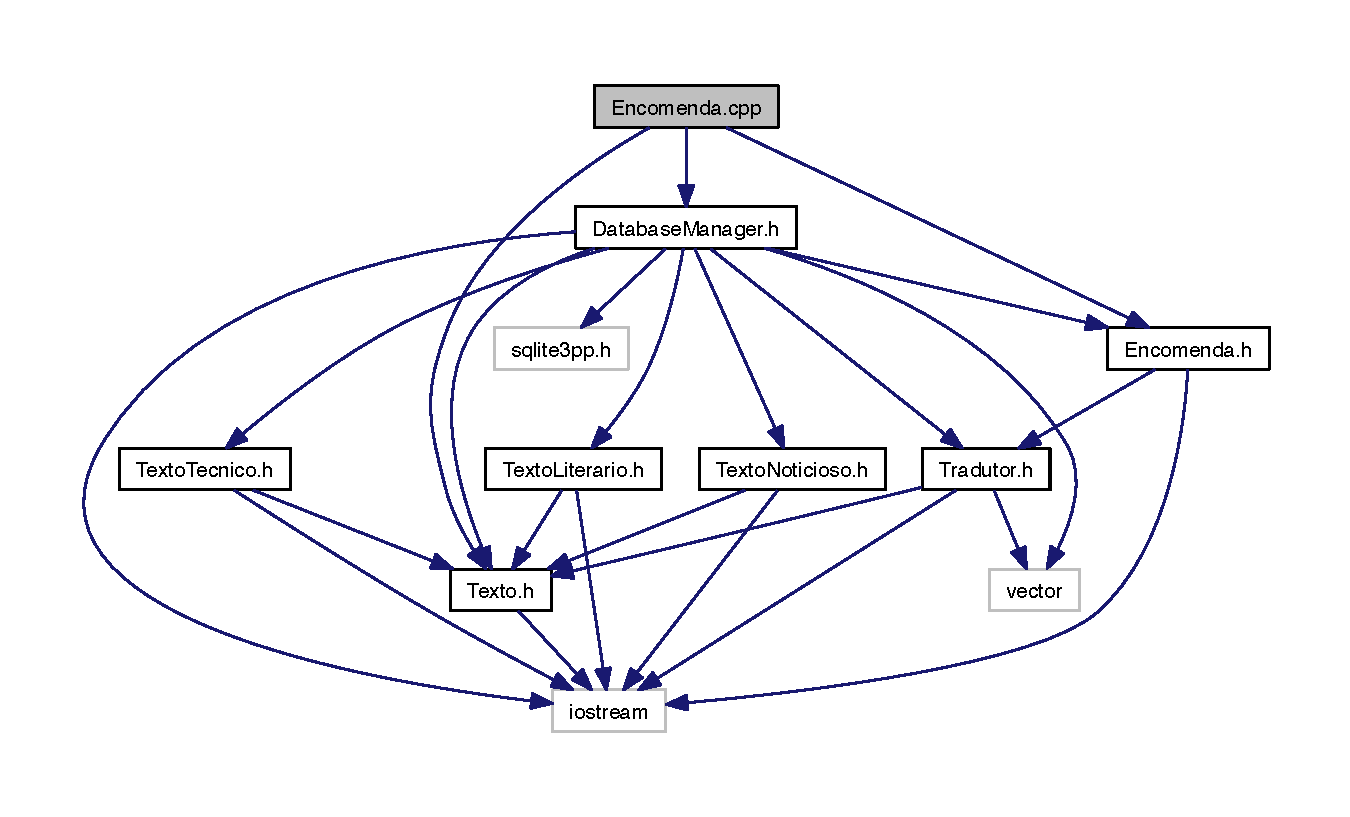
\includegraphics[width=350pt]{_encomenda_8cpp__incl}
\end{center}
\end{figure}

\hypertarget{_encomenda_8h}{\section{Encomenda.\-h File Reference}
\label{_encomenda_8h}\index{Encomenda.\-h@{Encomenda.\-h}}
}
{\ttfamily \#include $<$iostream$>$}\\*
{\ttfamily \#include \char`\"{}Tradutor.\-h\char`\"{}}\\*
Include dependency graph for Encomenda.\-h\-:
\nopagebreak
\begin{figure}[H]
\begin{center}
\leavevmode
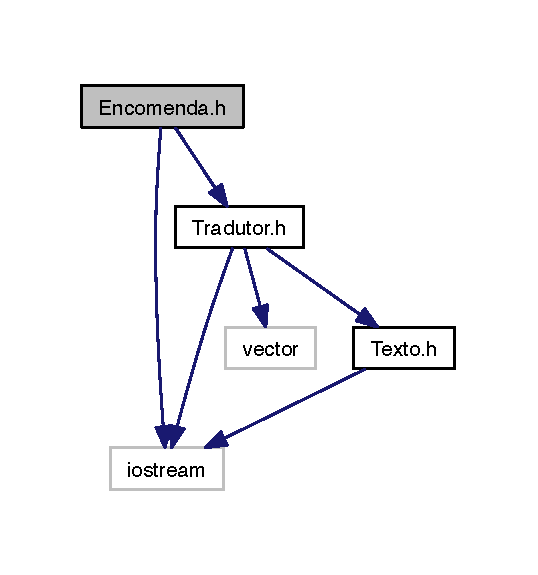
\includegraphics[width=258pt]{_encomenda_8h__incl}
\end{center}
\end{figure}
This graph shows which files directly or indirectly include this file\-:
\nopagebreak
\begin{figure}[H]
\begin{center}
\leavevmode
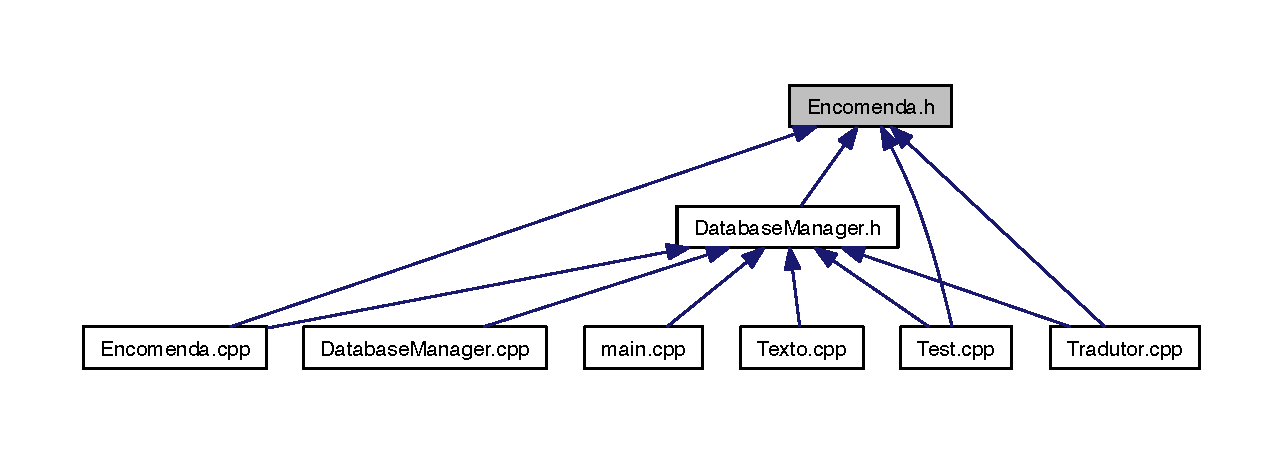
\includegraphics[width=350pt]{_encomenda_8h__dep__incl}
\end{center}
\end{figure}
\subsection*{Classes}
\begin{DoxyCompactItemize}
\item 
class \hyperlink{class_encomenda}{Encomenda}
\begin{DoxyCompactList}\small\item\em \hyperlink{class_encomenda}{Encomenda} class. \end{DoxyCompactList}\end{DoxyCompactItemize}

\hypertarget{main_8cpp}{\section{main.\-cpp File Reference}
\label{main_8cpp}\index{main.\-cpp@{main.\-cpp}}
}
{\ttfamily \#include $<$iostream$>$}\\*
{\ttfamily \#include $<$boost/lexical\-\_\-cast.\-hpp$>$}\\*
{\ttfamily \#include $<$boost/algorithm/string.\-hpp$>$}\\*
{\ttfamily \#include \char`\"{}Database\-Manager.\-h\char`\"{}}\\*
{\ttfamily \#include \char`\"{}Additions.\-h\char`\"{}}\\*
Include dependency graph for main.\-cpp\-:
\nopagebreak
\begin{figure}[H]
\begin{center}
\leavevmode
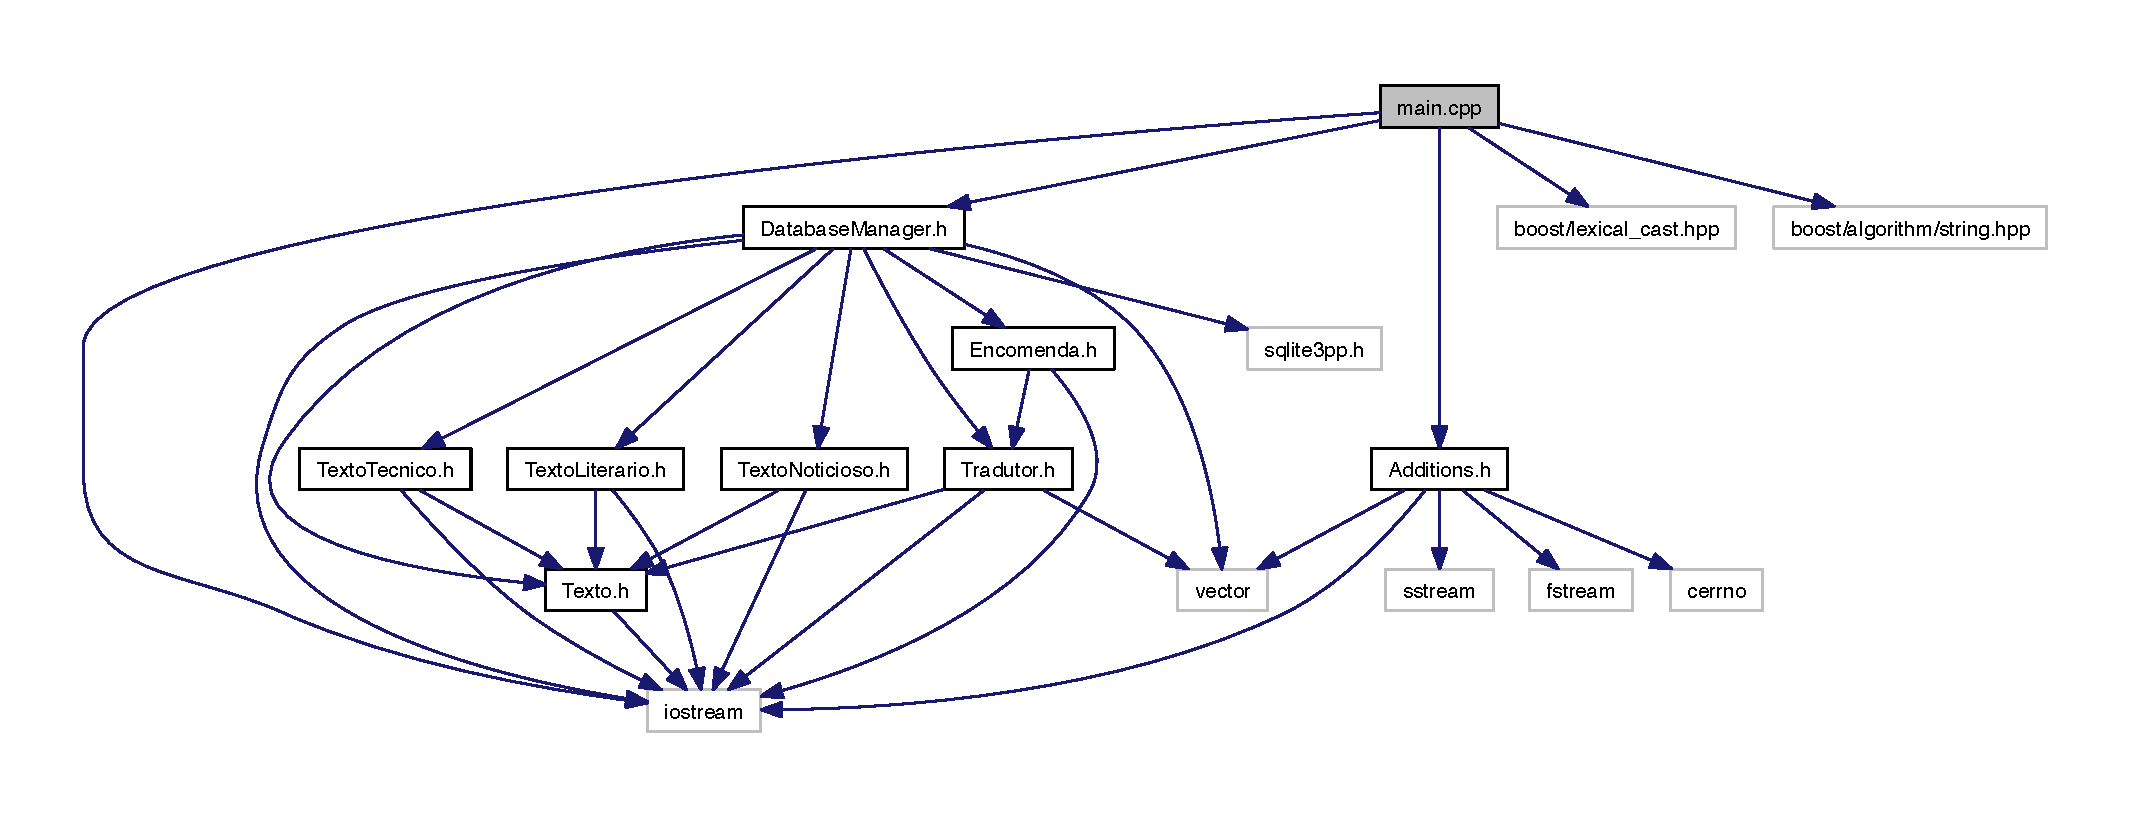
\includegraphics[width=350pt]{main_8cpp__incl}
\end{center}
\end{figure}
\subsection*{Functions}
\begin{DoxyCompactItemize}
\item 
void \hyperlink{main_8cpp_a885611589f6294afada89fe88362e863}{main\-\_\-menu} ()
\item 
void \hyperlink{main_8cpp_a531d23ea6ea2ab07c4b928afdbe779ad}{order\-\_\-translation} ()
\item 
void \hyperlink{main_8cpp_a19243f49b1bf9b191cd49f2e0a19796b}{query\-\_\-database} ()
\item 
void \hyperlink{main_8cpp_a27ad8a4d3dfbab18406f7c26c4888b44}{search\-\_\-translators} ()
\item 
void \hyperlink{main_8cpp_a263a2a48210ae4eb7df1068079f07256}{search\-\_\-orders} ()
\item 
void \hyperlink{main_8cpp_aeefb5bb46bb8d645f65495447d192fa1}{search\-\_\-texts} ()
\item 
void \hyperlink{main_8cpp_ac5074b731240b66f098ff4f158aa18bc}{search\-\_\-translators\-\_\-step2} (unsigned int search\-\_\-type)
\item 
void \hyperlink{main_8cpp_aa2e210584b9861d5f1facf9d9513ee91}{search\-\_\-orders\-\_\-step2} (unsigned int search\-\_\-type)
\item 
void \hyperlink{main_8cpp_a75f6be843294d005eccc4d2417148b40}{search\-\_\-texts\-\_\-step2} (unsigned int search\-\_\-type)
\item 
void \hyperlink{main_8cpp_a12813f39b7f720b1cd021aa125df655e}{display\-\_\-info} (\hyperlink{class_tradutor}{Tradutor} $\ast$trad)
\item 
void \hyperlink{main_8cpp_a6cbdcfe2366876365517a45b20671c84}{display\-\_\-info} (\hyperlink{class_encomenda}{Encomenda} $\ast$enc)
\item 
void \hyperlink{main_8cpp_aa1cee08b518537a6206e2bef0150b627}{display\-\_\-info} (\hyperlink{class_texto}{Texto} $\ast$txt)
\item 
void \hyperlink{main_8cpp_a4730f037ccb21250f146e3fa0a868b1c}{manage\-\_\-database} ()
\item 
void \hyperlink{main_8cpp_a43124ce79146d45230a5d96e6da92882}{add\-\_\-record} ()
\item 
void \hyperlink{main_8cpp_a246f7f8d4a33a1aed9e7030b5fb102c1}{edit\-\_\-record} ()
\item 
void \hyperlink{main_8cpp_a4791628b6e05e24fefc17e645eb6e42d}{edit\-\_\-record\-\_\-step2} (unsigned int obj\-\_\-type)
\item 
void \hyperlink{main_8cpp_a635942dacd803720a2b21b4ee18de727}{edit\-\_\-record\-\_\-step3} (\hyperlink{class_tradutor}{Tradutor} $\ast$obj)
\item 
{\footnotesize template$<$class T $>$ }\\void \hyperlink{main_8cpp_a900da0c894ff2093f906c69bc0445b31}{delete\-\_\-record\-\_\-step3} (T $\ast$obj)
\item 
int \hyperlink{main_8cpp_ac0f2228420376f4db7e1274f2b41667c}{main} (int argc, const char $\ast$argv\mbox{[}$\,$\mbox{]})
\end{DoxyCompactItemize}


\subsection{Function Documentation}
\hypertarget{main_8cpp_a43124ce79146d45230a5d96e6da92882}{\index{main.\-cpp@{main.\-cpp}!add\-\_\-record@{add\-\_\-record}}
\index{add\-\_\-record@{add\-\_\-record}!main.cpp@{main.\-cpp}}
\subsubsection[{add\-\_\-record}]{\setlength{\rightskip}{0pt plus 5cm}void add\-\_\-record (
\begin{DoxyParamCaption}
{}
\end{DoxyParamCaption}
)}}\label{main_8cpp_a43124ce79146d45230a5d96e6da92882}
\hypertarget{main_8cpp_a900da0c894ff2093f906c69bc0445b31}{\index{main.\-cpp@{main.\-cpp}!delete\-\_\-record\-\_\-step3@{delete\-\_\-record\-\_\-step3}}
\index{delete\-\_\-record\-\_\-step3@{delete\-\_\-record\-\_\-step3}!main.cpp@{main.\-cpp}}
\subsubsection[{delete\-\_\-record\-\_\-step3}]{\setlength{\rightskip}{0pt plus 5cm}template$<$class T $>$ void delete\-\_\-record\-\_\-step3 (
\begin{DoxyParamCaption}
\item[{T $\ast$}]{obj}
\end{DoxyParamCaption}
)}}\label{main_8cpp_a900da0c894ff2093f906c69bc0445b31}
\hypertarget{main_8cpp_a12813f39b7f720b1cd021aa125df655e}{\index{main.\-cpp@{main.\-cpp}!display\-\_\-info@{display\-\_\-info}}
\index{display\-\_\-info@{display\-\_\-info}!main.cpp@{main.\-cpp}}
\subsubsection[{display\-\_\-info}]{\setlength{\rightskip}{0pt plus 5cm}void display\-\_\-info (
\begin{DoxyParamCaption}
\item[{{\bf Tradutor} $\ast$}]{trad}
\end{DoxyParamCaption}
)}}\label{main_8cpp_a12813f39b7f720b1cd021aa125df655e}
\hypertarget{main_8cpp_a6cbdcfe2366876365517a45b20671c84}{\index{main.\-cpp@{main.\-cpp}!display\-\_\-info@{display\-\_\-info}}
\index{display\-\_\-info@{display\-\_\-info}!main.cpp@{main.\-cpp}}
\subsubsection[{display\-\_\-info}]{\setlength{\rightskip}{0pt plus 5cm}void display\-\_\-info (
\begin{DoxyParamCaption}
\item[{{\bf Encomenda} $\ast$}]{enc}
\end{DoxyParamCaption}
)}}\label{main_8cpp_a6cbdcfe2366876365517a45b20671c84}
\hypertarget{main_8cpp_aa1cee08b518537a6206e2bef0150b627}{\index{main.\-cpp@{main.\-cpp}!display\-\_\-info@{display\-\_\-info}}
\index{display\-\_\-info@{display\-\_\-info}!main.cpp@{main.\-cpp}}
\subsubsection[{display\-\_\-info}]{\setlength{\rightskip}{0pt plus 5cm}void display\-\_\-info (
\begin{DoxyParamCaption}
\item[{{\bf Texto} $\ast$}]{txt}
\end{DoxyParamCaption}
)}}\label{main_8cpp_aa1cee08b518537a6206e2bef0150b627}
\hypertarget{main_8cpp_a246f7f8d4a33a1aed9e7030b5fb102c1}{\index{main.\-cpp@{main.\-cpp}!edit\-\_\-record@{edit\-\_\-record}}
\index{edit\-\_\-record@{edit\-\_\-record}!main.cpp@{main.\-cpp}}
\subsubsection[{edit\-\_\-record}]{\setlength{\rightskip}{0pt plus 5cm}void edit\-\_\-record (
\begin{DoxyParamCaption}
{}
\end{DoxyParamCaption}
)}}\label{main_8cpp_a246f7f8d4a33a1aed9e7030b5fb102c1}
\hypertarget{main_8cpp_a4791628b6e05e24fefc17e645eb6e42d}{\index{main.\-cpp@{main.\-cpp}!edit\-\_\-record\-\_\-step2@{edit\-\_\-record\-\_\-step2}}
\index{edit\-\_\-record\-\_\-step2@{edit\-\_\-record\-\_\-step2}!main.cpp@{main.\-cpp}}
\subsubsection[{edit\-\_\-record\-\_\-step2}]{\setlength{\rightskip}{0pt plus 5cm}void edit\-\_\-record\-\_\-step2 (
\begin{DoxyParamCaption}
\item[{unsigned int}]{obj\-\_\-type}
\end{DoxyParamCaption}
)}}\label{main_8cpp_a4791628b6e05e24fefc17e645eb6e42d}
\hypertarget{main_8cpp_a635942dacd803720a2b21b4ee18de727}{\index{main.\-cpp@{main.\-cpp}!edit\-\_\-record\-\_\-step3@{edit\-\_\-record\-\_\-step3}}
\index{edit\-\_\-record\-\_\-step3@{edit\-\_\-record\-\_\-step3}!main.cpp@{main.\-cpp}}
\subsubsection[{edit\-\_\-record\-\_\-step3}]{\setlength{\rightskip}{0pt plus 5cm}void edit\-\_\-record\-\_\-step3 (
\begin{DoxyParamCaption}
\item[{{\bf Tradutor} $\ast$}]{obj}
\end{DoxyParamCaption}
)}}\label{main_8cpp_a635942dacd803720a2b21b4ee18de727}
\hypertarget{main_8cpp_ac0f2228420376f4db7e1274f2b41667c}{\index{main.\-cpp@{main.\-cpp}!main@{main}}
\index{main@{main}!main.cpp@{main.\-cpp}}
\subsubsection[{main}]{\setlength{\rightskip}{0pt plus 5cm}int main (
\begin{DoxyParamCaption}
\item[{int}]{argc, }
\item[{const char $\ast$}]{argv\mbox{[}$\,$\mbox{]}}
\end{DoxyParamCaption}
)}}\label{main_8cpp_ac0f2228420376f4db7e1274f2b41667c}
\hypertarget{main_8cpp_a885611589f6294afada89fe88362e863}{\index{main.\-cpp@{main.\-cpp}!main\-\_\-menu@{main\-\_\-menu}}
\index{main\-\_\-menu@{main\-\_\-menu}!main.cpp@{main.\-cpp}}
\subsubsection[{main\-\_\-menu}]{\setlength{\rightskip}{0pt plus 5cm}void main\-\_\-menu (
\begin{DoxyParamCaption}
{}
\end{DoxyParamCaption}
)}}\label{main_8cpp_a885611589f6294afada89fe88362e863}
\hypertarget{main_8cpp_a4730f037ccb21250f146e3fa0a868b1c}{\index{main.\-cpp@{main.\-cpp}!manage\-\_\-database@{manage\-\_\-database}}
\index{manage\-\_\-database@{manage\-\_\-database}!main.cpp@{main.\-cpp}}
\subsubsection[{manage\-\_\-database}]{\setlength{\rightskip}{0pt plus 5cm}void manage\-\_\-database (
\begin{DoxyParamCaption}
{}
\end{DoxyParamCaption}
)}}\label{main_8cpp_a4730f037ccb21250f146e3fa0a868b1c}
\hypertarget{main_8cpp_a531d23ea6ea2ab07c4b928afdbe779ad}{\index{main.\-cpp@{main.\-cpp}!order\-\_\-translation@{order\-\_\-translation}}
\index{order\-\_\-translation@{order\-\_\-translation}!main.cpp@{main.\-cpp}}
\subsubsection[{order\-\_\-translation}]{\setlength{\rightskip}{0pt plus 5cm}void order\-\_\-translation (
\begin{DoxyParamCaption}
{}
\end{DoxyParamCaption}
)}}\label{main_8cpp_a531d23ea6ea2ab07c4b928afdbe779ad}
\hypertarget{main_8cpp_a19243f49b1bf9b191cd49f2e0a19796b}{\index{main.\-cpp@{main.\-cpp}!query\-\_\-database@{query\-\_\-database}}
\index{query\-\_\-database@{query\-\_\-database}!main.cpp@{main.\-cpp}}
\subsubsection[{query\-\_\-database}]{\setlength{\rightskip}{0pt plus 5cm}void query\-\_\-database (
\begin{DoxyParamCaption}
{}
\end{DoxyParamCaption}
)}}\label{main_8cpp_a19243f49b1bf9b191cd49f2e0a19796b}
\hypertarget{main_8cpp_a263a2a48210ae4eb7df1068079f07256}{\index{main.\-cpp@{main.\-cpp}!search\-\_\-orders@{search\-\_\-orders}}
\index{search\-\_\-orders@{search\-\_\-orders}!main.cpp@{main.\-cpp}}
\subsubsection[{search\-\_\-orders}]{\setlength{\rightskip}{0pt plus 5cm}void search\-\_\-orders (
\begin{DoxyParamCaption}
{}
\end{DoxyParamCaption}
)}}\label{main_8cpp_a263a2a48210ae4eb7df1068079f07256}
\hypertarget{main_8cpp_aa2e210584b9861d5f1facf9d9513ee91}{\index{main.\-cpp@{main.\-cpp}!search\-\_\-orders\-\_\-step2@{search\-\_\-orders\-\_\-step2}}
\index{search\-\_\-orders\-\_\-step2@{search\-\_\-orders\-\_\-step2}!main.cpp@{main.\-cpp}}
\subsubsection[{search\-\_\-orders\-\_\-step2}]{\setlength{\rightskip}{0pt plus 5cm}void search\-\_\-orders\-\_\-step2 (
\begin{DoxyParamCaption}
\item[{unsigned int}]{search\-\_\-type}
\end{DoxyParamCaption}
)}}\label{main_8cpp_aa2e210584b9861d5f1facf9d9513ee91}
\hypertarget{main_8cpp_aeefb5bb46bb8d645f65495447d192fa1}{\index{main.\-cpp@{main.\-cpp}!search\-\_\-texts@{search\-\_\-texts}}
\index{search\-\_\-texts@{search\-\_\-texts}!main.cpp@{main.\-cpp}}
\subsubsection[{search\-\_\-texts}]{\setlength{\rightskip}{0pt plus 5cm}void search\-\_\-texts (
\begin{DoxyParamCaption}
{}
\end{DoxyParamCaption}
)}}\label{main_8cpp_aeefb5bb46bb8d645f65495447d192fa1}
\hypertarget{main_8cpp_a75f6be843294d005eccc4d2417148b40}{\index{main.\-cpp@{main.\-cpp}!search\-\_\-texts\-\_\-step2@{search\-\_\-texts\-\_\-step2}}
\index{search\-\_\-texts\-\_\-step2@{search\-\_\-texts\-\_\-step2}!main.cpp@{main.\-cpp}}
\subsubsection[{search\-\_\-texts\-\_\-step2}]{\setlength{\rightskip}{0pt plus 5cm}void search\-\_\-texts\-\_\-step2 (
\begin{DoxyParamCaption}
\item[{unsigned int}]{search\-\_\-type}
\end{DoxyParamCaption}
)}}\label{main_8cpp_a75f6be843294d005eccc4d2417148b40}
\hypertarget{main_8cpp_a27ad8a4d3dfbab18406f7c26c4888b44}{\index{main.\-cpp@{main.\-cpp}!search\-\_\-translators@{search\-\_\-translators}}
\index{search\-\_\-translators@{search\-\_\-translators}!main.cpp@{main.\-cpp}}
\subsubsection[{search\-\_\-translators}]{\setlength{\rightskip}{0pt plus 5cm}void search\-\_\-translators (
\begin{DoxyParamCaption}
{}
\end{DoxyParamCaption}
)}}\label{main_8cpp_a27ad8a4d3dfbab18406f7c26c4888b44}
\hypertarget{main_8cpp_ac5074b731240b66f098ff4f158aa18bc}{\index{main.\-cpp@{main.\-cpp}!search\-\_\-translators\-\_\-step2@{search\-\_\-translators\-\_\-step2}}
\index{search\-\_\-translators\-\_\-step2@{search\-\_\-translators\-\_\-step2}!main.cpp@{main.\-cpp}}
\subsubsection[{search\-\_\-translators\-\_\-step2}]{\setlength{\rightskip}{0pt plus 5cm}void search\-\_\-translators\-\_\-step2 (
\begin{DoxyParamCaption}
\item[{unsigned int}]{search\-\_\-type}
\end{DoxyParamCaption}
)}}\label{main_8cpp_ac5074b731240b66f098ff4f158aa18bc}

\hypertarget{_test_8cpp}{\section{Test.\-cpp File Reference}
\label{_test_8cpp}\index{Test.\-cpp@{Test.\-cpp}}
}
{\ttfamily \#include \char`\"{}cute.\-h\char`\"{}}\\*
{\ttfamily \#include \char`\"{}ide\-\_\-listener.\-h\char`\"{}}\\*
{\ttfamily \#include \char`\"{}cute\-\_\-runner.\-h\char`\"{}}\\*
{\ttfamily \#include \char`\"{}Encomenda.\-h\char`\"{}}\\*
{\ttfamily \#include \char`\"{}Texto.\-h\char`\"{}}\\*
{\ttfamily \#include \char`\"{}Texto\-Literario.\-h\char`\"{}}\\*
{\ttfamily \#include \char`\"{}Database\-Manager.\-h\char`\"{}}\\*
Include dependency graph for Test.\-cpp\-:
\nopagebreak
\begin{figure}[H]
\begin{center}
\leavevmode
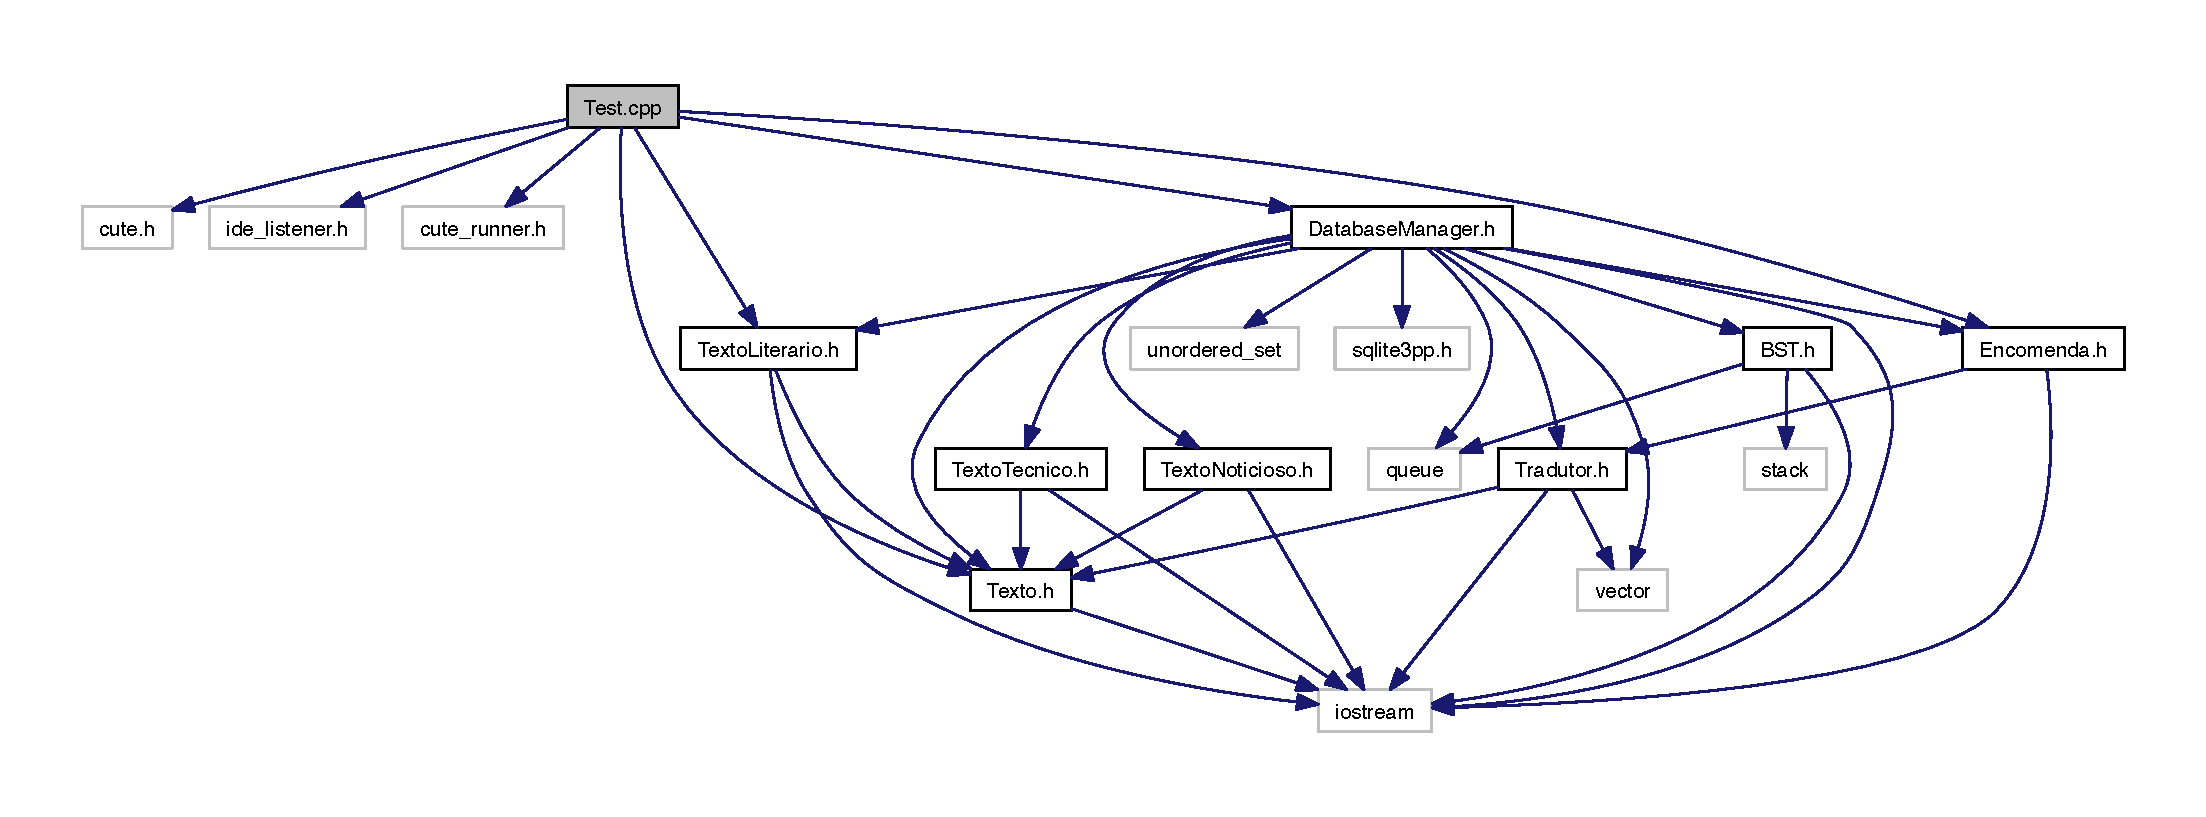
\includegraphics[width=350pt]{_test_8cpp__incl}
\end{center}
\end{figure}
\subsection*{Functions}
\begin{DoxyCompactItemize}
\item 
void \hyperlink{_test_8cpp_aafa15dfcaa7cb1f01f1cf4ed3fa0bb57}{test\-\_\-0\-\_\-wordcount} ()
\item 
void \hyperlink{_test_8cpp_ab64d91fc243933014fe89d33cbae297d}{test\-\_\-1\-\_\-create} ()
\item 
void \hyperlink{_test_8cpp_a054d5b63cc8bc739206e9df16c3f771b}{test\-\_\-2\-\_\-load} ()
\item 
void \hyperlink{_test_8cpp_a2e810ad64864ec3baa715234093f3e8b}{test\-\_\-3\-\_\-update} ()
\item 
void \hyperlink{_test_8cpp_a5b87bc2e2a7cfae16d5ceeab78e0dd3b}{run\-\_\-test\-\_\-suite} ()
\end{DoxyCompactItemize}


\subsection{Function Documentation}
\hypertarget{_test_8cpp_a5b87bc2e2a7cfae16d5ceeab78e0dd3b}{\index{Test.\-cpp@{Test.\-cpp}!run\-\_\-test\-\_\-suite@{run\-\_\-test\-\_\-suite}}
\index{run\-\_\-test\-\_\-suite@{run\-\_\-test\-\_\-suite}!Test.cpp@{Test.\-cpp}}
\subsubsection[{run\-\_\-test\-\_\-suite}]{\setlength{\rightskip}{0pt plus 5cm}void run\-\_\-test\-\_\-suite (
\begin{DoxyParamCaption}
{}
\end{DoxyParamCaption}
)}}\label{_test_8cpp_a5b87bc2e2a7cfae16d5ceeab78e0dd3b}
\hypertarget{_test_8cpp_aafa15dfcaa7cb1f01f1cf4ed3fa0bb57}{\index{Test.\-cpp@{Test.\-cpp}!test\-\_\-0\-\_\-wordcount@{test\-\_\-0\-\_\-wordcount}}
\index{test\-\_\-0\-\_\-wordcount@{test\-\_\-0\-\_\-wordcount}!Test.cpp@{Test.\-cpp}}
\subsubsection[{test\-\_\-0\-\_\-wordcount}]{\setlength{\rightskip}{0pt plus 5cm}void test\-\_\-0\-\_\-wordcount (
\begin{DoxyParamCaption}
{}
\end{DoxyParamCaption}
)}}\label{_test_8cpp_aafa15dfcaa7cb1f01f1cf4ed3fa0bb57}
\hypertarget{_test_8cpp_ab64d91fc243933014fe89d33cbae297d}{\index{Test.\-cpp@{Test.\-cpp}!test\-\_\-1\-\_\-create@{test\-\_\-1\-\_\-create}}
\index{test\-\_\-1\-\_\-create@{test\-\_\-1\-\_\-create}!Test.cpp@{Test.\-cpp}}
\subsubsection[{test\-\_\-1\-\_\-create}]{\setlength{\rightskip}{0pt plus 5cm}void test\-\_\-1\-\_\-create (
\begin{DoxyParamCaption}
{}
\end{DoxyParamCaption}
)}}\label{_test_8cpp_ab64d91fc243933014fe89d33cbae297d}
\hypertarget{_test_8cpp_a054d5b63cc8bc739206e9df16c3f771b}{\index{Test.\-cpp@{Test.\-cpp}!test\-\_\-2\-\_\-load@{test\-\_\-2\-\_\-load}}
\index{test\-\_\-2\-\_\-load@{test\-\_\-2\-\_\-load}!Test.cpp@{Test.\-cpp}}
\subsubsection[{test\-\_\-2\-\_\-load}]{\setlength{\rightskip}{0pt plus 5cm}void test\-\_\-2\-\_\-load (
\begin{DoxyParamCaption}
{}
\end{DoxyParamCaption}
)}}\label{_test_8cpp_a054d5b63cc8bc739206e9df16c3f771b}
\hypertarget{_test_8cpp_a2e810ad64864ec3baa715234093f3e8b}{\index{Test.\-cpp@{Test.\-cpp}!test\-\_\-3\-\_\-update@{test\-\_\-3\-\_\-update}}
\index{test\-\_\-3\-\_\-update@{test\-\_\-3\-\_\-update}!Test.cpp@{Test.\-cpp}}
\subsubsection[{test\-\_\-3\-\_\-update}]{\setlength{\rightskip}{0pt plus 5cm}void test\-\_\-3\-\_\-update (
\begin{DoxyParamCaption}
{}
\end{DoxyParamCaption}
)}}\label{_test_8cpp_a2e810ad64864ec3baa715234093f3e8b}

\hypertarget{_test_8h}{\section{Test.\-h File Reference}
\label{_test_8h}\index{Test.\-h@{Test.\-h}}
}
\subsection*{Functions}
\begin{DoxyCompactItemize}
\item 
void \hyperlink{_test_8h_a5b87bc2e2a7cfae16d5ceeab78e0dd3b}{run\-\_\-test\-\_\-suite} ()
\end{DoxyCompactItemize}


\subsection{Function Documentation}
\hypertarget{_test_8h_a5b87bc2e2a7cfae16d5ceeab78e0dd3b}{\index{Test.\-h@{Test.\-h}!run\-\_\-test\-\_\-suite@{run\-\_\-test\-\_\-suite}}
\index{run\-\_\-test\-\_\-suite@{run\-\_\-test\-\_\-suite}!Test.h@{Test.\-h}}
\subsubsection[{run\-\_\-test\-\_\-suite}]{\setlength{\rightskip}{0pt plus 5cm}void run\-\_\-test\-\_\-suite (
\begin{DoxyParamCaption}
{}
\end{DoxyParamCaption}
)}}\label{_test_8h_a5b87bc2e2a7cfae16d5ceeab78e0dd3b}

\hypertarget{_texto_8cpp}{\section{Texto.\-cpp File Reference}
\label{_texto_8cpp}\index{Texto.\-cpp@{Texto.\-cpp}}
}
{\ttfamily \#include $<$sstream$>$}\\*
{\ttfamily \#include $<$vector$>$}\\*
{\ttfamily \#include $<$boost/algorithm/string.\-hpp$>$}\\*
{\ttfamily \#include \char`\"{}Texto.\-h\char`\"{}}\\*
{\ttfamily \#include \char`\"{}Database\-Manager.\-h\char`\"{}}\\*
Include dependency graph for Texto.\-cpp\-:
\nopagebreak
\begin{figure}[H]
\begin{center}
\leavevmode
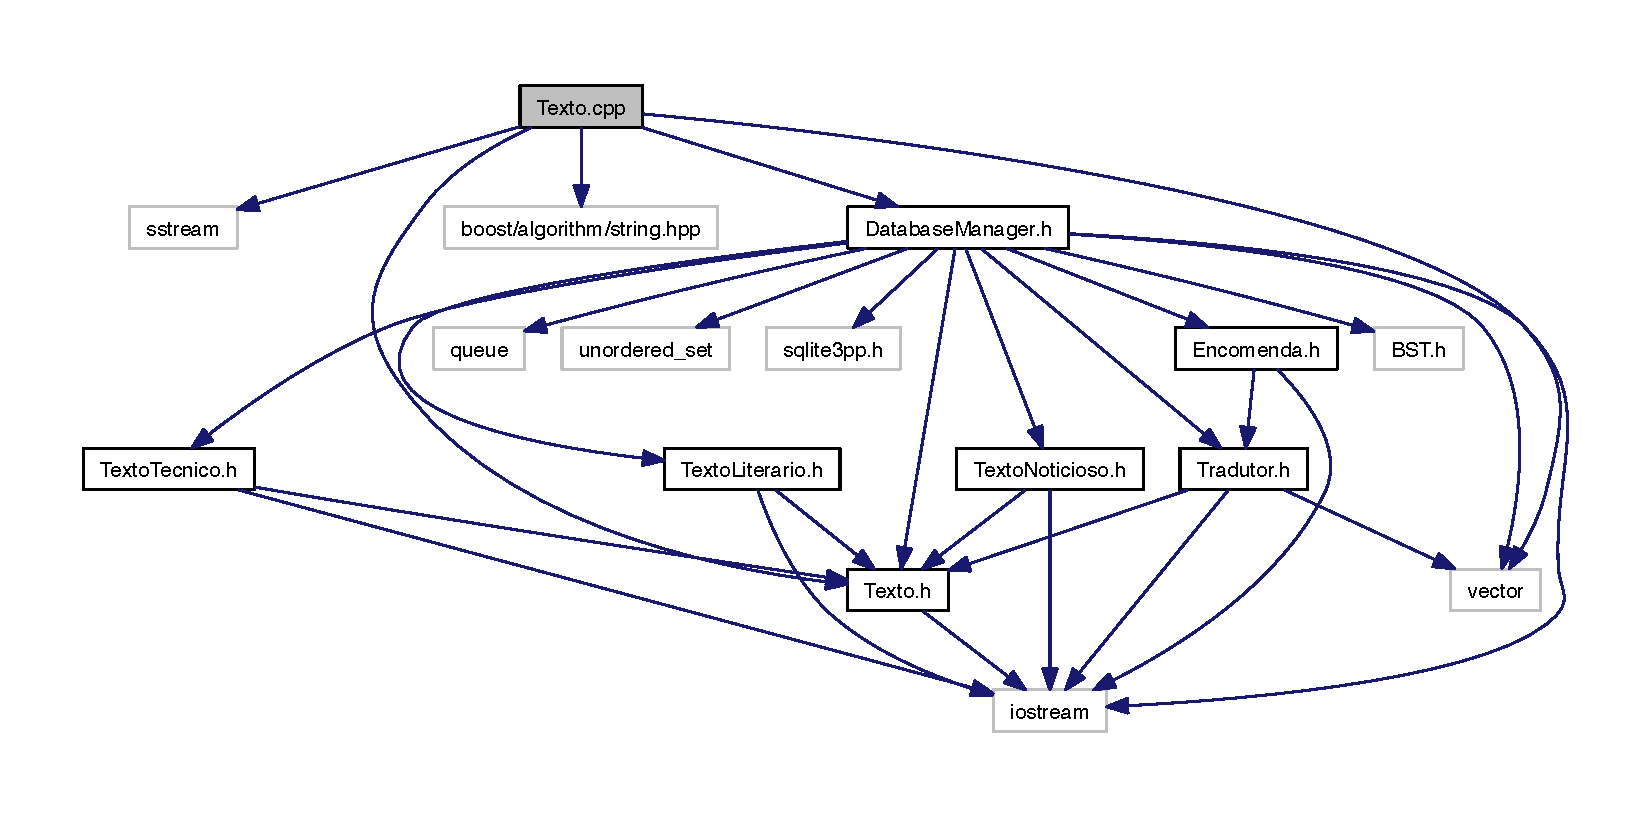
\includegraphics[width=350pt]{_texto_8cpp__incl}
\end{center}
\end{figure}
\subsection*{Macros}
\begin{DoxyCompactItemize}
\item 
\#define \hyperlink{_texto_8cpp_af7f4f864ac8909a815f7d7968aff1b4f}{W\-H\-I\-T\-E\-S\-P\-A\-C\-E\-\_\-\-E\-N\-D\-L\-I\-N\-E\-\_\-\-C\-H\-A\-R\-S}~\char`\"{} \textbackslash{}t\textbackslash{}n\textbackslash{}v\textbackslash{}f\textbackslash{}r\char`\"{}
\end{DoxyCompactItemize}


\subsection{Macro Definition Documentation}
\hypertarget{_texto_8cpp_af7f4f864ac8909a815f7d7968aff1b4f}{\index{Texto.\-cpp@{Texto.\-cpp}!W\-H\-I\-T\-E\-S\-P\-A\-C\-E\-\_\-\-E\-N\-D\-L\-I\-N\-E\-\_\-\-C\-H\-A\-R\-S@{W\-H\-I\-T\-E\-S\-P\-A\-C\-E\-\_\-\-E\-N\-D\-L\-I\-N\-E\-\_\-\-C\-H\-A\-R\-S}}
\index{W\-H\-I\-T\-E\-S\-P\-A\-C\-E\-\_\-\-E\-N\-D\-L\-I\-N\-E\-\_\-\-C\-H\-A\-R\-S@{W\-H\-I\-T\-E\-S\-P\-A\-C\-E\-\_\-\-E\-N\-D\-L\-I\-N\-E\-\_\-\-C\-H\-A\-R\-S}!Texto.cpp@{Texto.\-cpp}}
\subsubsection[{W\-H\-I\-T\-E\-S\-P\-A\-C\-E\-\_\-\-E\-N\-D\-L\-I\-N\-E\-\_\-\-C\-H\-A\-R\-S}]{\setlength{\rightskip}{0pt plus 5cm}\#define W\-H\-I\-T\-E\-S\-P\-A\-C\-E\-\_\-\-E\-N\-D\-L\-I\-N\-E\-\_\-\-C\-H\-A\-R\-S~\char`\"{} \textbackslash{}t\textbackslash{}n\textbackslash{}v\textbackslash{}f\textbackslash{}r\char`\"{}}}\label{_texto_8cpp_af7f4f864ac8909a815f7d7968aff1b4f}

\hypertarget{_texto_8h}{\section{Texto.\-h File Reference}
\label{_texto_8h}\index{Texto.\-h@{Texto.\-h}}
}
{\ttfamily \#include $<$iostream$>$}\\*
Include dependency graph for Texto.\-h\-:
\nopagebreak
\begin{figure}[H]
\begin{center}
\leavevmode
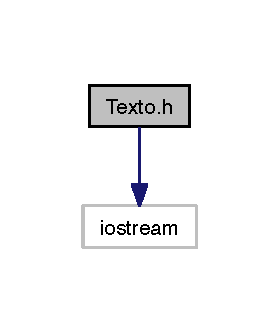
\includegraphics[width=134pt]{_texto_8h__incl}
\end{center}
\end{figure}
This graph shows which files directly or indirectly include this file\-:
\nopagebreak
\begin{figure}[H]
\begin{center}
\leavevmode
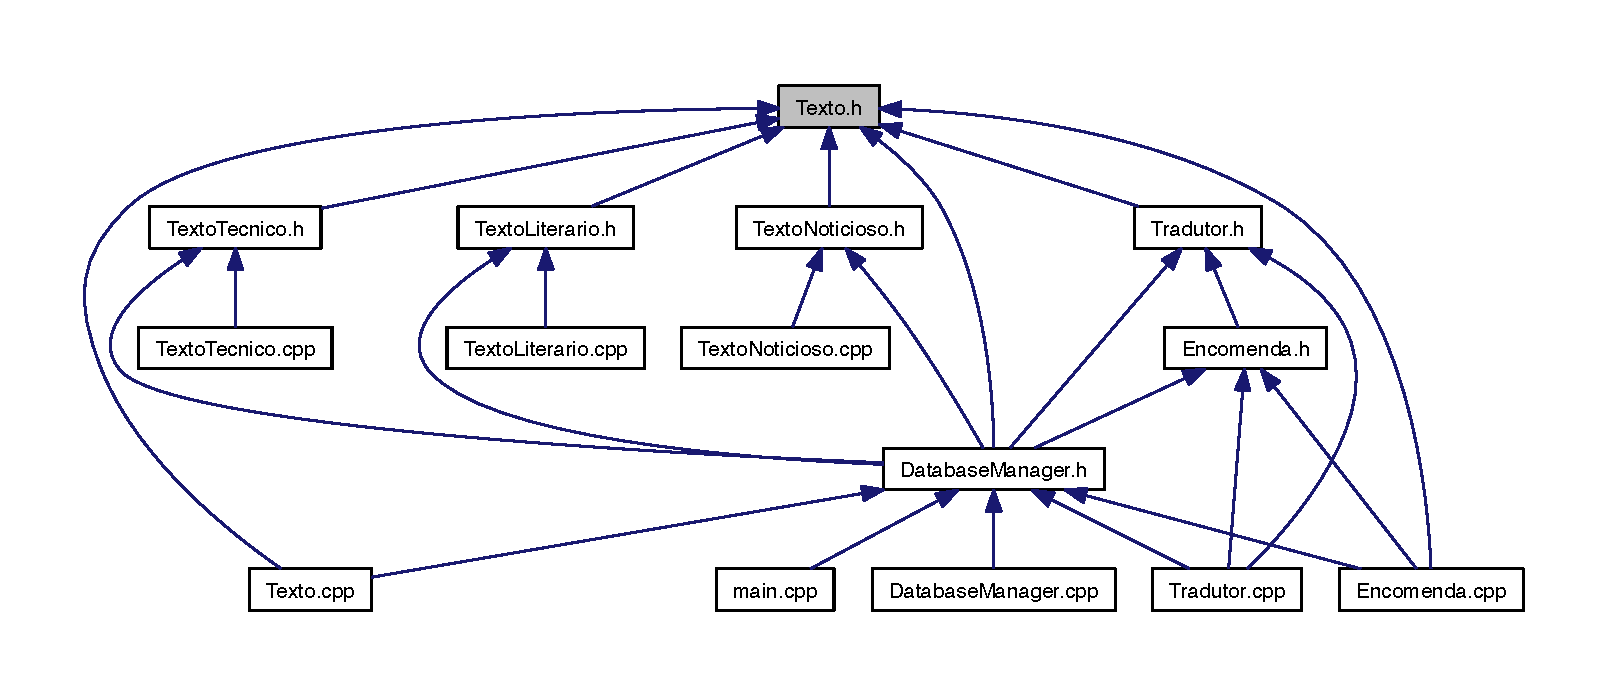
\includegraphics[width=350pt]{_texto_8h__dep__incl}
\end{center}
\end{figure}
\subsection*{Classes}
\begin{DoxyCompactItemize}
\item 
class \hyperlink{class_texto}{Texto}
\begin{DoxyCompactList}\small\item\em \hyperlink{class_texto}{Texto} /abstract/ class. \end{DoxyCompactList}\end{DoxyCompactItemize}

\hypertarget{_texto_literario_8cpp}{\section{Texto\-Literario.\-cpp File Reference}
\label{_texto_literario_8cpp}\index{Texto\-Literario.\-cpp@{Texto\-Literario.\-cpp}}
}
{\ttfamily \#include \char`\"{}Texto\-Literario.\-h\char`\"{}}\\*
Include dependency graph for Texto\-Literario.\-cpp\-:
\nopagebreak
\begin{figure}[H]
\begin{center}
\leavevmode
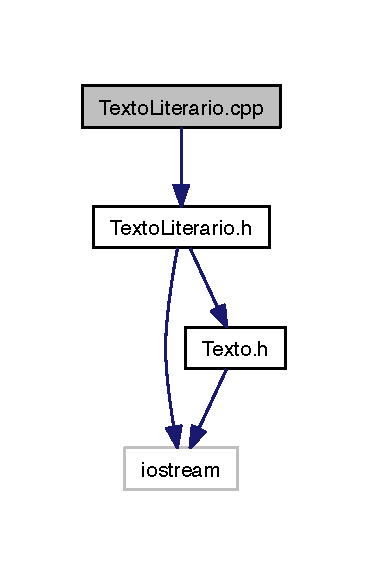
\includegraphics[width=177pt]{_texto_literario_8cpp__incl}
\end{center}
\end{figure}

\hypertarget{_texto_literario_8h}{\section{Texto\-Literario.\-h File Reference}
\label{_texto_literario_8h}\index{Texto\-Literario.\-h@{Texto\-Literario.\-h}}
}
{\ttfamily \#include $<$iostream$>$}\\*
{\ttfamily \#include \char`\"{}Texto.\-h\char`\"{}}\\*
Include dependency graph for Texto\-Literario.\-h\-:
\nopagebreak
\begin{figure}[H]
\begin{center}
\leavevmode
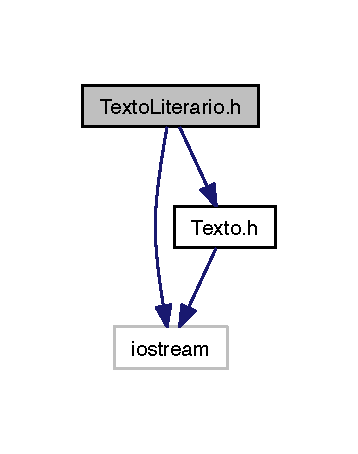
\includegraphics[width=172pt]{_texto_literario_8h__incl}
\end{center}
\end{figure}
This graph shows which files directly or indirectly include this file\-:
\nopagebreak
\begin{figure}[H]
\begin{center}
\leavevmode
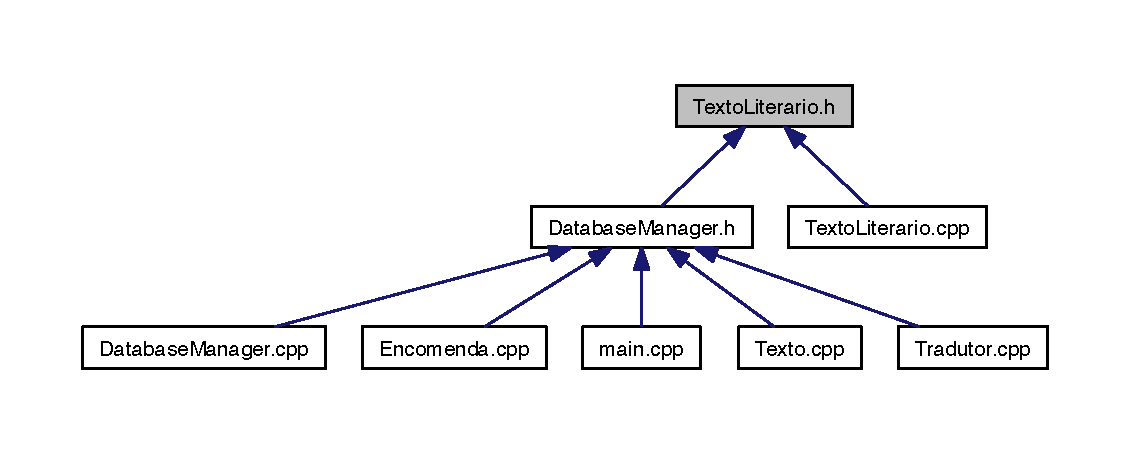
\includegraphics[width=350pt]{_texto_literario_8h__dep__incl}
\end{center}
\end{figure}
\subsection*{Classes}
\begin{DoxyCompactItemize}
\item 
class \hyperlink{class_texto_literario}{Texto\-Literario}
\begin{DoxyCompactList}\small\item\em \hyperlink{class_texto}{Texto} Literario class. \end{DoxyCompactList}\end{DoxyCompactItemize}

\hypertarget{_texto_noticioso_8cpp}{\section{Texto\-Noticioso.\-cpp File Reference}
\label{_texto_noticioso_8cpp}\index{Texto\-Noticioso.\-cpp@{Texto\-Noticioso.\-cpp}}
}
{\ttfamily \#include \char`\"{}Texto\-Noticioso.\-h\char`\"{}}\\*
Include dependency graph for Texto\-Noticioso.\-cpp\-:
\nopagebreak
\begin{figure}[H]
\begin{center}
\leavevmode
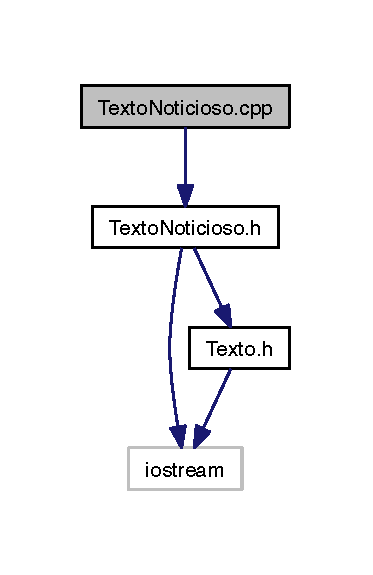
\includegraphics[width=179pt]{_texto_noticioso_8cpp__incl}
\end{center}
\end{figure}

\hypertarget{_texto_noticioso_8h}{\section{Texto\-Noticioso.\-h File Reference}
\label{_texto_noticioso_8h}\index{Texto\-Noticioso.\-h@{Texto\-Noticioso.\-h}}
}
{\ttfamily \#include $<$iostream$>$}\\*
{\ttfamily \#include \char`\"{}Texto.\-h\char`\"{}}\\*
Include dependency graph for Texto\-Noticioso.\-h\-:
\nopagebreak
\begin{figure}[H]
\begin{center}
\leavevmode
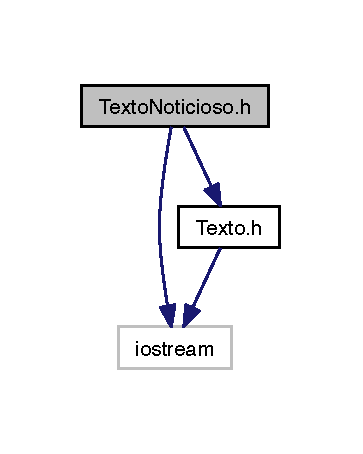
\includegraphics[width=174pt]{_texto_noticioso_8h__incl}
\end{center}
\end{figure}
This graph shows which files directly or indirectly include this file\-:
\nopagebreak
\begin{figure}[H]
\begin{center}
\leavevmode
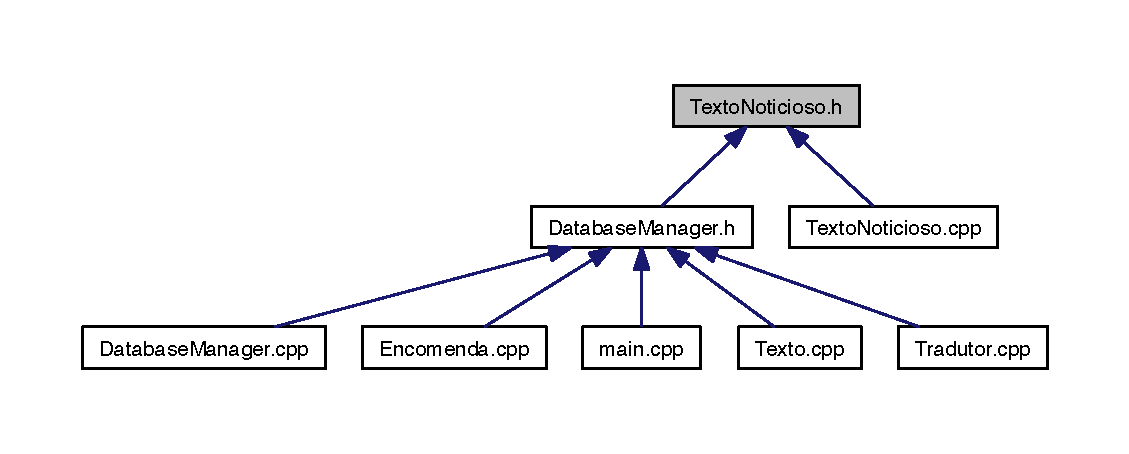
\includegraphics[width=350pt]{_texto_noticioso_8h__dep__incl}
\end{center}
\end{figure}
\subsection*{Classes}
\begin{DoxyCompactItemize}
\item 
class \hyperlink{class_texto_noticioso}{Texto\-Noticioso}
\begin{DoxyCompactList}\small\item\em \hyperlink{class_texto}{Texto} Noticioso class. \end{DoxyCompactList}\end{DoxyCompactItemize}
\subsection*{Enumerations}
\begin{DoxyCompactItemize}
\item 
enum \hyperlink{_texto_noticioso_8h_adbee2daefeb8a5b2ec0e0c0b353390d5}{tipo\-\_\-jornal} \{ \hyperlink{_texto_noticioso_8h_adbee2daefeb8a5b2ec0e0c0b353390d5ac24612edaf40d3e32051ffd6b9d5e66f}{tipo\-\_\-jornal\-\_\-diario}, 
\hyperlink{_texto_noticioso_8h_adbee2daefeb8a5b2ec0e0c0b353390d5af48430c9000475e4d945b3e7e6dba661}{tipo\-\_\-jornal\-\_\-semanario}
 \}
\end{DoxyCompactItemize}


\subsection{Enumeration Type Documentation}
\hypertarget{_texto_noticioso_8h_adbee2daefeb8a5b2ec0e0c0b353390d5}{\index{Texto\-Noticioso.\-h@{Texto\-Noticioso.\-h}!tipo\-\_\-jornal@{tipo\-\_\-jornal}}
\index{tipo\-\_\-jornal@{tipo\-\_\-jornal}!TextoNoticioso.h@{Texto\-Noticioso.\-h}}
\subsubsection[{tipo\-\_\-jornal}]{\setlength{\rightskip}{0pt plus 5cm}enum {\bf tipo\-\_\-jornal}}}\label{_texto_noticioso_8h_adbee2daefeb8a5b2ec0e0c0b353390d5}
\begin{Desc}
\item[Enumerator]\par
\begin{description}
\index{tipo\-\_\-jornal\-\_\-diario@{tipo\-\_\-jornal\-\_\-diario}!Texto\-Noticioso.\-h@{Texto\-Noticioso.\-h}}\index{Texto\-Noticioso.\-h@{Texto\-Noticioso.\-h}!tipo\-\_\-jornal\-\_\-diario@{tipo\-\_\-jornal\-\_\-diario}}\item[{\em 
\hypertarget{_texto_noticioso_8h_adbee2daefeb8a5b2ec0e0c0b353390d5ac24612edaf40d3e32051ffd6b9d5e66f}{tipo\-\_\-jornal\-\_\-diario}\label{_texto_noticioso_8h_adbee2daefeb8a5b2ec0e0c0b353390d5ac24612edaf40d3e32051ffd6b9d5e66f}
}]\index{tipo\-\_\-jornal\-\_\-semanario@{tipo\-\_\-jornal\-\_\-semanario}!Texto\-Noticioso.\-h@{Texto\-Noticioso.\-h}}\index{Texto\-Noticioso.\-h@{Texto\-Noticioso.\-h}!tipo\-\_\-jornal\-\_\-semanario@{tipo\-\_\-jornal\-\_\-semanario}}\item[{\em 
\hypertarget{_texto_noticioso_8h_adbee2daefeb8a5b2ec0e0c0b353390d5af48430c9000475e4d945b3e7e6dba661}{tipo\-\_\-jornal\-\_\-semanario}\label{_texto_noticioso_8h_adbee2daefeb8a5b2ec0e0c0b353390d5af48430c9000475e4d945b3e7e6dba661}
}]\end{description}
\end{Desc}

\hypertarget{_texto_tecnico_8cpp}{\section{Texto\-Tecnico.\-cpp File Reference}
\label{_texto_tecnico_8cpp}\index{Texto\-Tecnico.\-cpp@{Texto\-Tecnico.\-cpp}}
}
{\ttfamily \#include \char`\"{}Texto\-Tecnico.\-h\char`\"{}}\\*
Include dependency graph for Texto\-Tecnico.\-cpp\-:
\nopagebreak
\begin{figure}[H]
\begin{center}
\leavevmode
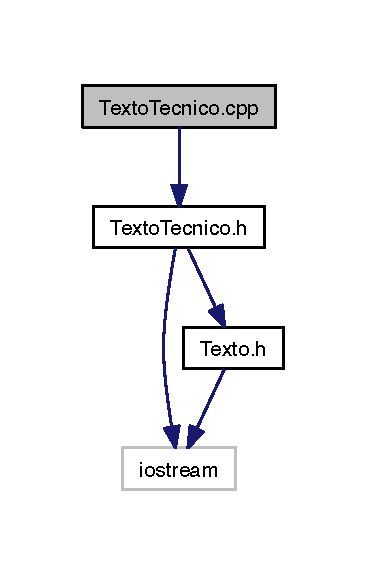
\includegraphics[width=176pt]{_texto_tecnico_8cpp__incl}
\end{center}
\end{figure}

\hypertarget{_texto_tecnico_8h}{\section{Texto\-Tecnico.\-h File Reference}
\label{_texto_tecnico_8h}\index{Texto\-Tecnico.\-h@{Texto\-Tecnico.\-h}}
}
{\ttfamily \#include $<$iostream$>$}\\*
{\ttfamily \#include \char`\"{}Texto.\-h\char`\"{}}\\*
Include dependency graph for Texto\-Tecnico.\-h\-:
\nopagebreak
\begin{figure}[H]
\begin{center}
\leavevmode
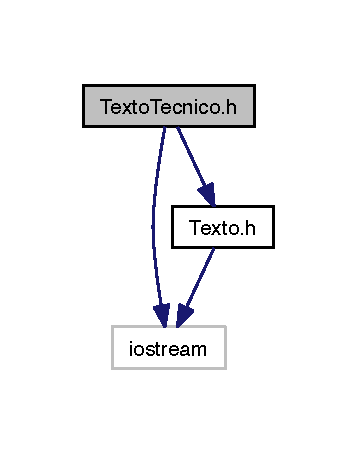
\includegraphics[width=171pt]{_texto_tecnico_8h__incl}
\end{center}
\end{figure}
This graph shows which files directly or indirectly include this file\-:
\nopagebreak
\begin{figure}[H]
\begin{center}
\leavevmode
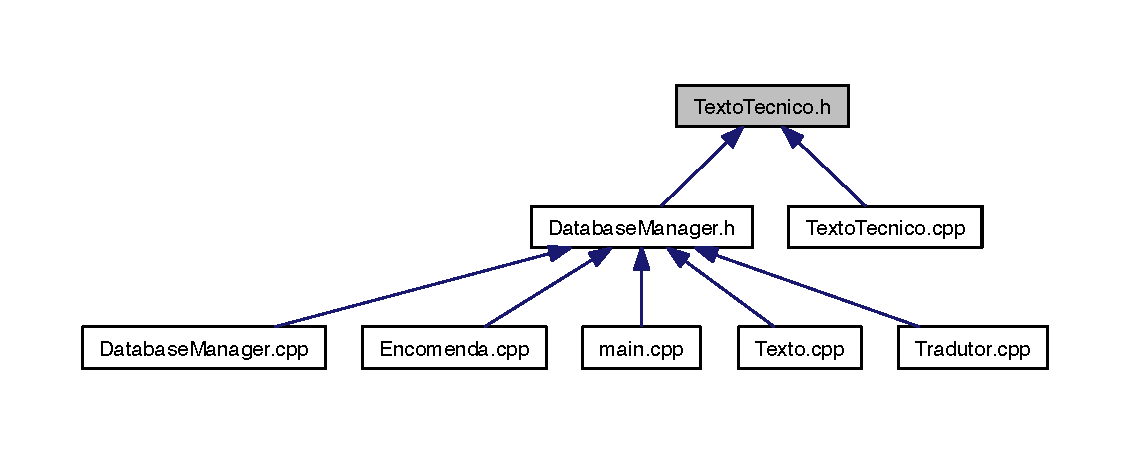
\includegraphics[width=350pt]{_texto_tecnico_8h__dep__incl}
\end{center}
\end{figure}
\subsection*{Classes}
\begin{DoxyCompactItemize}
\item 
class \hyperlink{class_texto_tecnico}{Texto\-Tecnico}
\begin{DoxyCompactList}\small\item\em \hyperlink{class_texto}{Texto} Tecnico class. \end{DoxyCompactList}\end{DoxyCompactItemize}

\hypertarget{_tradutor_8cpp}{\section{Tradutor.\-cpp File Reference}
\label{_tradutor_8cpp}\index{Tradutor.\-cpp@{Tradutor.\-cpp}}
}
{\ttfamily \#include \char`\"{}Tradutor.\-h\char`\"{}}\\*
{\ttfamily \#include \char`\"{}Encomenda.\-h\char`\"{}}\\*
{\ttfamily \#include \char`\"{}Database\-Manager.\-h\char`\"{}}\\*
Include dependency graph for Tradutor.\-cpp\-:
\nopagebreak
\begin{figure}[H]
\begin{center}
\leavevmode
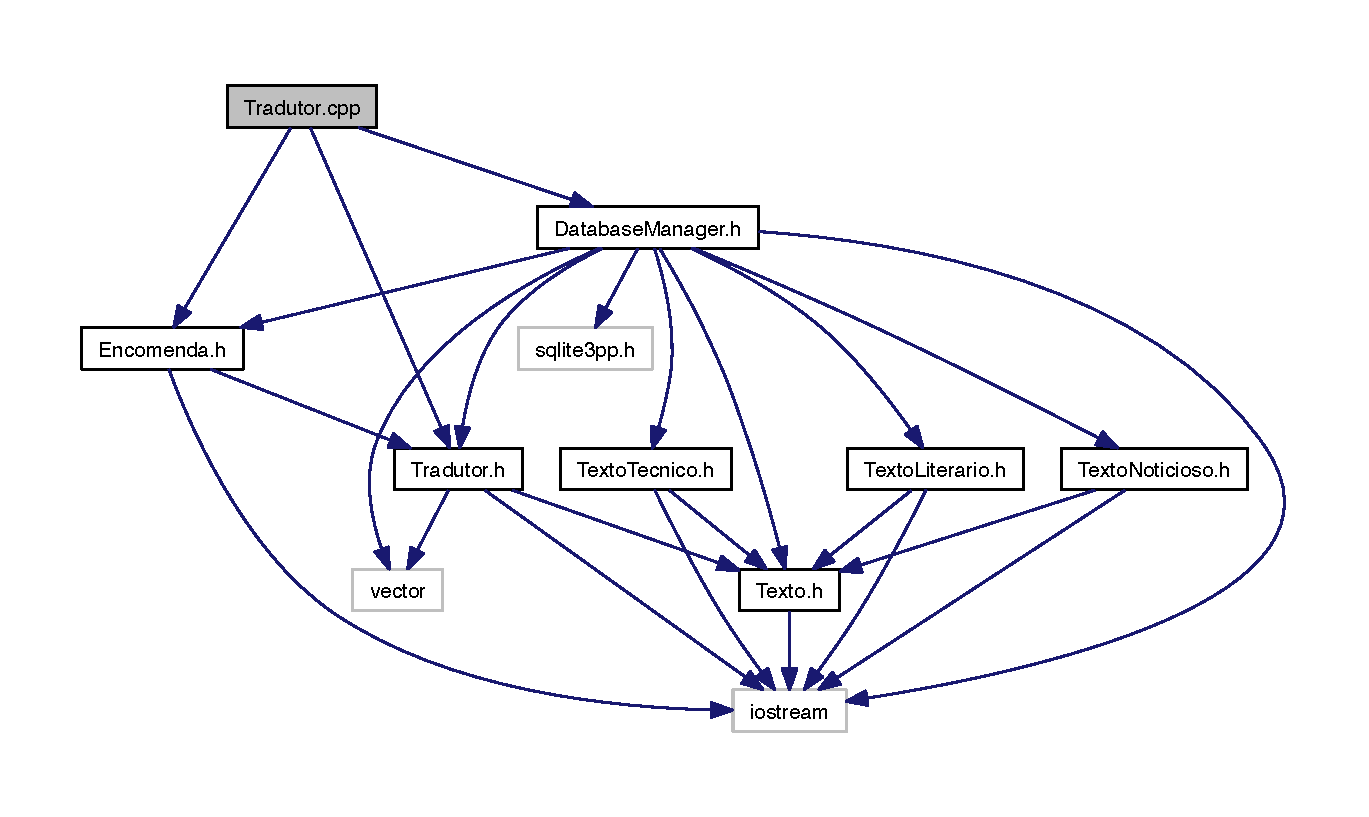
\includegraphics[width=350pt]{_tradutor_8cpp__incl}
\end{center}
\end{figure}
\subsection*{Macros}
\begin{DoxyCompactItemize}
\item 
\#define \hyperlink{_tradutor_8cpp_a0442eefd0d507ff91236f184952f5dfa}{days\-\_\-to\-\_\-seconds}(days)~days $\ast$ 60 $\ast$ 60 $\ast$ 24
\end{DoxyCompactItemize}


\subsection{Macro Definition Documentation}
\hypertarget{_tradutor_8cpp_a0442eefd0d507ff91236f184952f5dfa}{\index{Tradutor.\-cpp@{Tradutor.\-cpp}!days\-\_\-to\-\_\-seconds@{days\-\_\-to\-\_\-seconds}}
\index{days\-\_\-to\-\_\-seconds@{days\-\_\-to\-\_\-seconds}!Tradutor.cpp@{Tradutor.\-cpp}}
\subsubsection[{days\-\_\-to\-\_\-seconds}]{\setlength{\rightskip}{0pt plus 5cm}\#define days\-\_\-to\-\_\-seconds(
\begin{DoxyParamCaption}
\item[{}]{days}
\end{DoxyParamCaption}
)~days $\ast$ 60 $\ast$ 60 $\ast$ 24}}\label{_tradutor_8cpp_a0442eefd0d507ff91236f184952f5dfa}

\hypertarget{_tradutor_8h}{\section{Tradutor.\-h File Reference}
\label{_tradutor_8h}\index{Tradutor.\-h@{Tradutor.\-h}}
}
{\ttfamily \#include $<$iostream$>$}\\*
{\ttfamily \#include $<$vector$>$}\\*
{\ttfamily \#include \char`\"{}Texto.\-h\char`\"{}}\\*
Include dependency graph for Tradutor.\-h\-:
\nopagebreak
\begin{figure}[H]
\begin{center}
\leavevmode
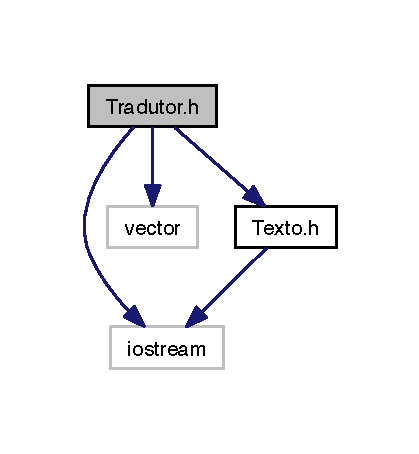
\includegraphics[width=201pt]{_tradutor_8h__incl}
\end{center}
\end{figure}
This graph shows which files directly or indirectly include this file\-:
\nopagebreak
\begin{figure}[H]
\begin{center}
\leavevmode
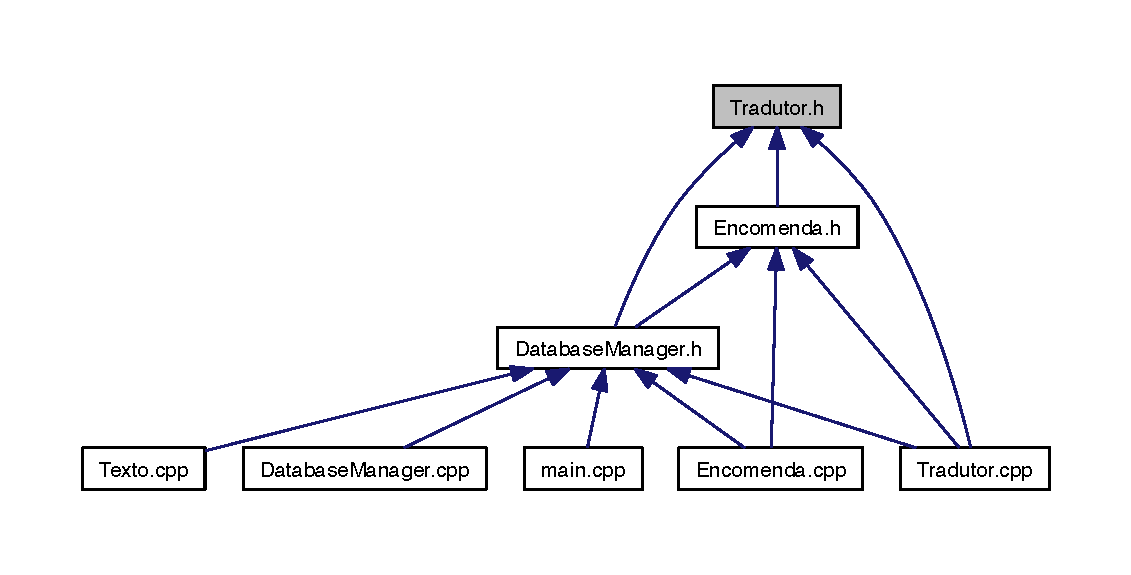
\includegraphics[width=350pt]{_tradutor_8h__dep__incl}
\end{center}
\end{figure}
\subsection*{Classes}
\begin{DoxyCompactItemize}
\item 
class \hyperlink{class_tradutor}{Tradutor}
\begin{DoxyCompactList}\small\item\em \hyperlink{class_tradutor}{Tradutor} class. \end{DoxyCompactList}\end{DoxyCompactItemize}
\subsection*{Enumerations}
\begin{DoxyCompactItemize}
\item 
enum \hyperlink{_tradutor_8h_a5f121f8f8a3004c289fc2f33c3baa5d0}{k\-Operator\-Op} \{ \hyperlink{_tradutor_8h_a5f121f8f8a3004c289fc2f33c3baa5d0ab3b7f80fb2b799d0f3ff1b2c65736293}{k\-Operator\-Op\-Name\-Comparision}
 \}
\end{DoxyCompactItemize}


\subsection{Enumeration Type Documentation}
\hypertarget{_tradutor_8h_a5f121f8f8a3004c289fc2f33c3baa5d0}{\index{Tradutor.\-h@{Tradutor.\-h}!k\-Operator\-Op@{k\-Operator\-Op}}
\index{k\-Operator\-Op@{k\-Operator\-Op}!Tradutor.h@{Tradutor.\-h}}
\subsubsection[{k\-Operator\-Op}]{\setlength{\rightskip}{0pt plus 5cm}enum {\bf k\-Operator\-Op}}}\label{_tradutor_8h_a5f121f8f8a3004c289fc2f33c3baa5d0}
\begin{Desc}
\item[Enumerator]\par
\begin{description}
\index{k\-Operator\-Op\-Name\-Comparision@{k\-Operator\-Op\-Name\-Comparision}!Tradutor.\-h@{Tradutor.\-h}}\index{Tradutor.\-h@{Tradutor.\-h}!k\-Operator\-Op\-Name\-Comparision@{k\-Operator\-Op\-Name\-Comparision}}\item[{\em 
\hypertarget{_tradutor_8h_a5f121f8f8a3004c289fc2f33c3baa5d0ab3b7f80fb2b799d0f3ff1b2c65736293}{k\-Operator\-Op\-Name\-Comparision}\label{_tradutor_8h_a5f121f8f8a3004c289fc2f33c3baa5d0ab3b7f80fb2b799d0f3ff1b2c65736293}
}]\end{description}
\end{Desc}

%--- End generated contents ---

% Index
\newpage
\phantomsection
\addcontentsline{toc}{part}{Index}
\printindex

\end{document}
